% !TEX encoding = UTF-8 Unicode
\documentclass[fleqn,twoside]{article}
\usepackage[ngerman]{babel}
\usepackage[utf8]{inputenc}
\usepackage[T1]{fontenc}
\usepackage{amsmath}
\usepackage{amssymb}
\usepackage{booktabs}
\usepackage{calligra}
\usepackage{cite}
\usepackage{comment}
\usepackage{csquotes}
\usepackage{enumitem}
\usepackage{eurosym}
\usepackage{fancyhdr}
\usepackage{fdsymbol}
\usepackage{float}
\usepackage{graphicx}
\usepackage{graphicx}
\usepackage{multirow}
\usepackage{nicefrac}
\usepackage{pdfpages}
\usepackage{pifont}
\usepackage{romanbar}
\usepackage{siunitx}
\usepackage{stanli}
\usepackage{svg}
\usepackage{tabto}
\usepackage{tabularx}
\usepackage{textcomp}
\usepackage{tikz}
\usepackage{titlesec}
\usepackage{todonotes}
\usepackage{wasysym}
\usepackage{wrapfig}
\usepackage{yfonts}
%\usepackage{3dstructuralanalysis}
%\usepackage{emerald}
%\usepackage{structuralanalysis}
%\usepackage{units}



%Befehle abändern
%Itemize ohne Lücken
\setlist[itemize]{noitemsep, topsep=2pt}
\raggedbottom
%\renewcommand{\todo}[1]{\todo[inline]{#1}}


%Betragsfunktion
\newcommand{\abs}[1]{\ensuremath{\left\vert#1\right\vert}}
%Einheitenfunktion
\newcommand{\un}[2]{{\unit[#1]{\color{black!100}[#2]}}}

\usepackage[pdftex, colorlinks, linkcolor=black, frenchlinks]{hyperref}
\usepackage[a4paper , lmargin = {2.5cm} , rmargin = {2cm} , tmargin = {2.5cm} , bmargin = {2.5cm} ]{geometry}
\pagestyle{fancy}

\title{\Huge{\textfrak{Bauwerkserhaltung im Holzbau}}}
\author{\calligra{Jonas Konrad}}
\date{\textfrak{\today}}

\begin{document}
\parindent 0pt
\fancyhead[L]{Jonas Konrad}
\fancyfoot[L]{\frakfamily J. K.}
\fancyfoot[R]{\frakfamily }
\fancyfoot[C]{\frakfamily "Das lassen wir jetzt einfach mal so stehen" \\Seite \thepage}
\maketitle \thispagestyle{empty}
%\initfamily %Für Initialien
\begin{center}
\textfrak{Diese Sammlung der Vorlesungsinhalte wurde im Wintersemester 2022/23 von Jonas Konrad verfasst.\\Dozent: PD Dr.-Ing. Matthias Frese , Übungsleiter: M.Sc. Sebastian Egner\\Kein Anspruch auf Vollständigkeit oder Fehlerfreiheit.\\LaTex Vorlage: github.com/Neowise33}
\end{center}
\tableofcontents
%\listoftodos
\newpage

%\listoftodos
%\newpage



\section{Klausurfragen:}
    \begin{itemize}
        \item Berechnung Stirnversatz inkl. Verstärkung mit VGS \\
        Vorholz schert ab - wie reparieren?\\
        Wie verstärken, falls noch nicht ganz versagt?\\
        Schubspannung im Vorholz zeichnen\\
        Warum $l_v$ nicht unendlich lang machen?
        \item Kraftflüsse Bauwerk/Dächer bestimmen
        \item Aufbau von Dächern benennen
        \item Baudenkmalkonzepte nennen und markante Eigenschaften
        \item Bohrwiderstandsmessung interpretieren
        \item Weiches oder hartes Holz für Anwendungen verwenden? Vor- und Nachteile
        \item Holzschädlinge, Pilze, Insekten\\
        Wo treten sie auf?\\ 
        Bedingungen?\\
        Welcher ist der kritischste?
        \item Pfosten, Geschoss, Stockwerksbau\\
        Bezeichnen, Unterschiede, Vorteile nennen
        \item Historisches Tragwerk\\
        Vorgehen Sanierung, Nachweise und Schnittkräfte
        \item Definition $k_{cr}$ (Beiwert Schubbeanspruchbarkeit) \\
        Prüfung für $k_{cr}=1$?(keine Schwindrisse in Scherebene, siehe Stirnversätze)
        \item Biegenachweis Bauteil Bestand nicht eingehalten?\\
        Visuelle Begutachtung um Sortierklassen zu erhöhen
    \end{itemize}



\newpage
\section{Geschichte des Holzbaus}


\subsection{Kettenbindung}
Auch \enquote{heute} noch begegnen uns archaische Formen der Holzverbindungen. Ein Beispiel hierfür ist die
in der DIN 4420:1955 dargestellte Kettenbindung mit dem T-Eisenschloss (siehe nachstehende
Illustration im Bild 4). Es war demnach üblich, Rundhölzer zum Zwecke des Gerüstbaus mit Ketten zu
verbinden.
\begin{center} 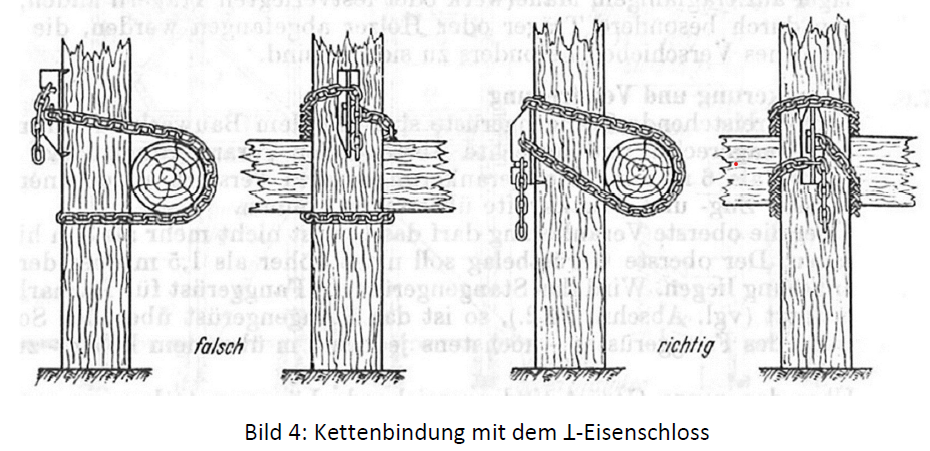
\includegraphics[width=0.55\textwidth]{Grafiken/Geschichte des Holzbaus/Kettenbindungen.png} \end{center}

\subsection{Geschoss- bzw. Ständerbau}
    \begin{minipage}{0.6\textwidth}
    \begin{itemize}
        \item Geschoss, vgl. schießen in der alten Bedeutung von aufschießen oder in die Höhe ragen
        \item Weiterentwicklung des Pfostenbaus
        \item Keine Einspannung von Pfosten im Erdreich/Baugrund\\
        $\rightarrow$ Verbesserung der Dauerhaftigkeit\\
        $\rightarrow$ Aussteifungselemente erforderlich
        \item Ständer durchlaufend von (Stein)Sockel bzw. Schwellenkranz in der Regel bis zur Traufe und zum
        First
        \item Streben (oder Schwertungen) der Aussteifung verlaufen u. U. über mehrere Etagen
        \item Geschossbalken einzelner Etagen sind gezapft, geblattet oder durchgezapft, z. B Ankerbalken mit
        Zapfenschlössern
        \item Geschossbau tritt in Verbindung mit dem Stockwerksbau auf
        \item Mit einer zunehmenden Besiedelungsdichte in den Städten und den damit beengten räumlichen
        Verhältnissen später durch den Stockwerksbau abgelöst (Das Abbinden großflächiger Bundachsen
        braucht Platz!)
    \end{itemize}
    \end{minipage}
    \begin{minipage}{0.4\textwidth}
        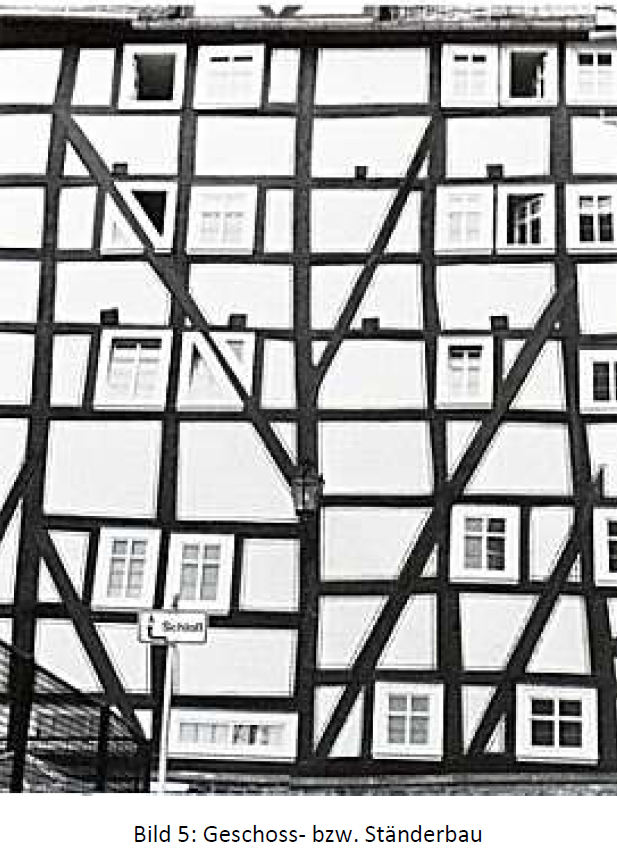
\includegraphics[width=0.9\textwidth]{Grafiken/Geschichte des Holzbaus/Geschoss- bzw. Staenderbau.png}
    \end{minipage}
    
    
\subsection{Stockwerksbau}
    \begin{minipage}{0.6\textwidth}
    \begin{itemize}
        \item Löst den Geschoss- bzw. Ständerbau ab
        \item Einzelne Nutzebenen bilden in sich abgeschlossene Konstruktionseinheiten (modulare Bauweise)
        \item Statt langer Streben, werden i. d. R. Fuß- und Kopfbänder als Aussteifung eingebaut
        \item Auskragungen möglich, weil Deckenbalken über die Grundfläche der darunterliegenden Etagen geführt werden können $\rightarrow$ Vergrößerung der Etagenfläche
        \item Grat- bzw. Stichbalken ermöglichen umlaufende Auskragungen, die über Knaggen unterseitig gestützt werden
        \item Fachwerkhäuser in Stockwerksbauweise wirken in der Regel strukturierter (Ständer werden über den Deckenbalken angeordnet) im Vergleich zu solchen in Geschossbauweise
    \end{itemize}
    \end{minipage}
    \begin{minipage}{0.4\textwidth}
        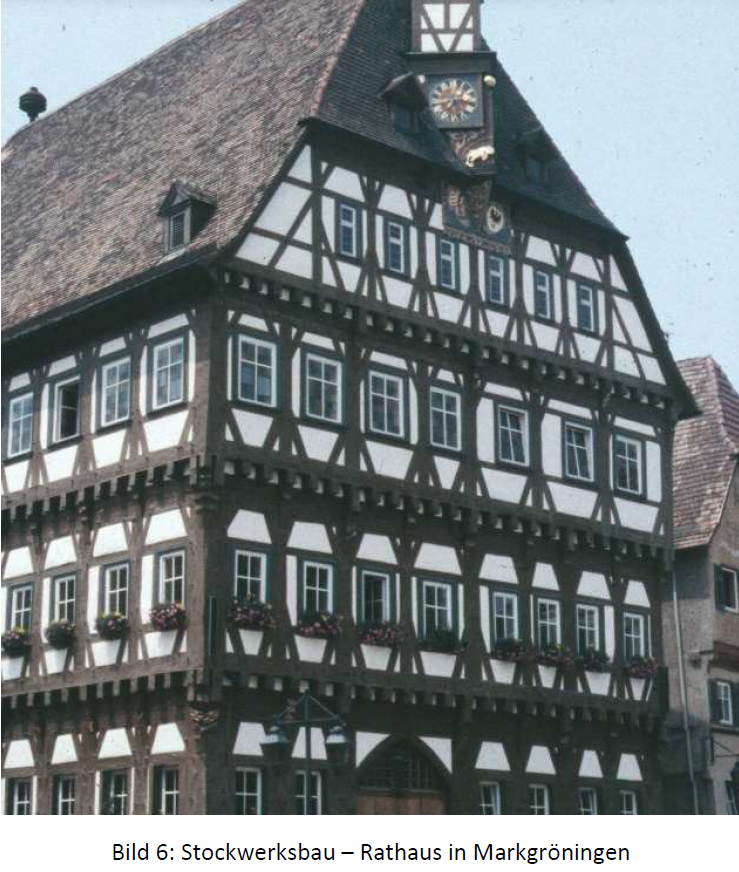
\includegraphics[width=0.9\textwidth]{Grafiken/Geschichte des Holzbaus/Stockwerksbau.png}
    \end{minipage}
    
\subsection{Übersicht Begriffe Fachwerksbau}
\begin{center}
\scriptsize
    \includesvg[width=0.6\textwidth]{Grafiken/Geschichte des Holzbaus/Timber_framing_elements.svg}
\scriptsize
\end{center}
    

\newpage
\section{Dachbauweisen}
    
    \subsection{Grundbegriffe:}
        \begin{itemize}
            \item Sprengwerk: Eine meist hölzerne Konstruktion zur Aufnahme großer Lasten bzw. zur Überbrückung großer Spannweiten
            \item Spannriegel: waagrechter von Streben verspannter Balken (eines Sprengwerks)
        \end{itemize}
    
    \subsection{Übersicht Dachbauweisen:}
        \begin{minipage}{0.45\textwidth}
            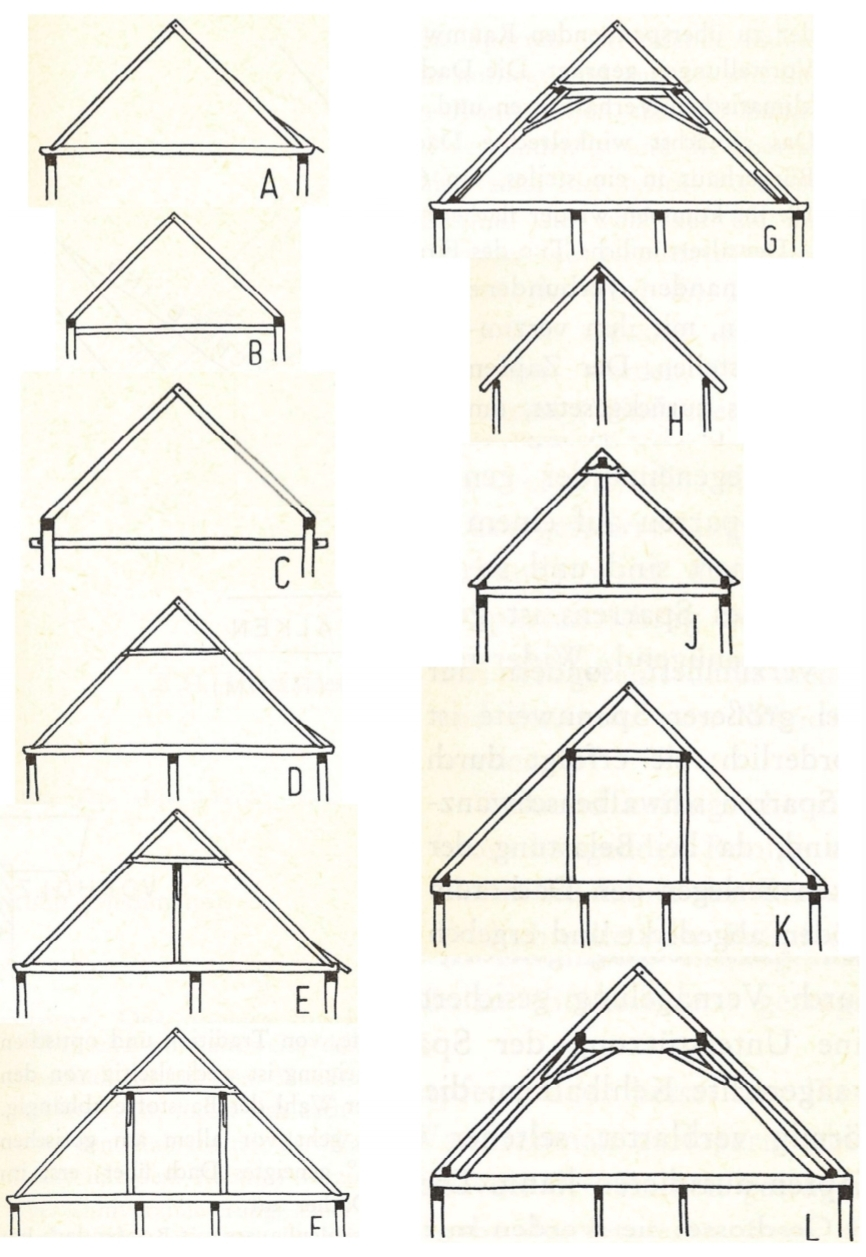
\includegraphics[width=1\textwidth]{Grafiken/Daecher/Uebersicht Daecher.jpg}
        \end{minipage}
        \begin{minipage}{0.55\textwidth}
            \begin{enumerate}[label=(\Alph*)]
                \item Sparrendach mit optionalem Aufschiebling
                \item Sparrendach mit Oberrähmverzimmerung
                \item Sparrendach mit Ankerbalken und Zapfenschloss
                \item Kehlbalkendach mit links angeblattetem und rechts eingezapftem Kehlbalken und optionalem Aufschiebling
                \item Kehlbalkendach mit einfachem stehendem Stuhl und optionalem Aufschiebling
                \item Kehlbalkendach mit doppeltem stehendem Stuhl und längsversteif durch obere Bügen
                \item Kehlbalkendach mit doppeltem liegendem Stuhl, der durch obere und untere Bügen längsversteift ist
                \item Pfettendach mit Firstsäule
                \item -
                \item Pfettendach mit abgefangener Firstsäule oder mit einfachem stehendem Stuhl und Zange
                \item Pfettendach mit doppeltem stehendem Stuhl
                \item Pfettendach mit doppeltem liegendem Stuhl und oberen Bügen
            \end{enumerate}
        \end{minipage}
            
    \subsection{Historischer Fußpunkt Dach:}
            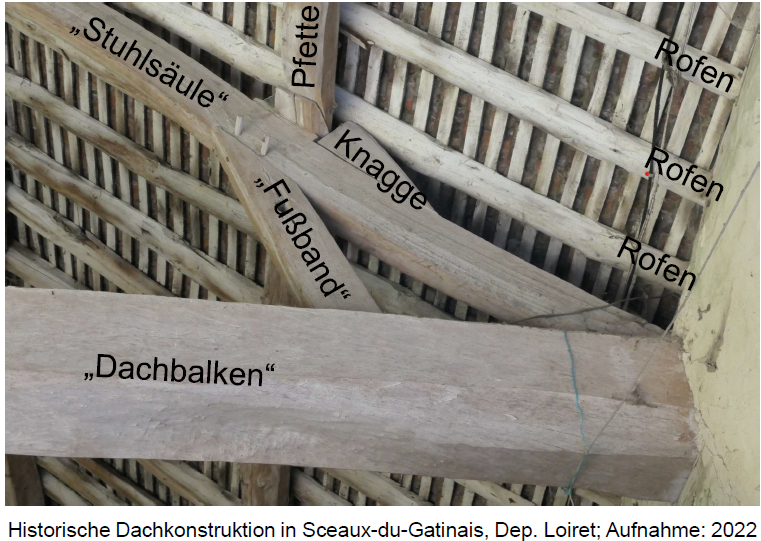
\includegraphics[width=0.45\textwidth]{Grafiken/Daecher/Historischer_Fusspunkt_Dach.png}
    \subsection{Kehlbalkendach:}
            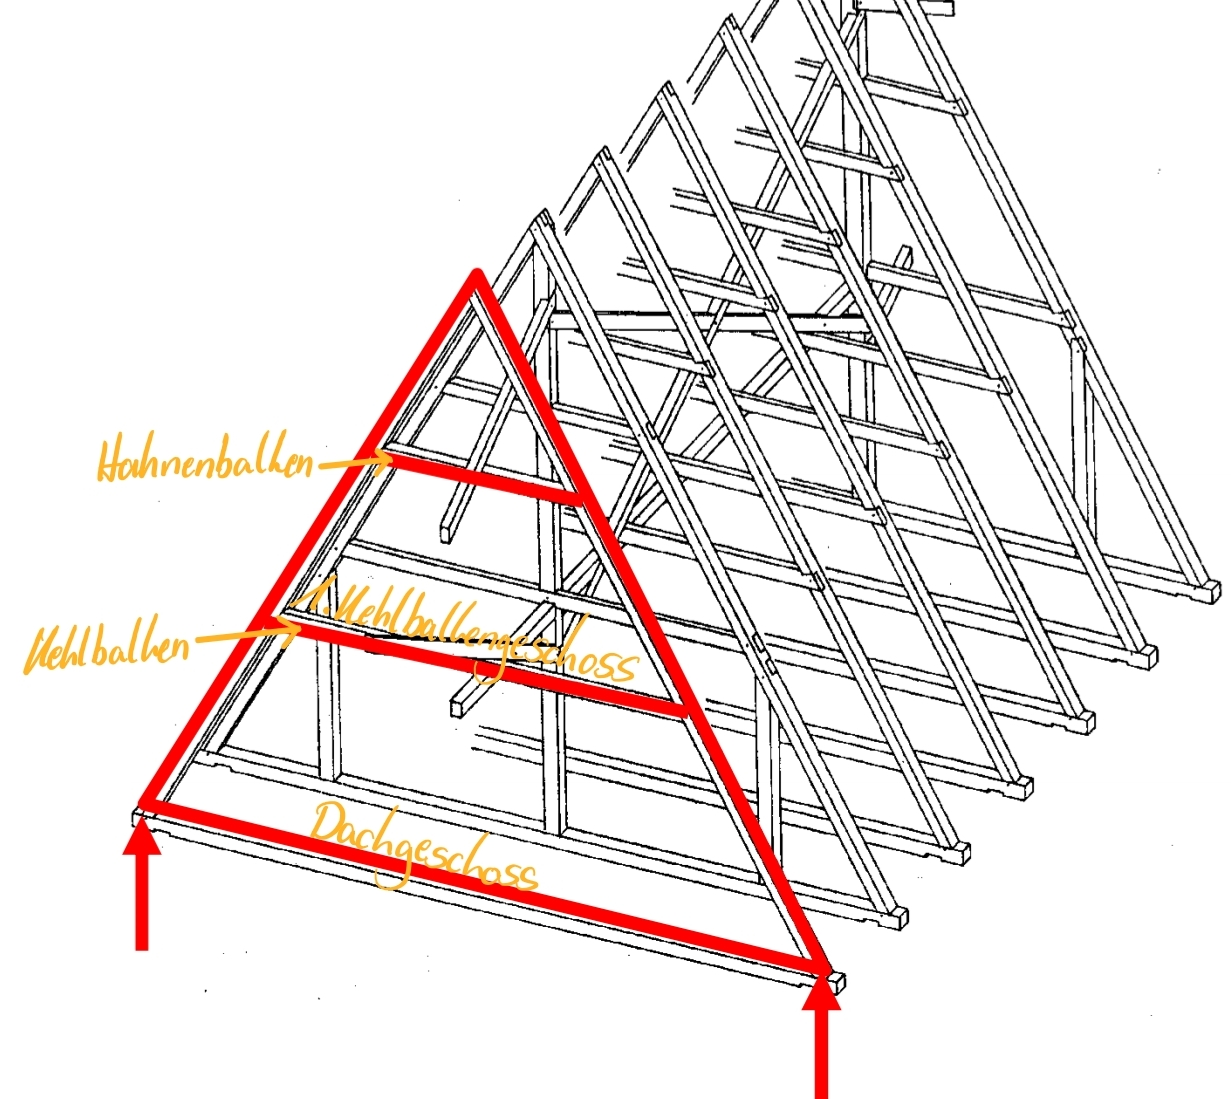
\includegraphics[width=0.45\textwidth]{Grafiken/Daecher/Sparrendach mit Kehlbalken.jpg}
            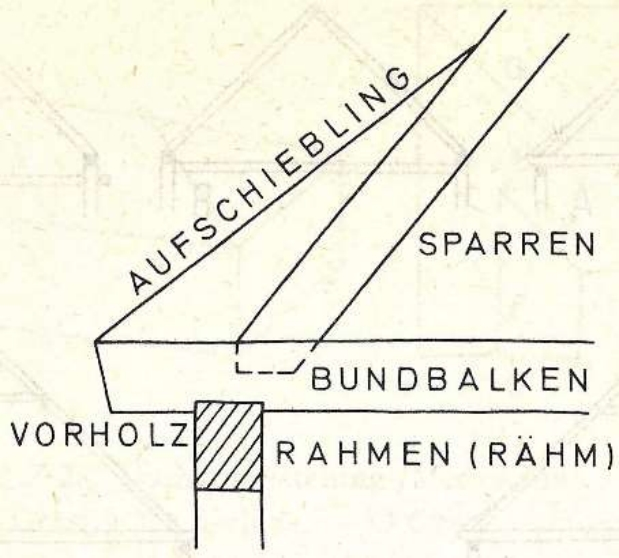
\includegraphics[width=0.45\textwidth]{Grafiken/Daecher/Sparrendach Fusspunktausbildung.jpg}\\
            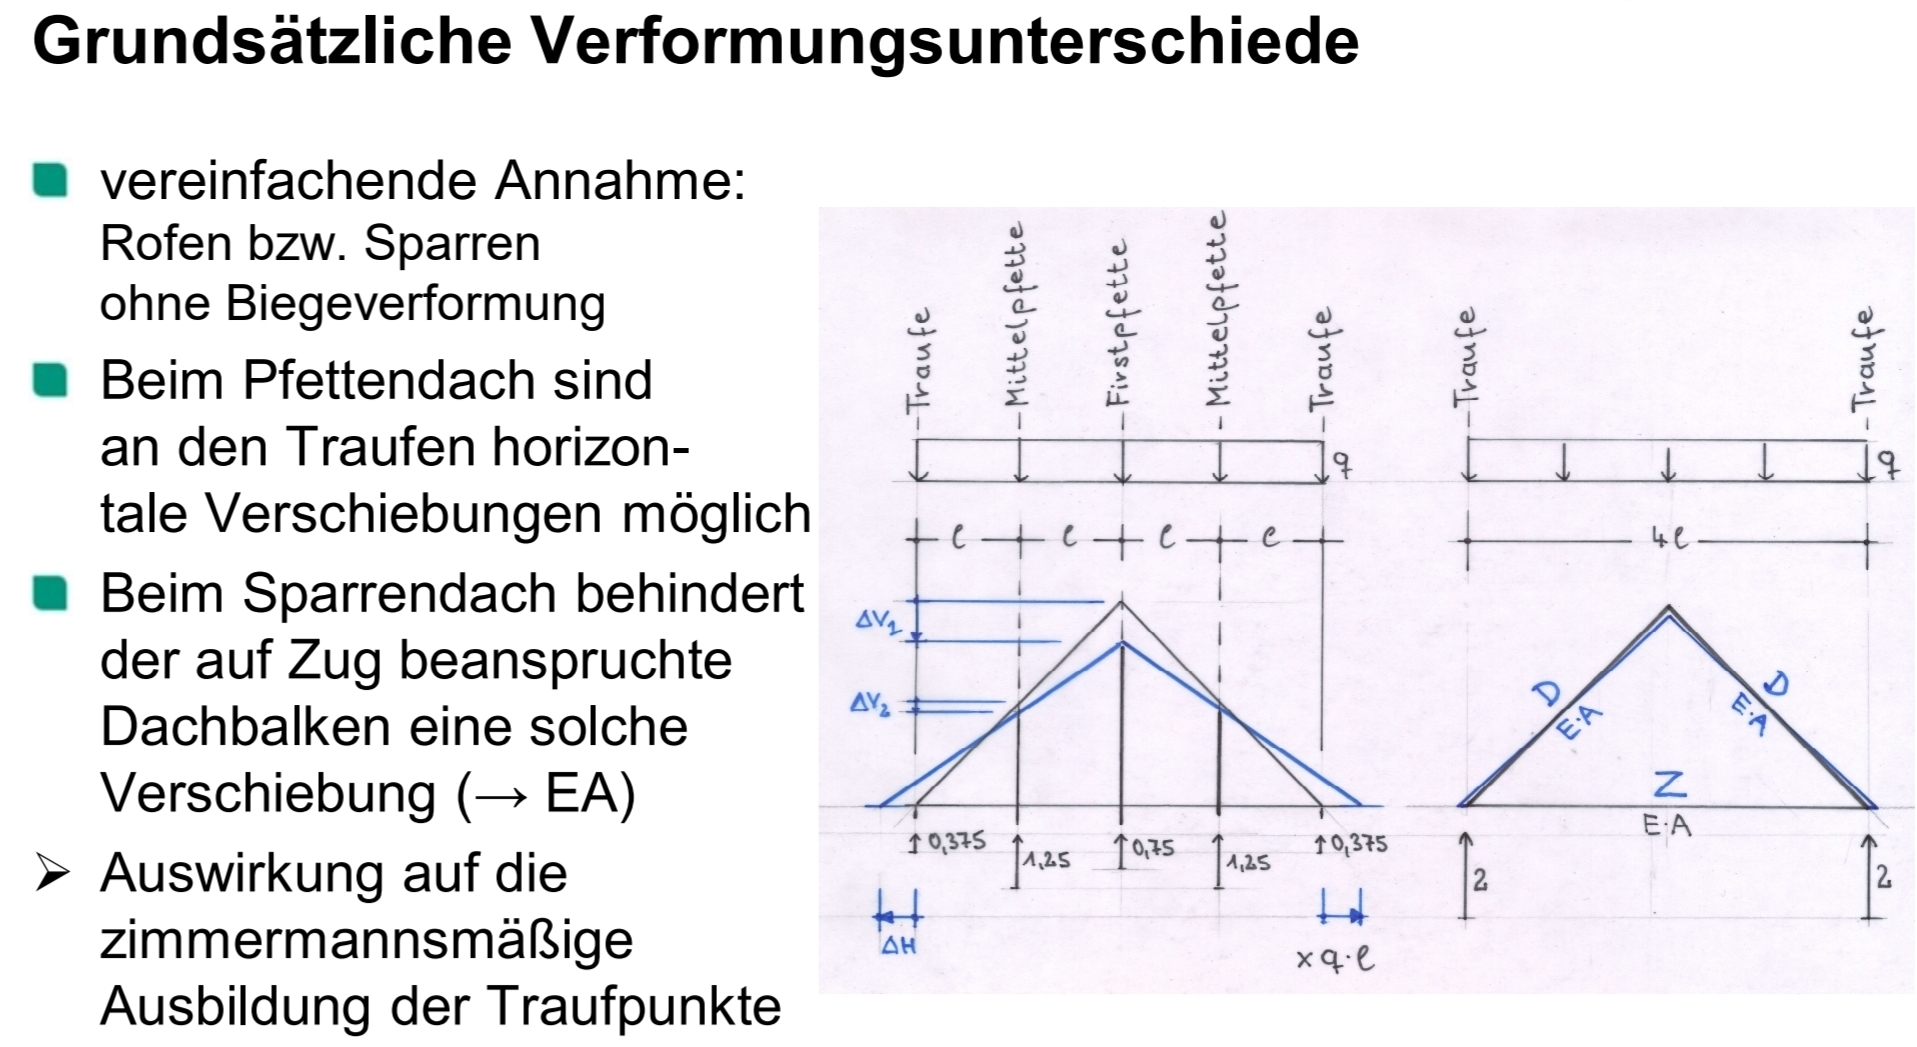
\includegraphics[width=0.45\textwidth]{Grafiken/Daecher/Sparrendach Verformung.jpg}
    \subsection{Stuhlrähm:}
            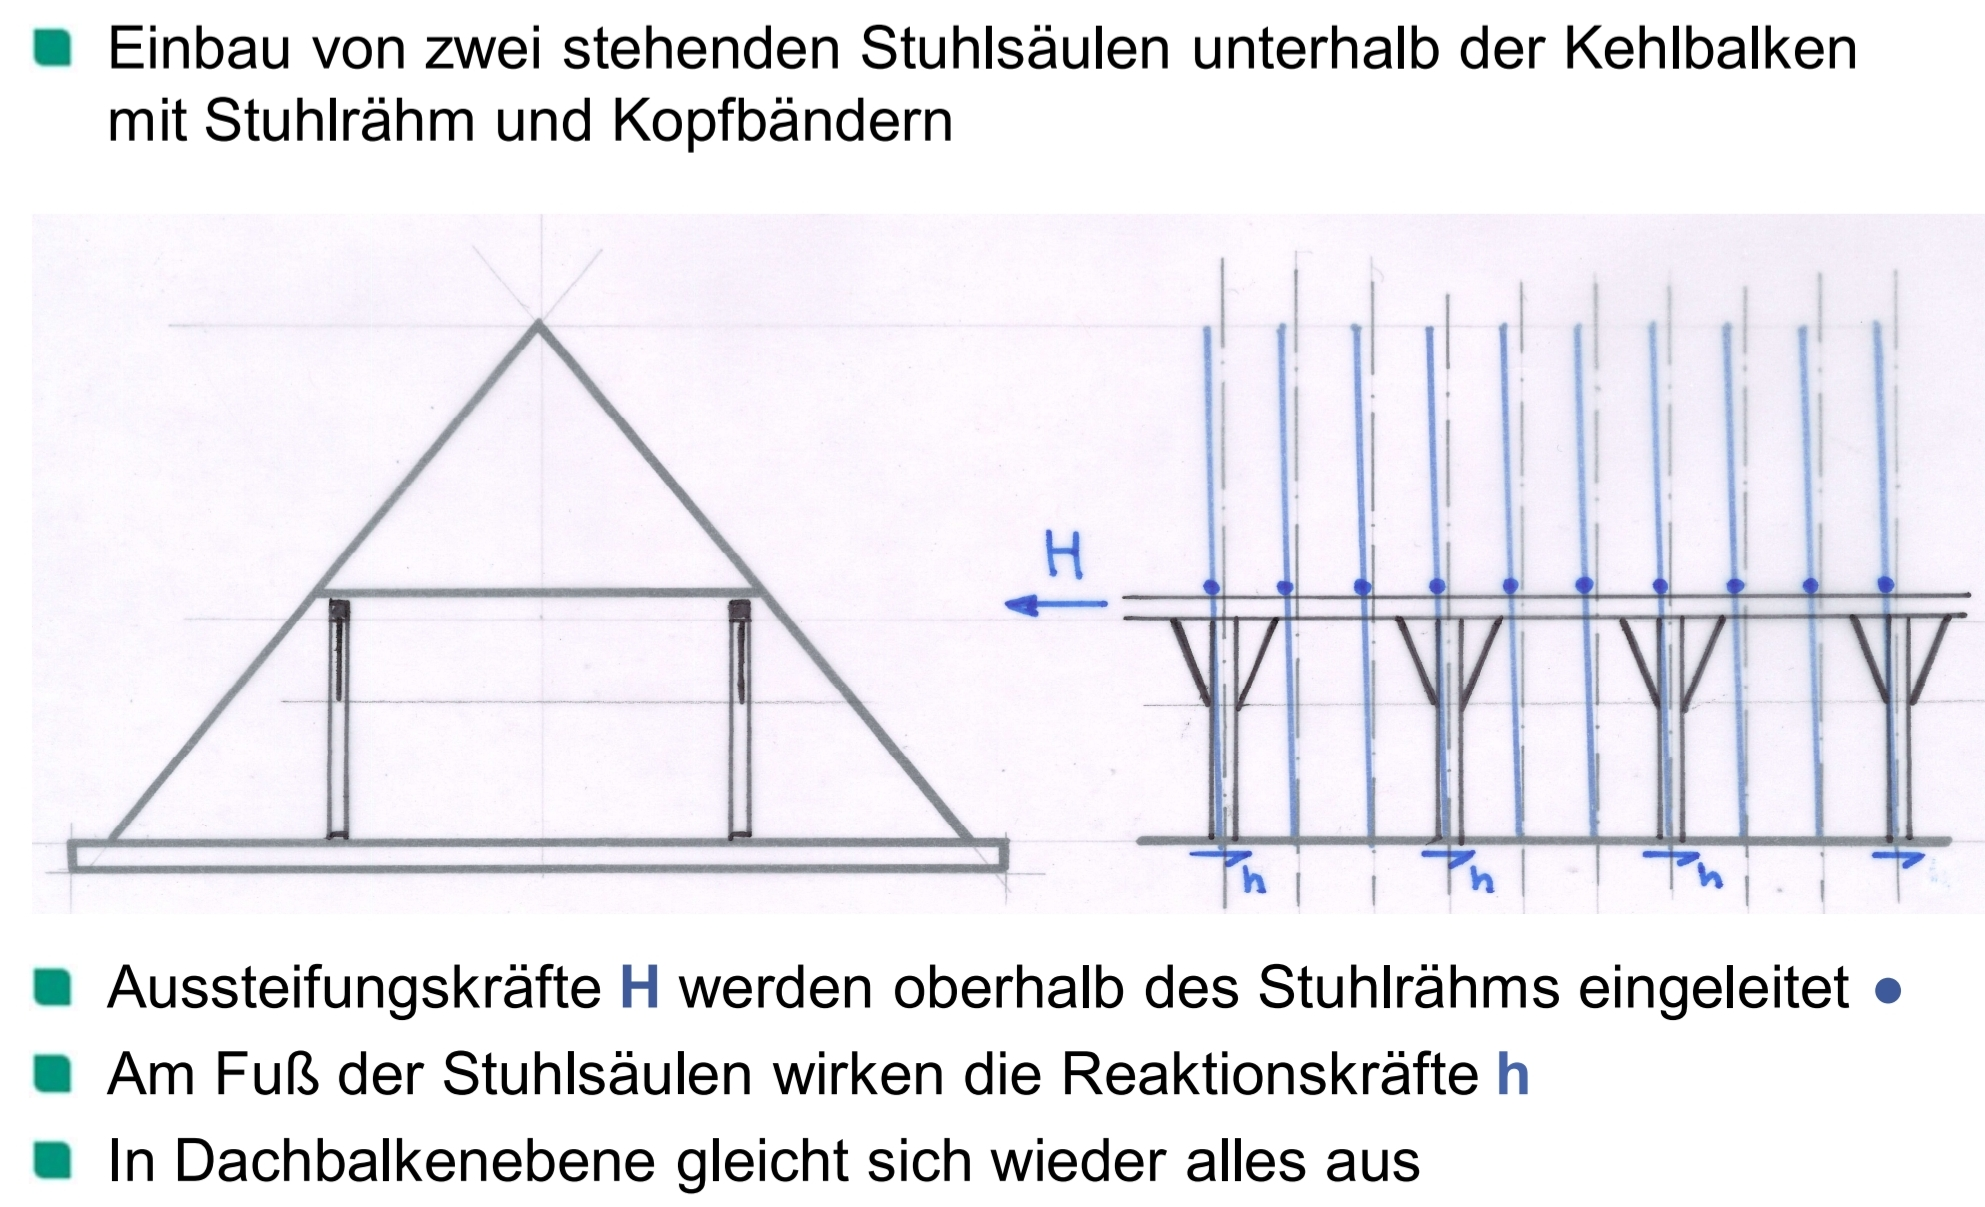
\includegraphics[width=0.45\textwidth]{Grafiken/Daecher/Kehlbalkendach mit Stuhlraehm und Kopfbaendern.jpg}
            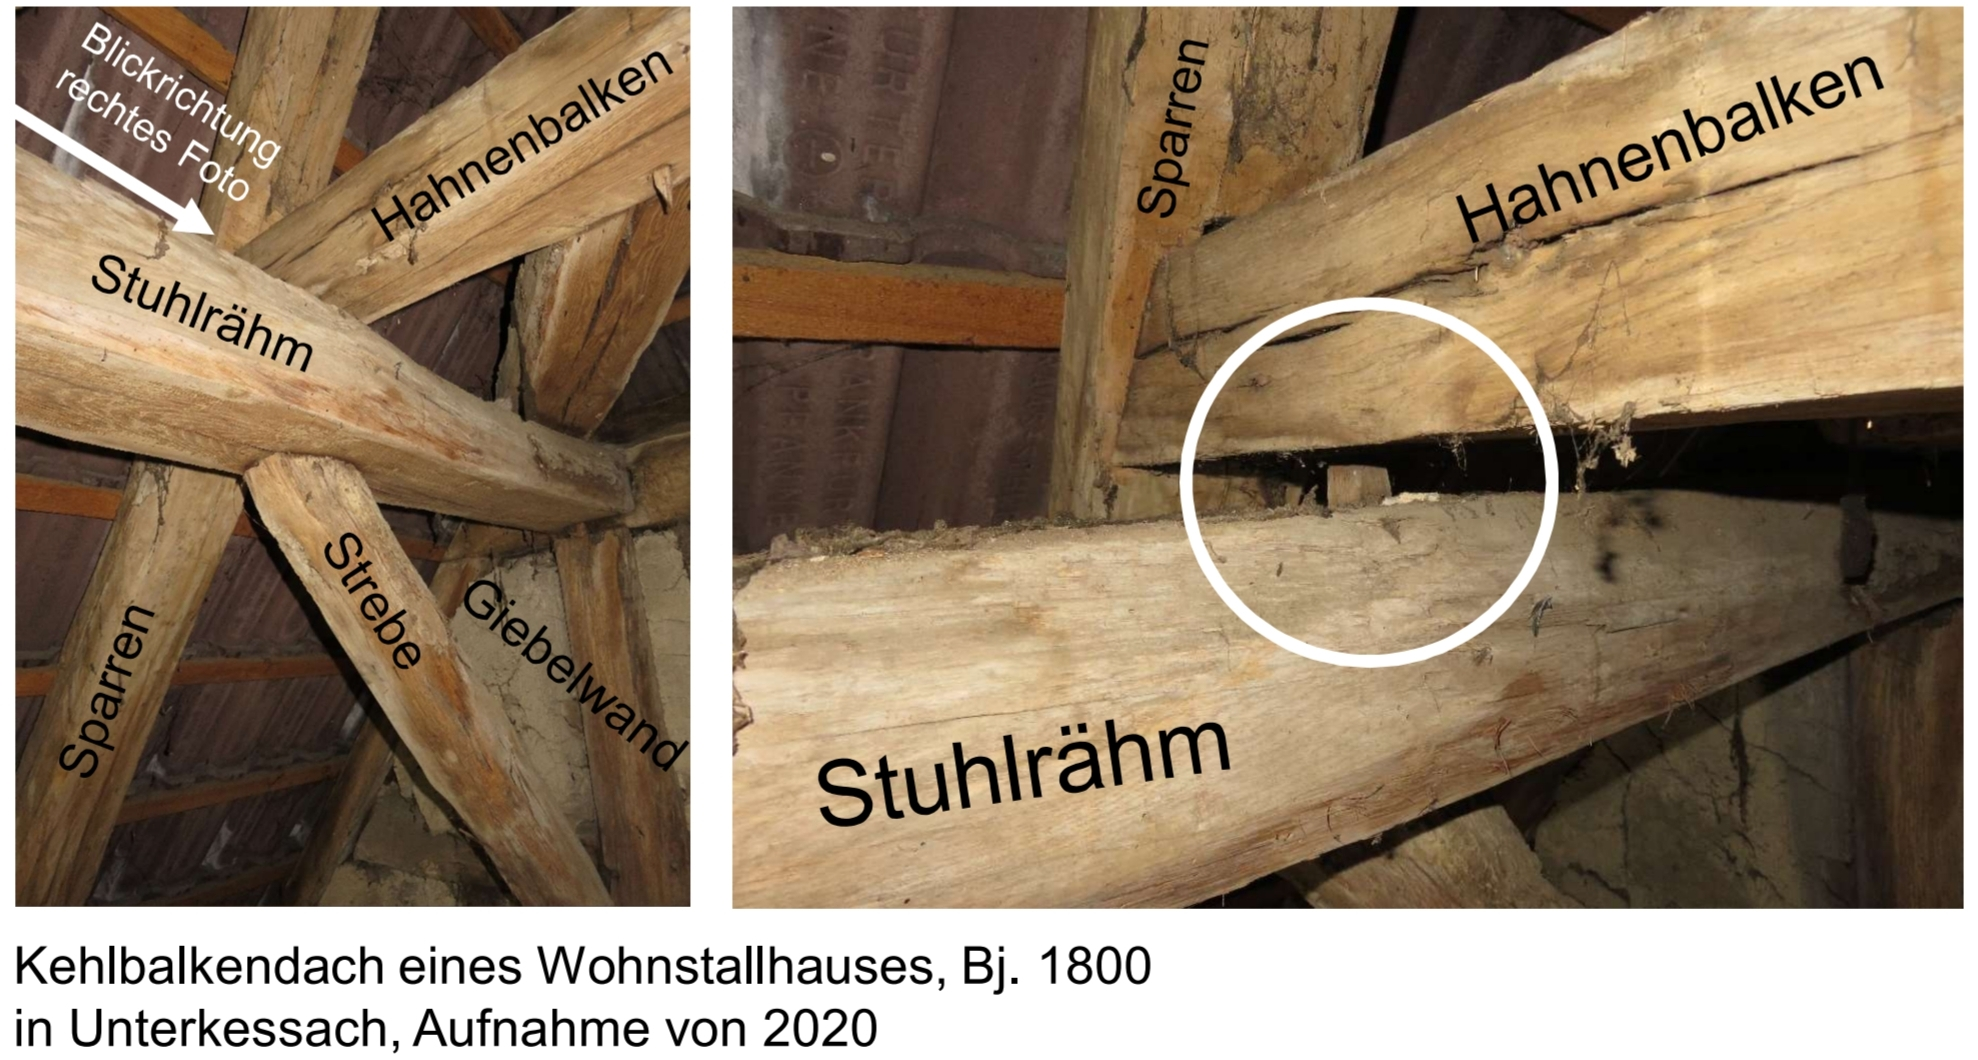
\includegraphics[width=0.45\textwidth]{Grafiken/Daecher/Verbindung Stuhlraehm Hahnenbalken.jpg}\\
            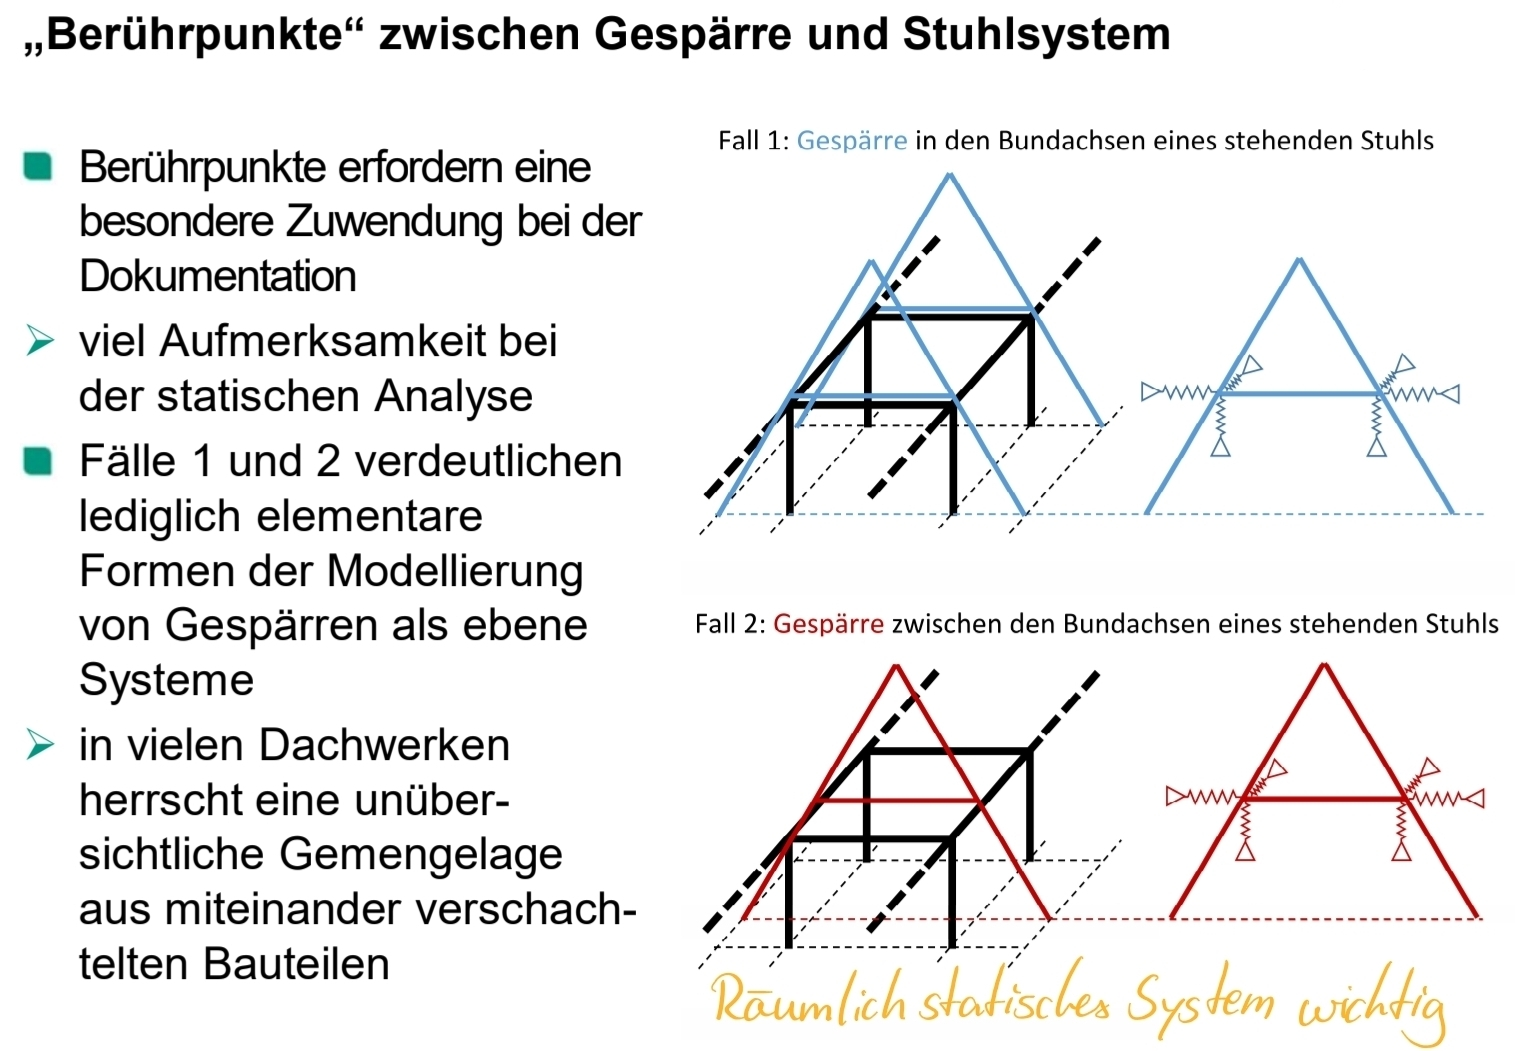
\includegraphics[width=0.45\textwidth]{Grafiken/Daecher/Gespaerre und Stuhlsystem Beruehrpunkt.png}
            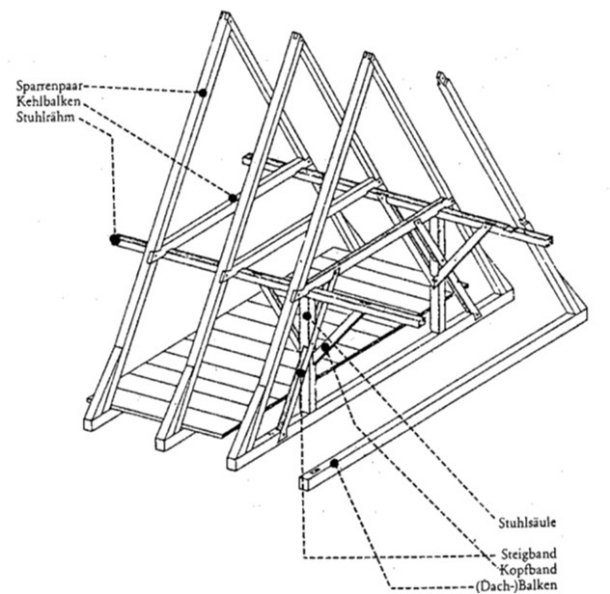
\includegraphics[width=0.45\textwidth]{Grafiken/Daecher/Kehlbalkendach mit Stuhlraehm.jpg}\\
            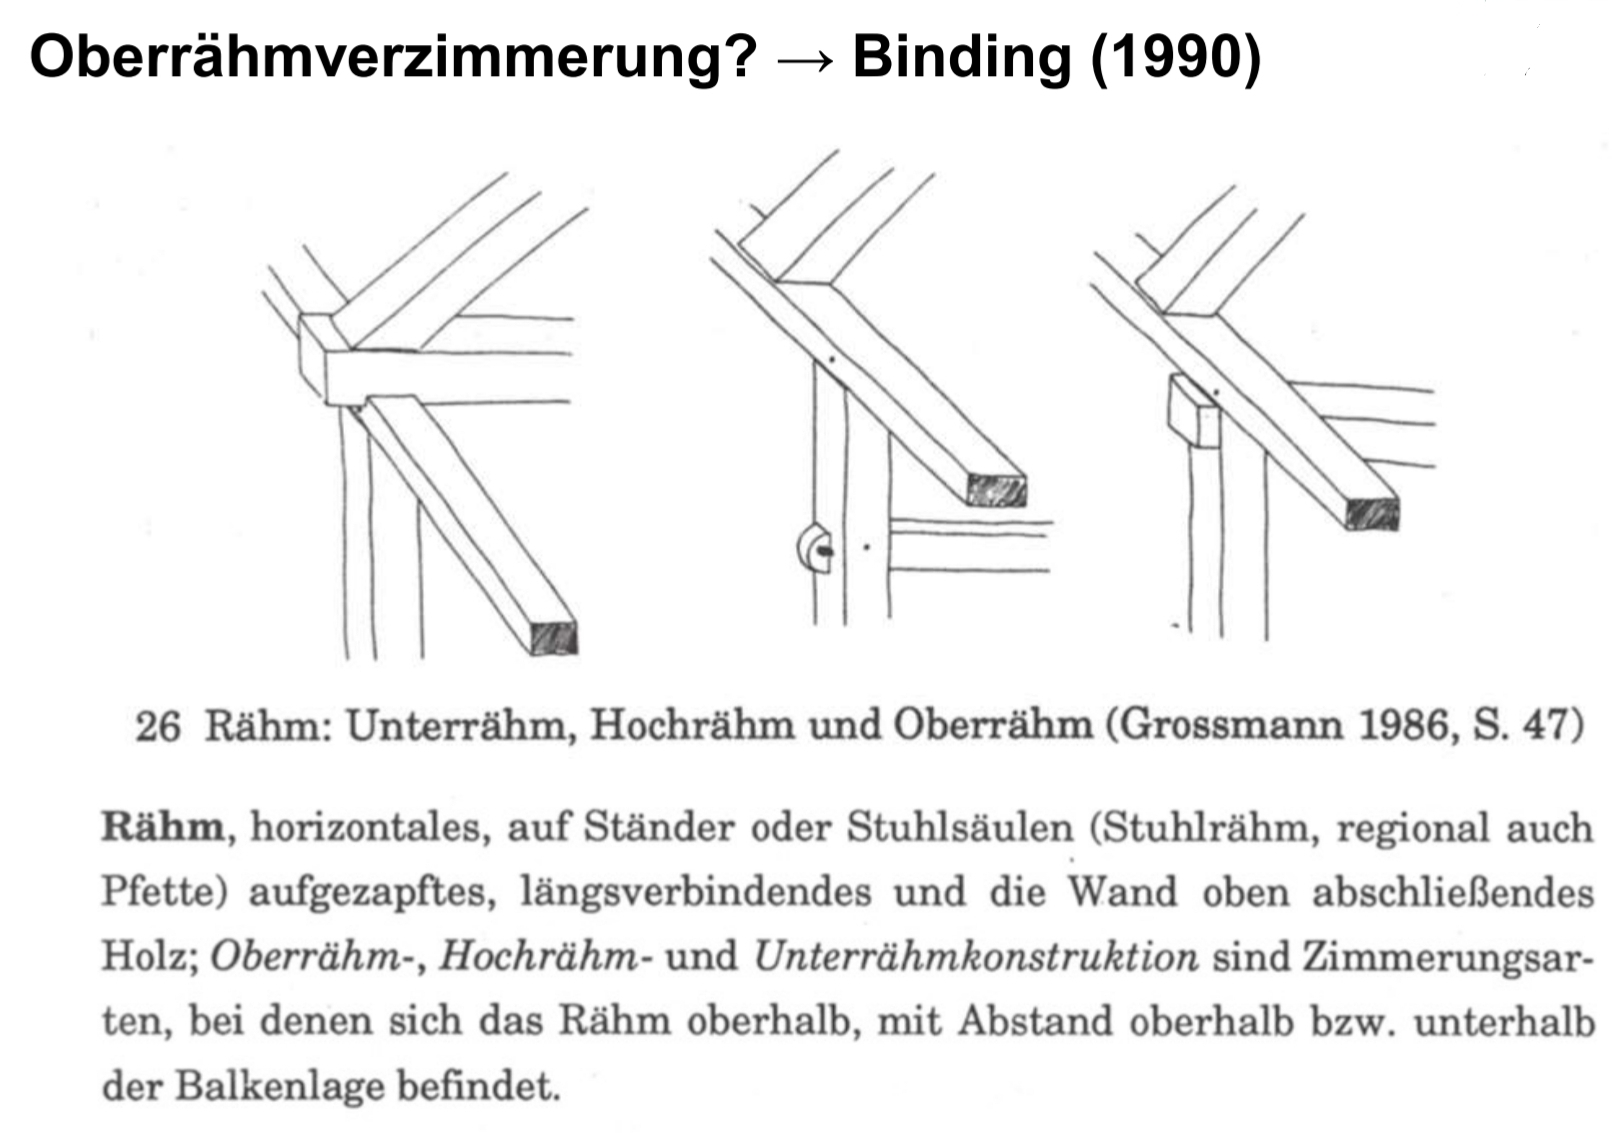
\includegraphics[width=0.45\textwidth]{Grafiken/Daecher/Oberraehmverzimmerung.jpg}
    \subsection{Pfettendach:}
            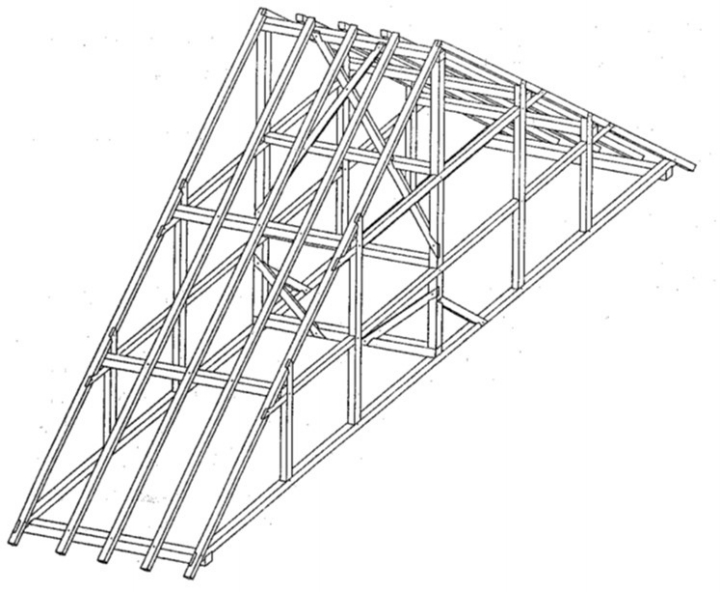
\includegraphics[width=0.35\textwidth]{Grafiken/Daecher/Pfettendach.png}
    \subsection{Liegender Stuhl:}
            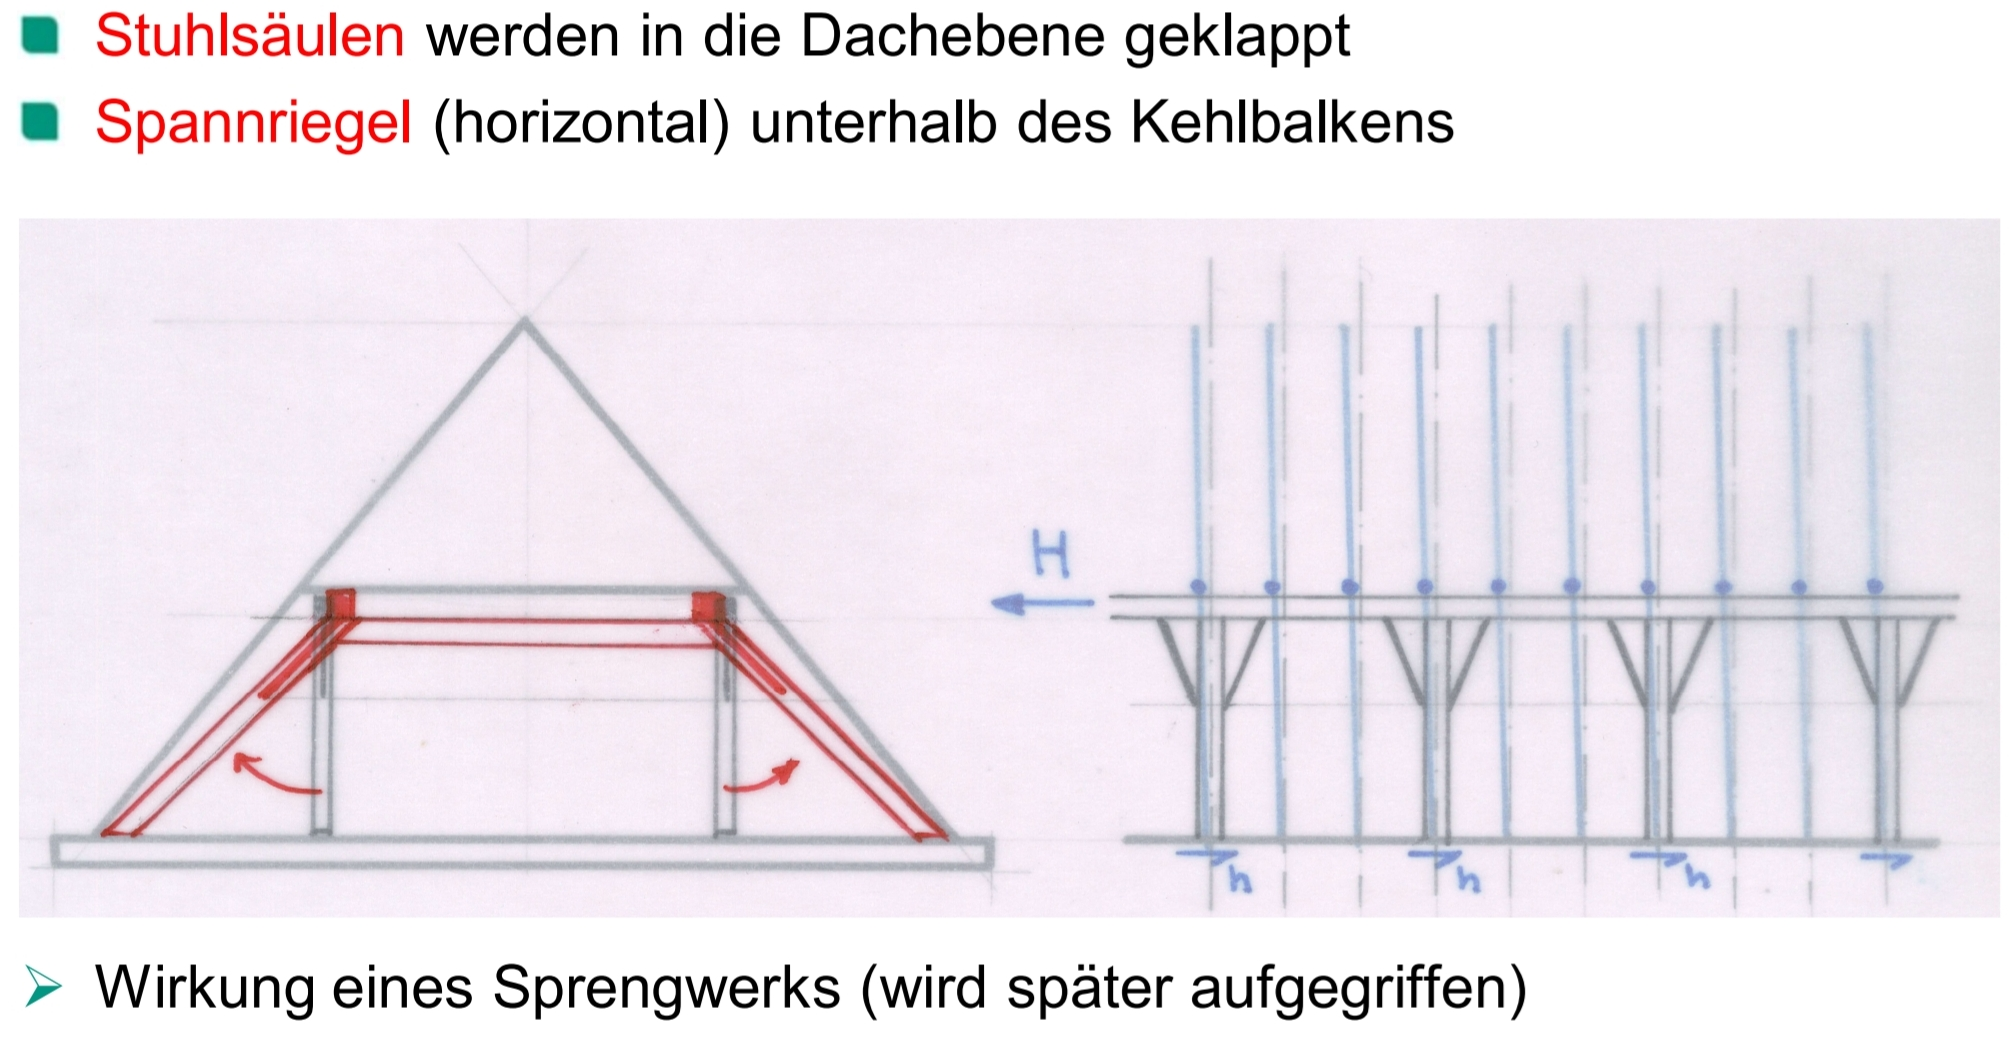
\includegraphics[width=0.45\textwidth]{Grafiken/Daecher/Funktionsweise Sprengwerk.jpg}
            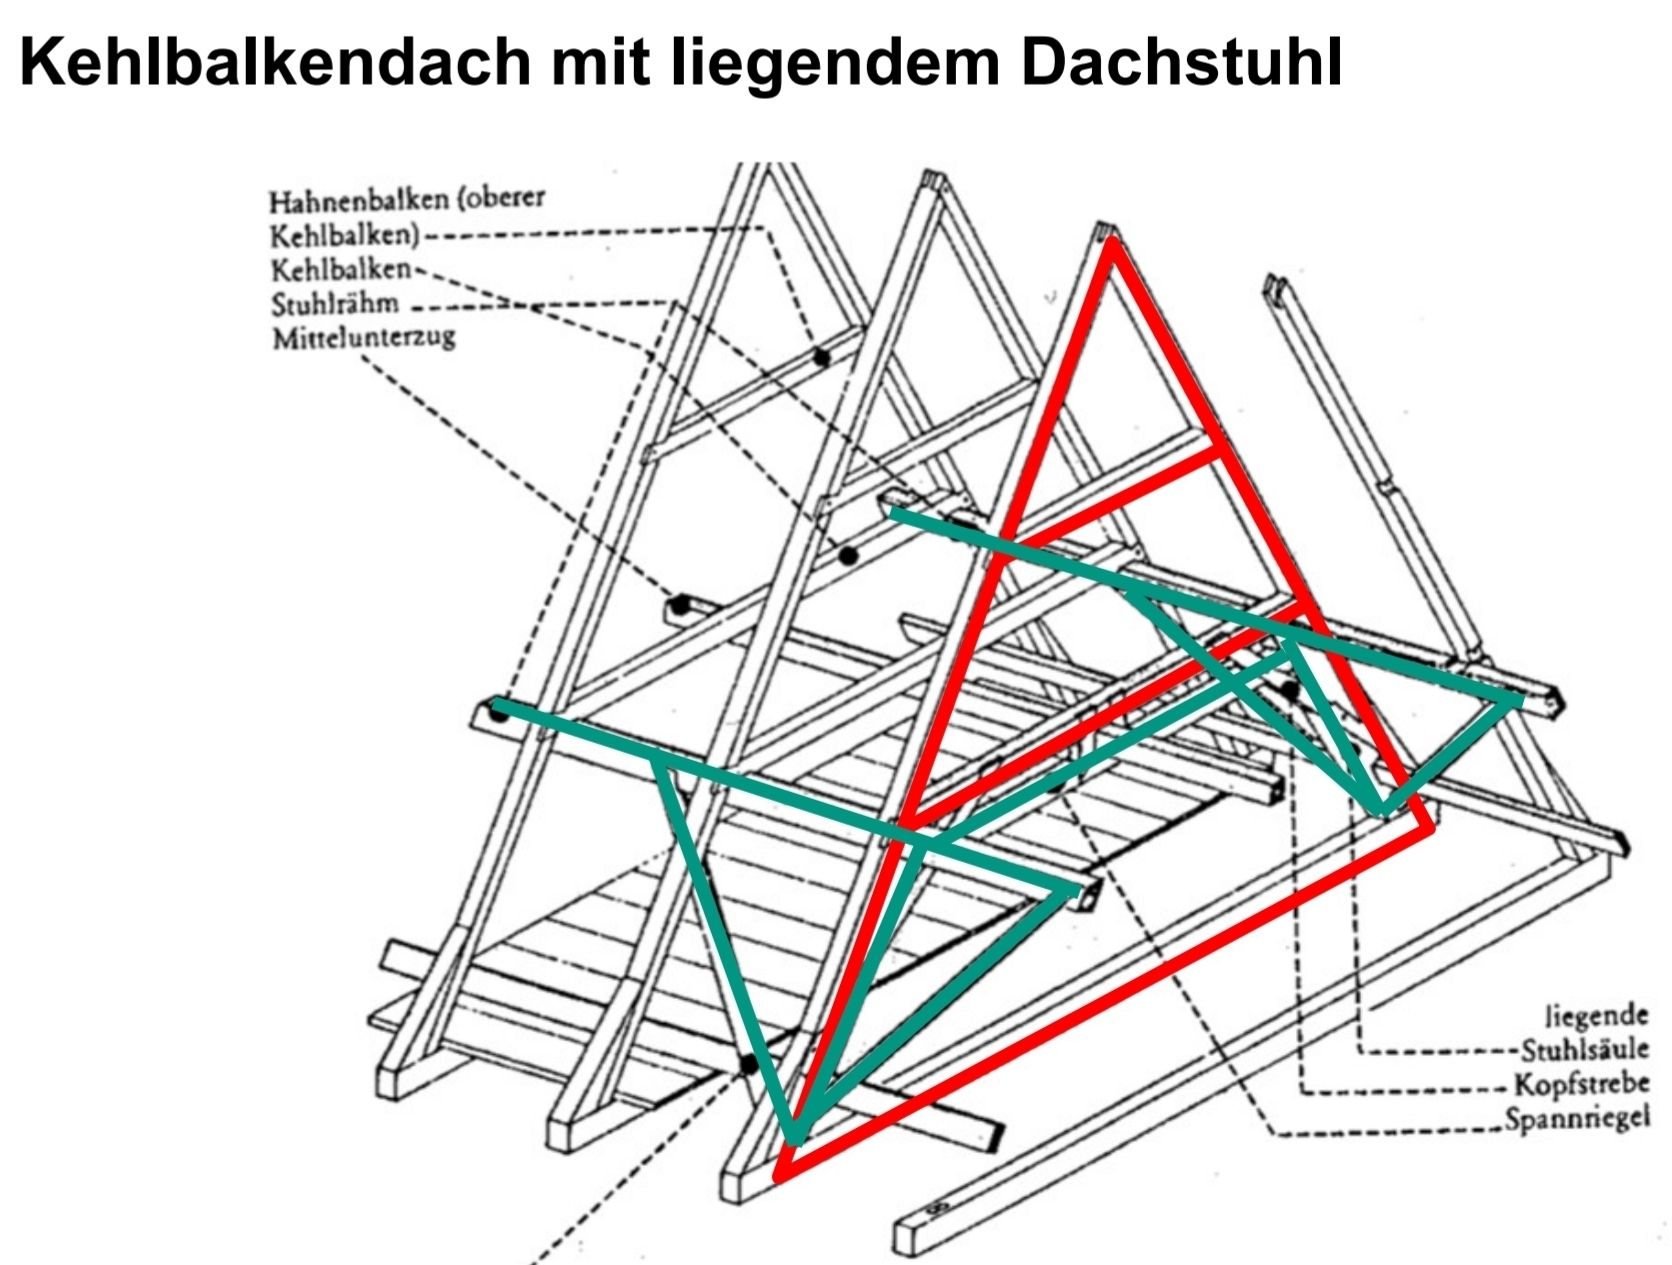
\includegraphics[width=0.45\textwidth]{Grafiken/Daecher/Liegender Stuhl Kehlbalkendach.jpg}
    \subsection{Hängewerk:}
            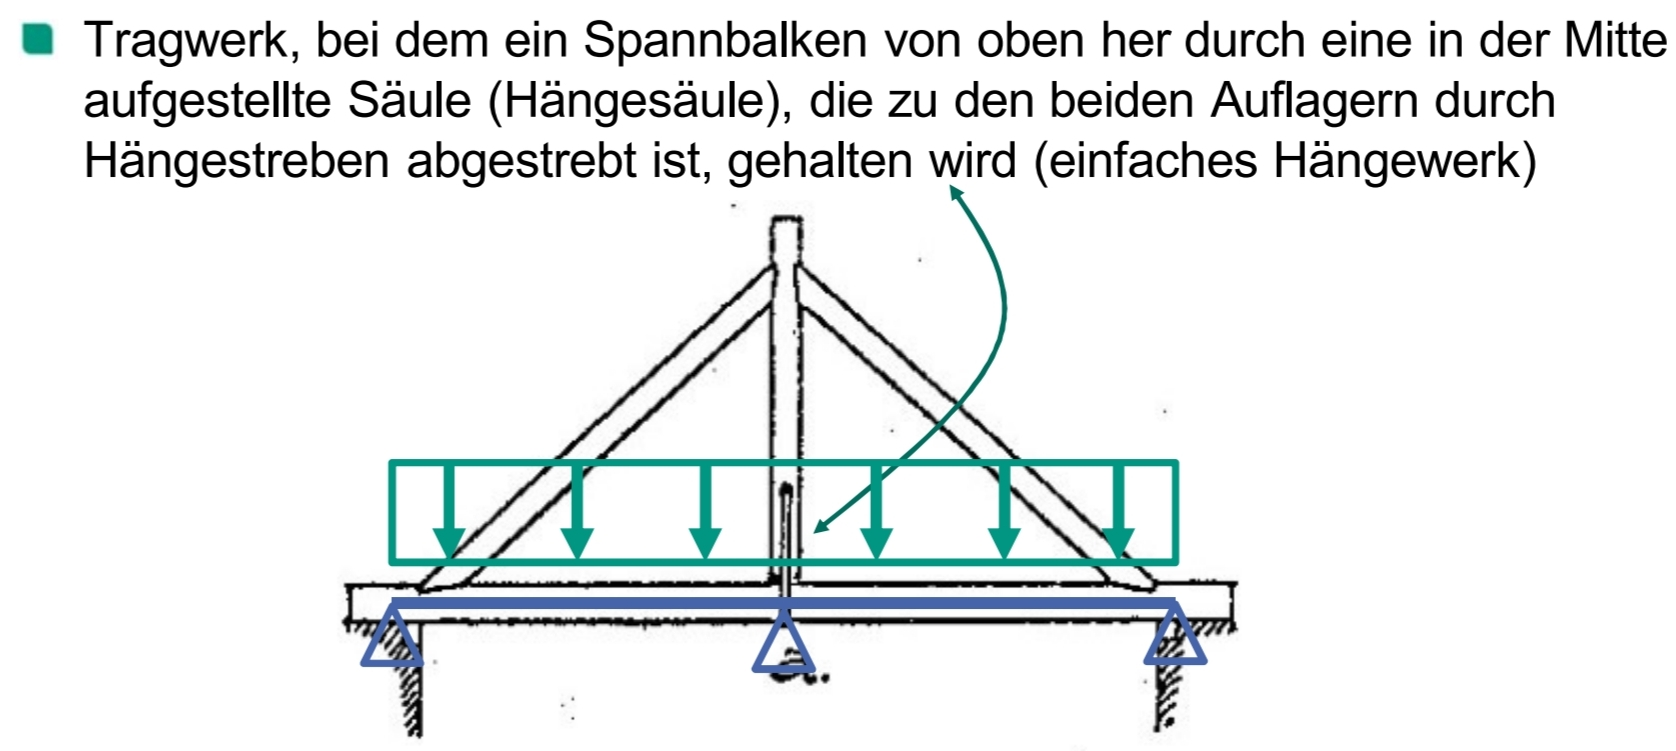
\includegraphics[width=0.45\textwidth]{Grafiken/Daecher/Haengewerk.jpg}
            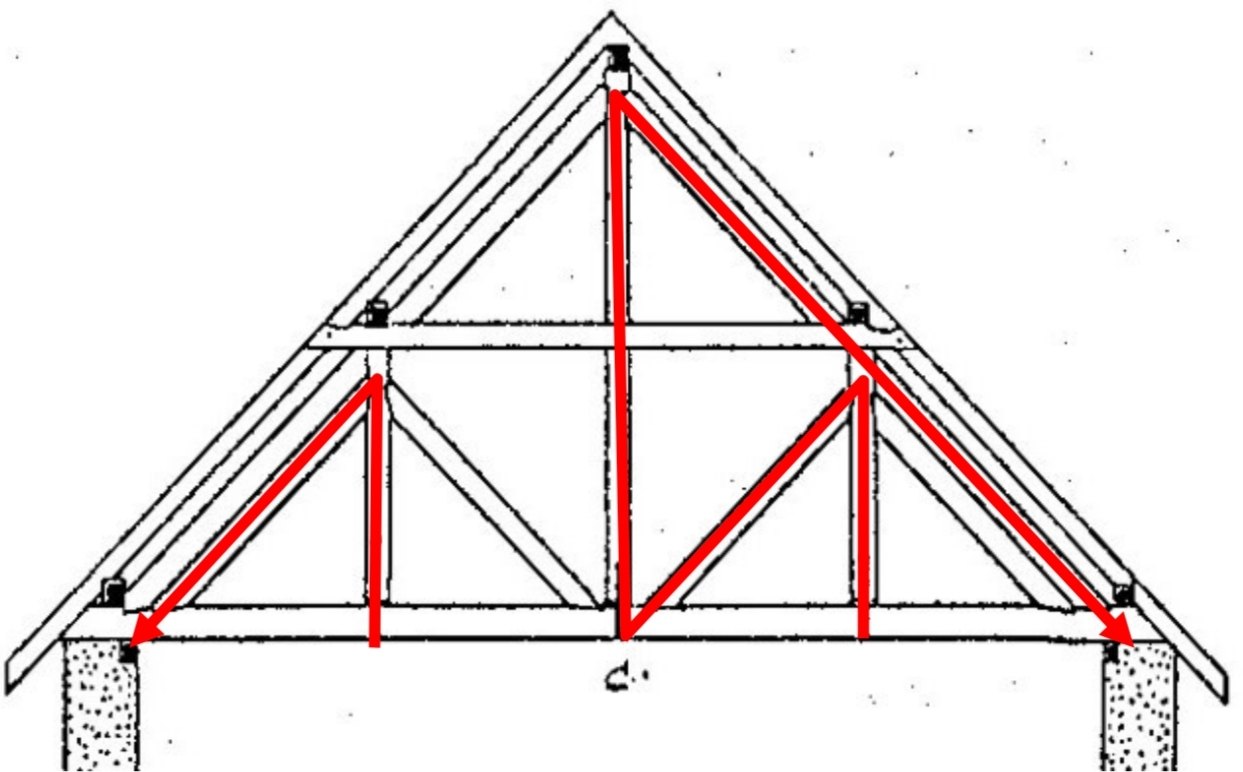
\includegraphics[width=0.45\textwidth]{Grafiken/Daecher/Mehrfaches Haengewerk.jpg}\\
            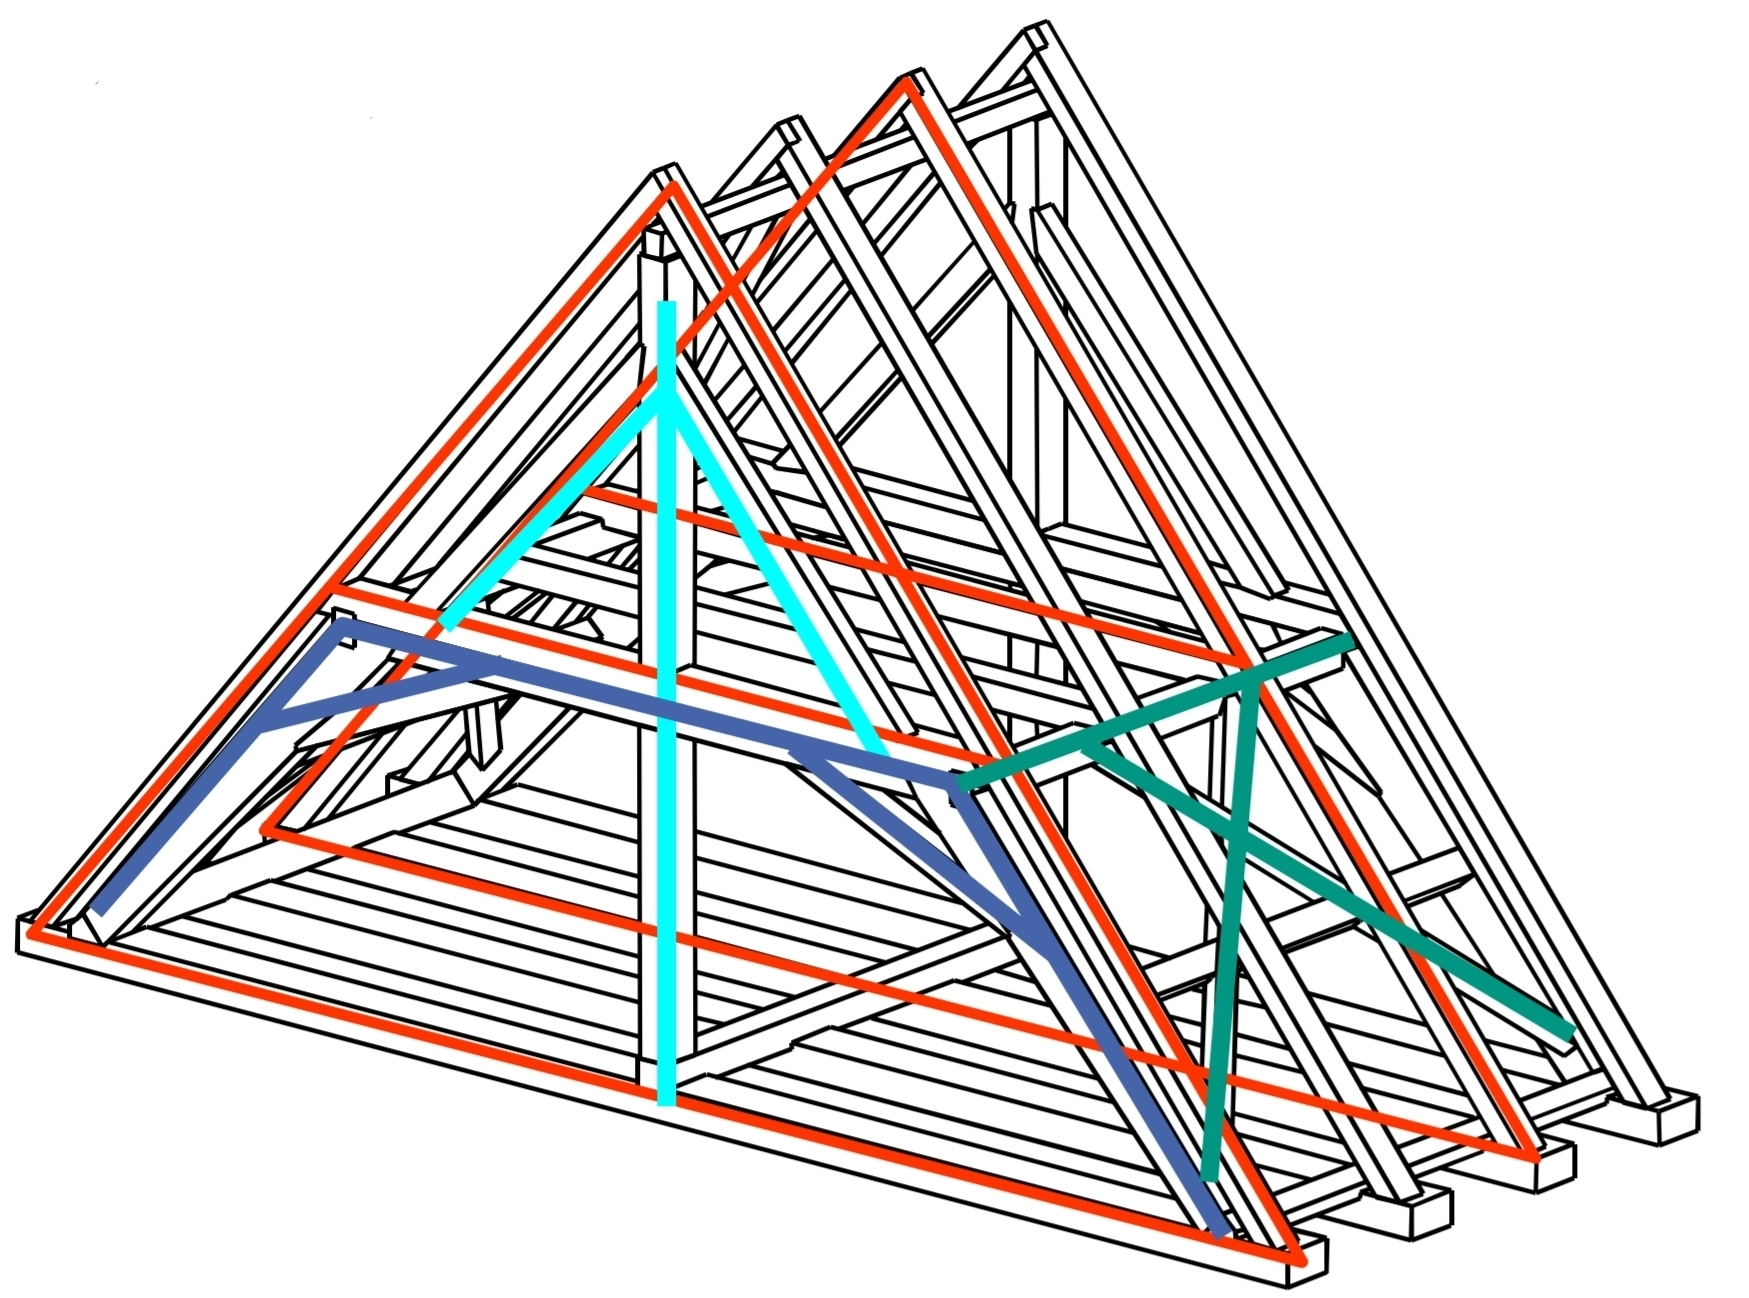
\includegraphics[width=0.45\textwidth]{Grafiken/Daecher/Haengewerk auf liegenden Stuhl.jpg}
            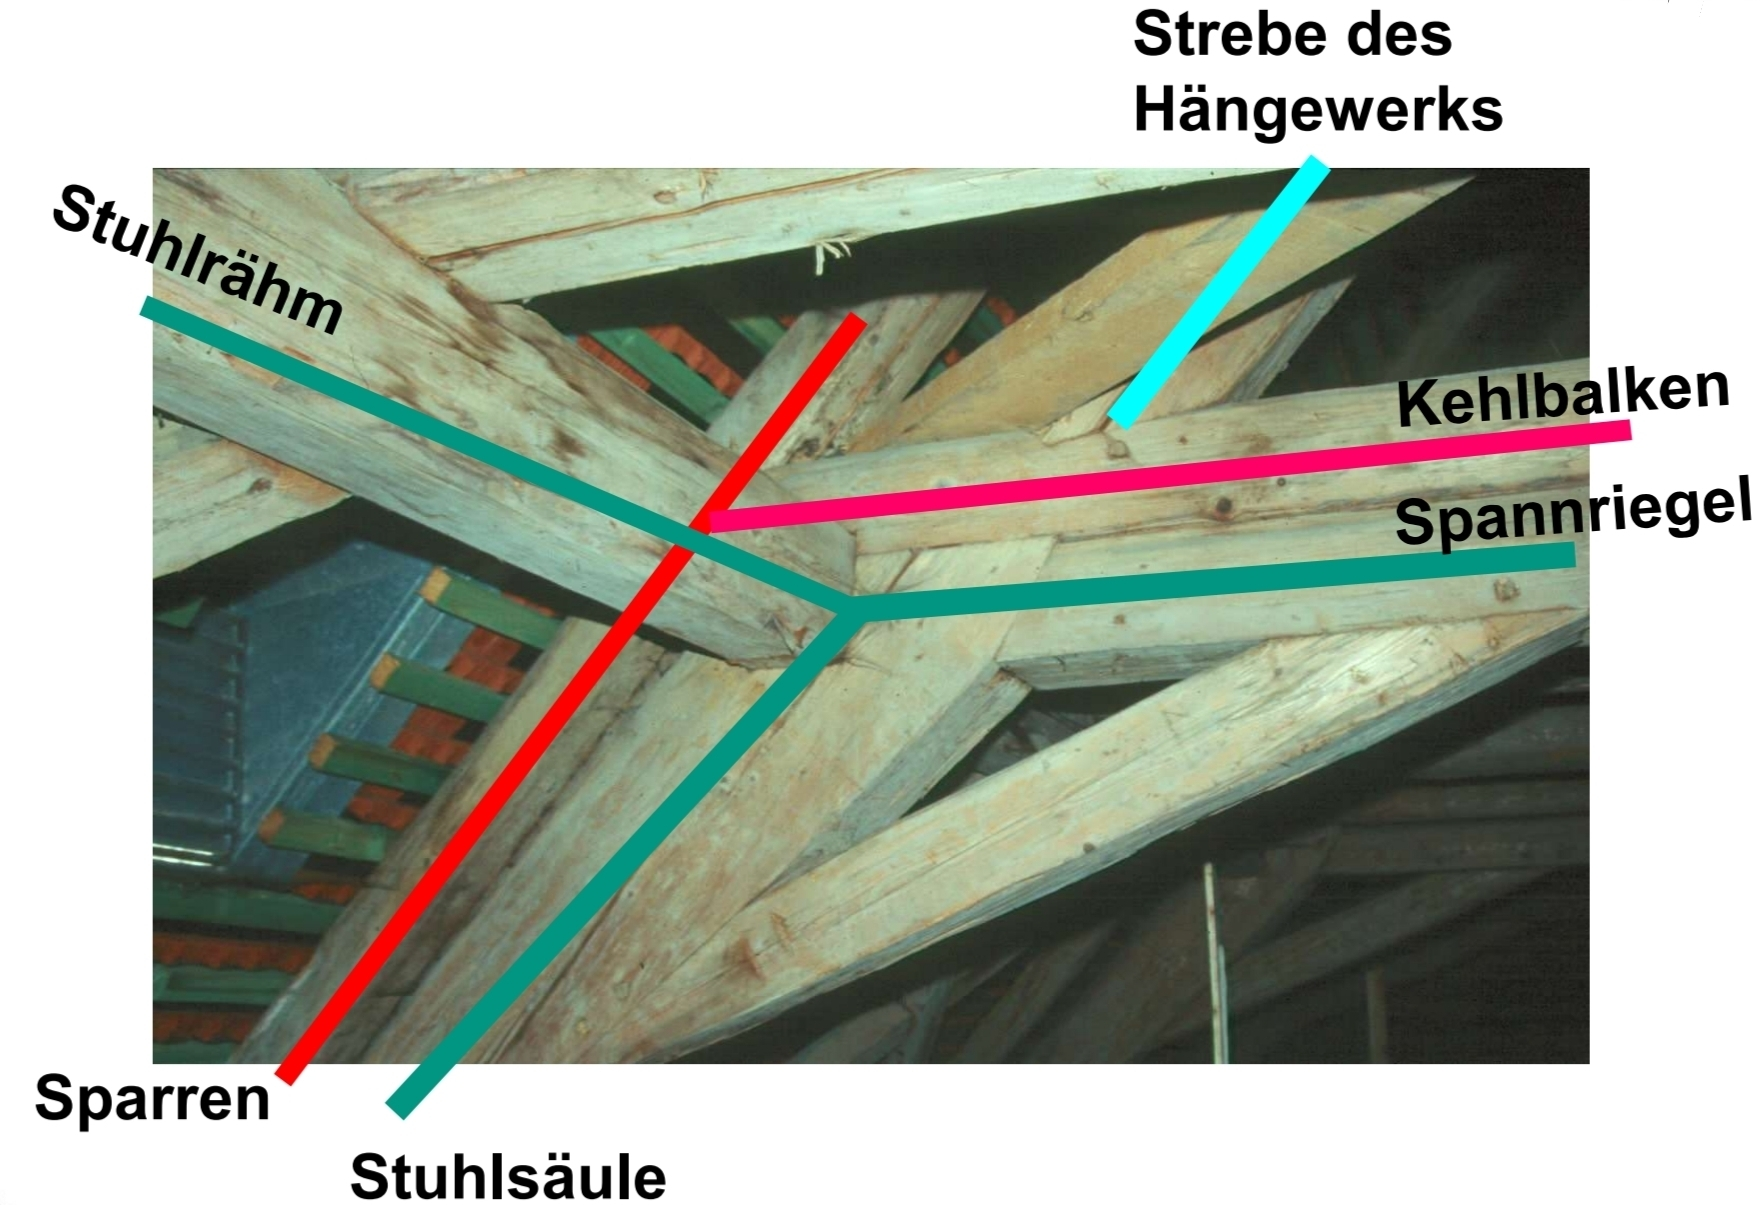
\includegraphics[width=0.45\textwidth]{Grafiken/Daecher/Knotenpunkt Haengewerk.jpg}\\
            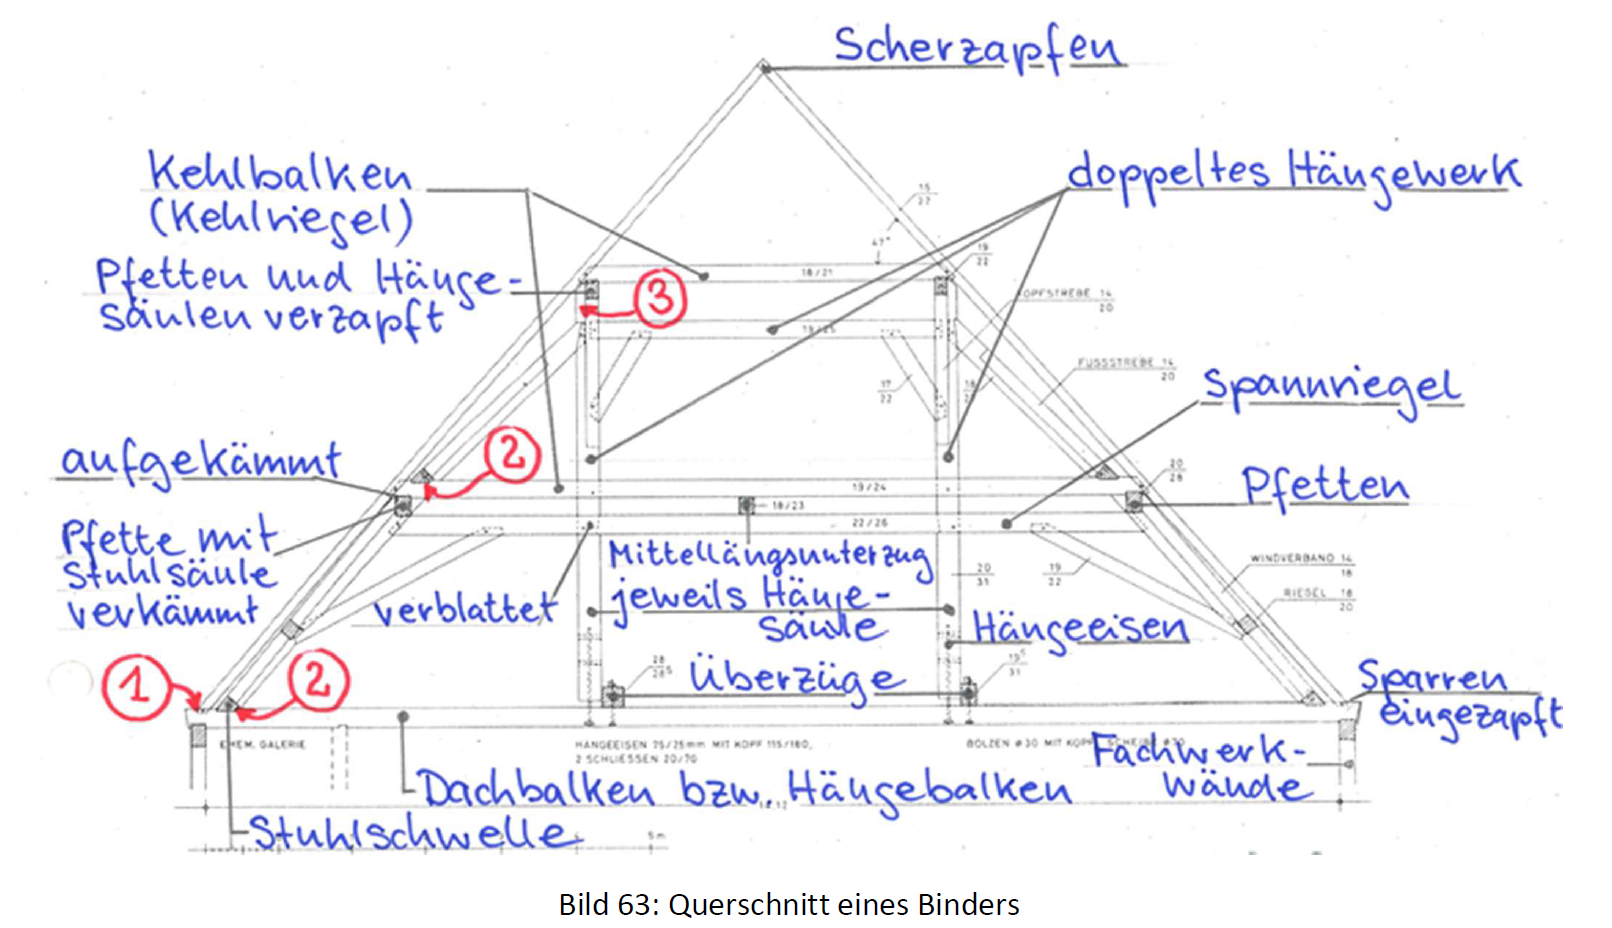
\includegraphics[width=0.45\textwidth]{Grafiken/Daecher/Dach kompliziert.png}
            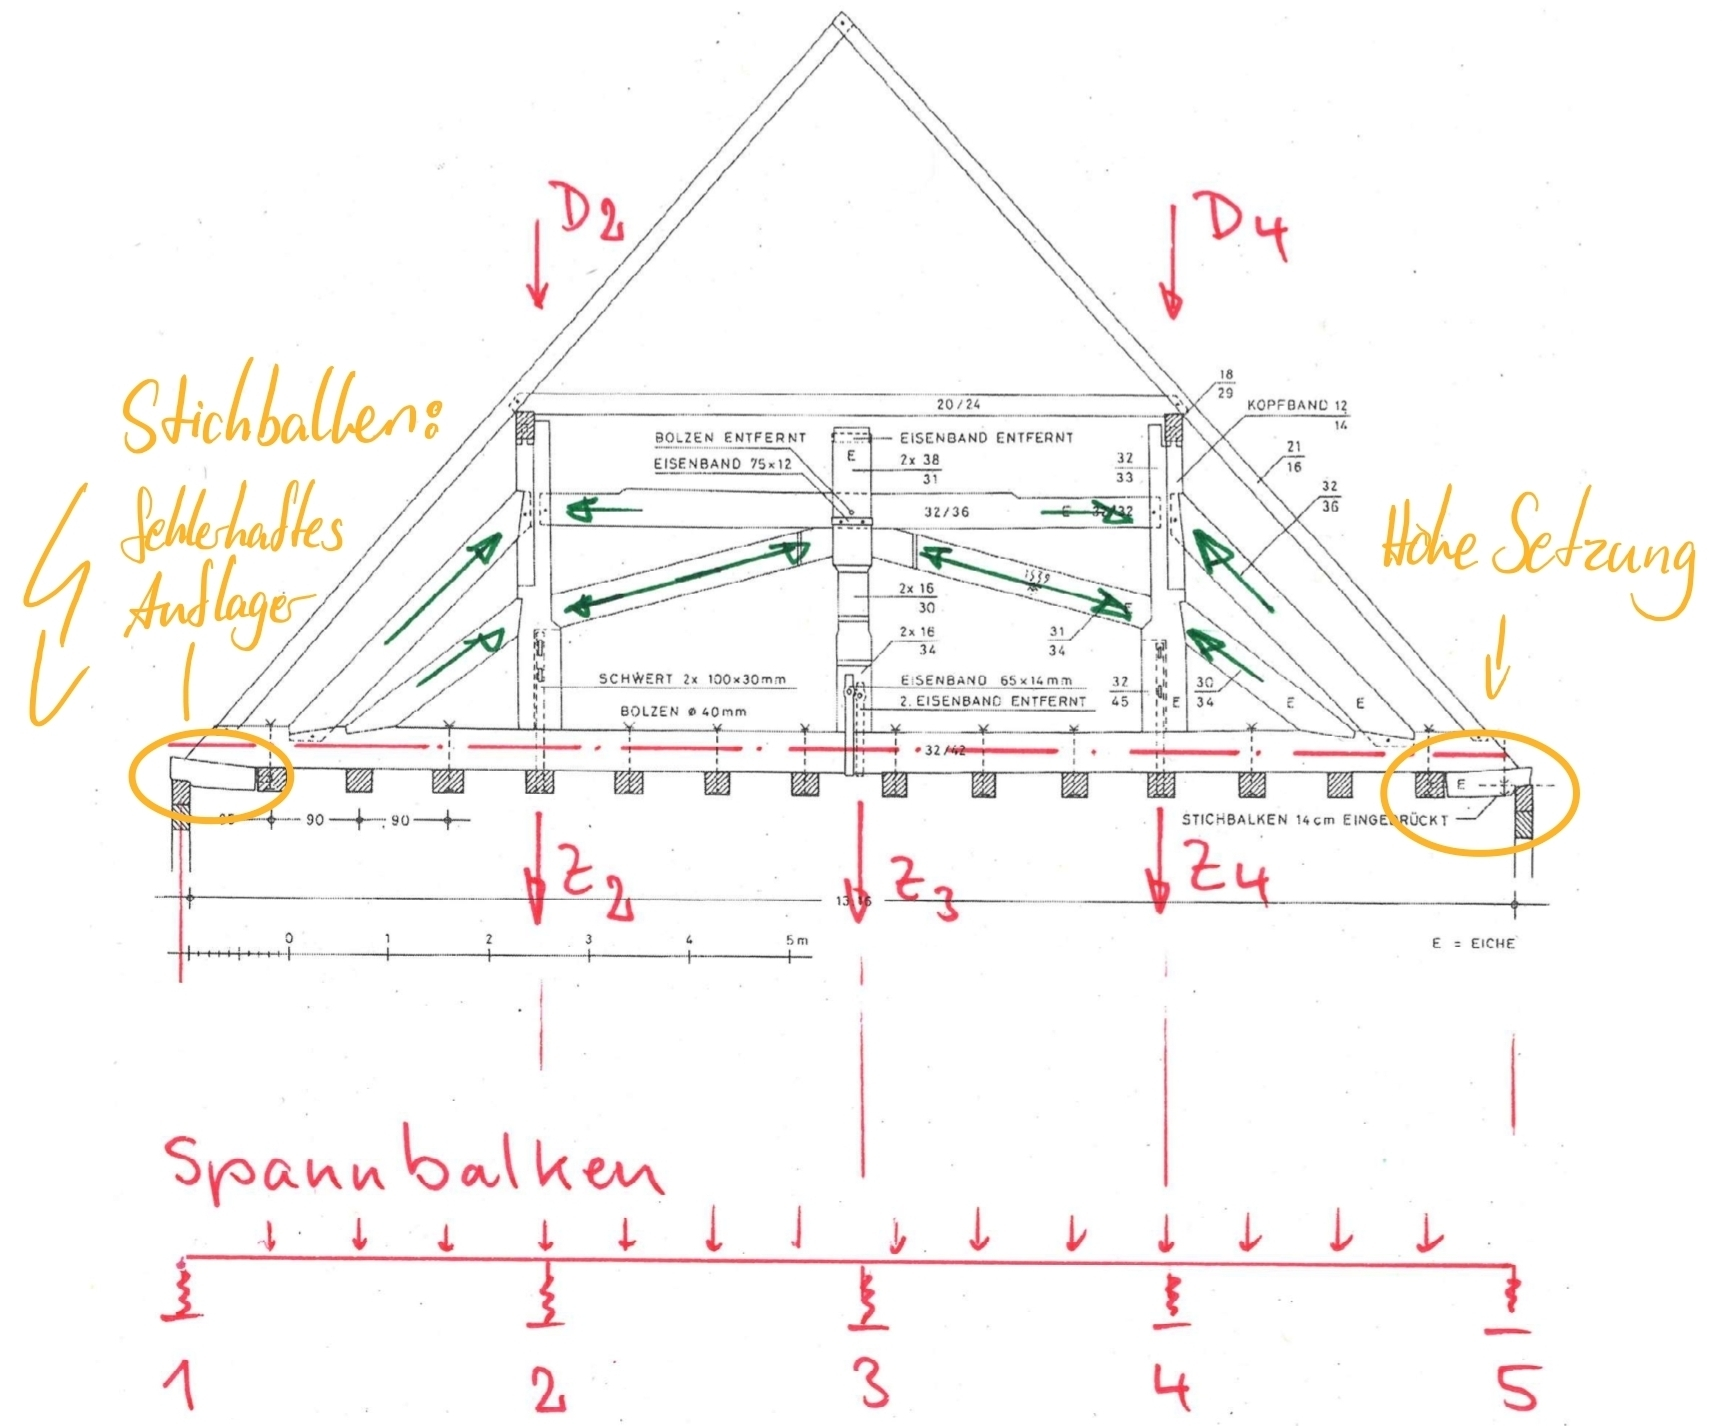
\includegraphics[width=0.45\textwidth]{Grafiken/Daecher/Fehlerhafter Stichbalken.jpg}
    \subsection{Binder Gespänne Abbund:}
            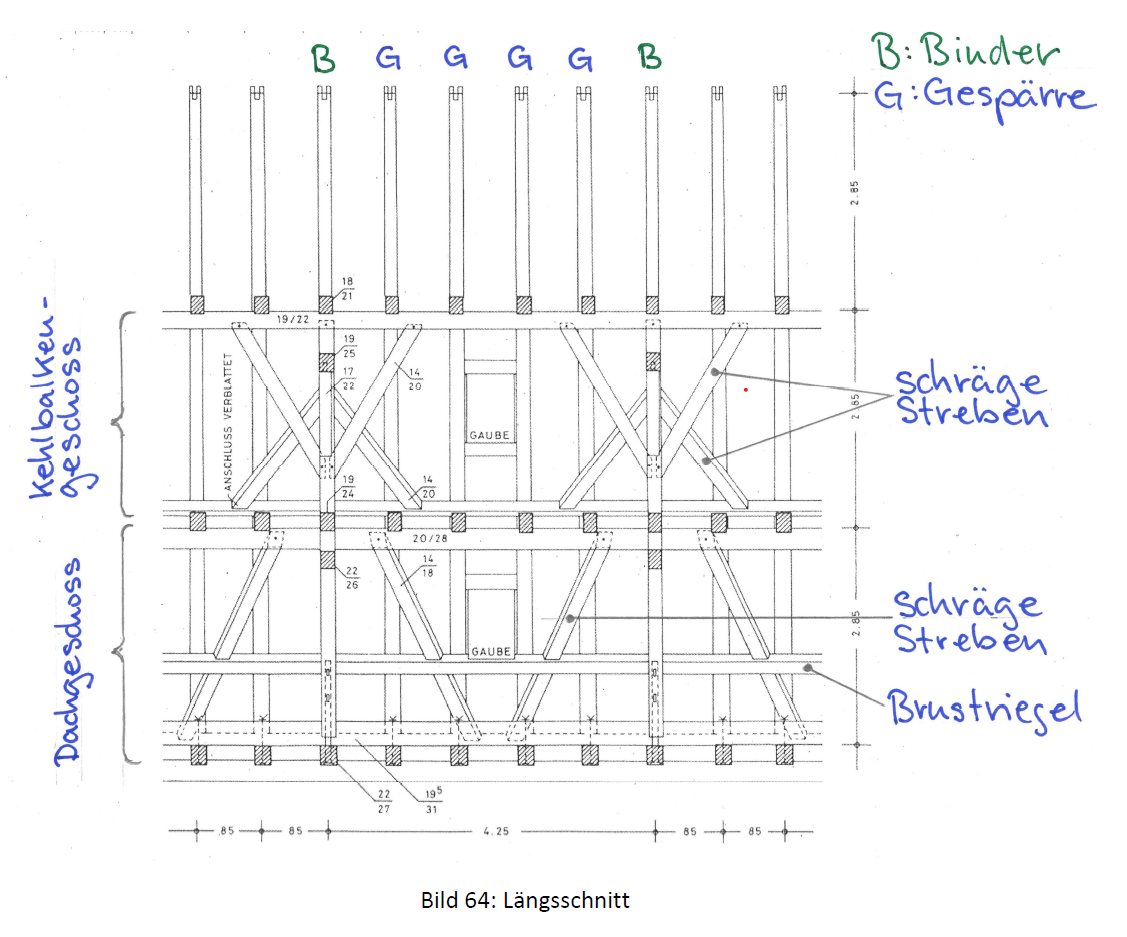
\includegraphics[width=0.45\textwidth]{Grafiken/Daecher/Binder Gespaenne Abbund.png}

    \subsection{Wirkende Kräfte markieren}
    
    \subsubsection{Beispiel 1: Howe'scher Träger}
        \begin{minipage}{0.6\textwidth}
            \begin{itemize}
                \item Bei dem Versuch die gesamte Auflagerkraft von 1,5·F der ersten steigenden und ersten fallenden Diagonale anteilig zuzuweisen, stellt sich die Frage, wie groß die jeweiligen Anteile sind (Bild 66, oben).
                \item Sieht man im Gesamtsystem einen Fachwerkträger mit steigenden (Bild 66, Mitte) und einen Fachwerkträger mit fallenden Diagonalen (Bild 66, unten), die sich aufgrund ähnlicher Steifigkeiten zu gleichen Teilen am Lastabtrag beteiligen, ist es naheliegend, die Belastung paritätisch auf beide Systeme aufzuteilen.
                \item Sodann kann man sich vom linken oder rechten Auflager kommend durch die Berechnung der einzelnen Stabkräfte hangeln (Bild 67).
            \end{itemize}
        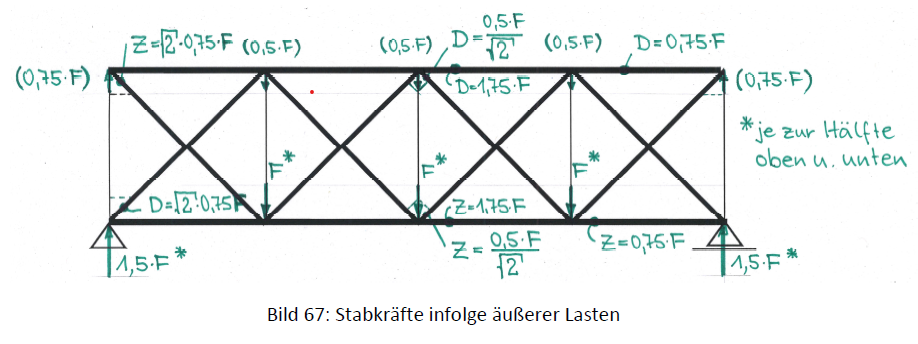
\includegraphics[width=1\textwidth]{Grafiken/Beurteilen alter Holzkonstruktionen/Kraftfluesse/Howescher Traeger - Ueberlagerte Stabkraefte.png}
        \end{minipage}
        \begin{minipage}{0.4\textwidth}
            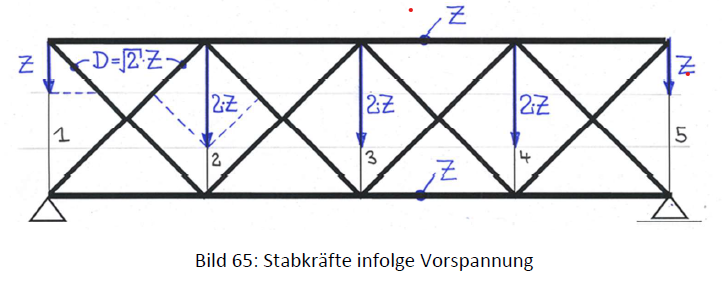
\includegraphics[width=0.95\textwidth]{Grafiken/Beurteilen alter Holzkonstruktionen/Kraftfluesse/Howescher Traeger - Vorspannung.png}\\
            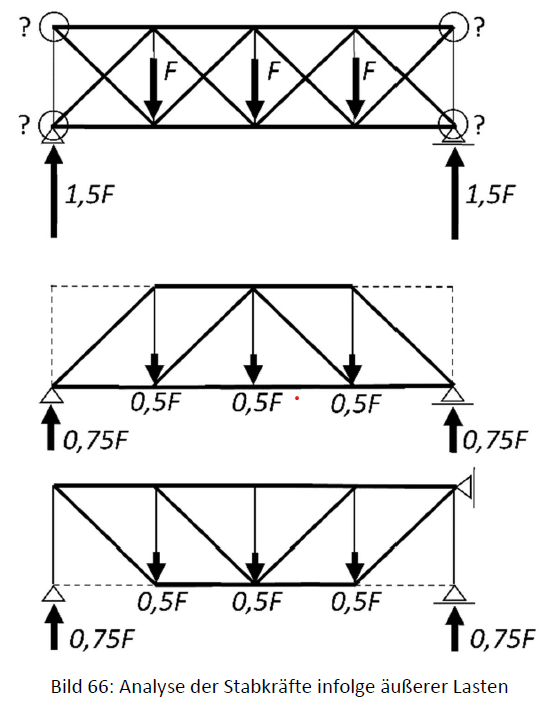
\includegraphics[width=0.95\textwidth]{Grafiken/Beurteilen alter Holzkonstruktionen/Kraftfluesse/Howescher Traeger - Aussere Lasten.png}
        \end{minipage}
        
    \subsubsection{Beispiel 2: Kräftespiel in Schwalbenschwanzverbindungen}
        \begin{minipage}{0.5\textwidth}
            \begin{itemize}
                \item Die Kontaktkräfte (bzw. -spannungen) in den beiden Fugen wirken zwischen den Schwalbenschwanzflanken (in Rot) und den jeweiligen Innenkanten der Blattsassen (in Grün). 
                \item Zunächst sei ein Punkt (in Rot) auf der Wirkungslinie von $F$ etwa auf halber Länge des Blattes festgelegt. Die Wirkungslinien von $D_1$ und $D_2$ kreuzen sich darin. Ihre Neigung bezüglich der Fugen sei dabei so eingestellt, dass von grundsätzlich unterschiedlichen Reibungswinkeln $\varphi$ ausgegangen wird. 
                \item Das illustrierte Kräftespiel ist so entworfen, dass der angeblattete Stab frei von Momenten ist.
            \end{itemize}
        \end{minipage}
        \begin{minipage}{0.5\textwidth}
            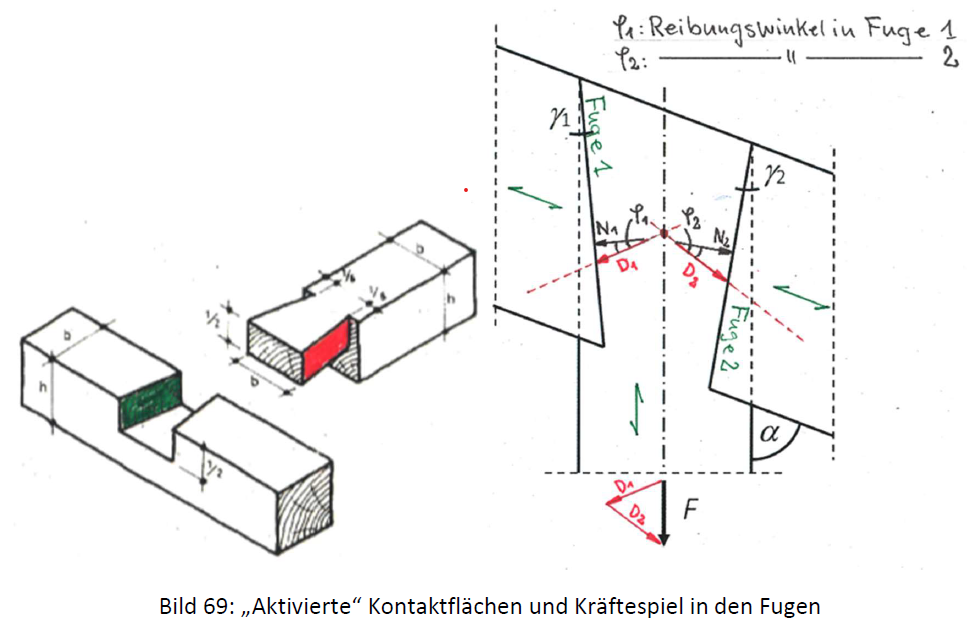
\includegraphics[width=0.95\textwidth]{Grafiken/Beurteilen alter Holzkonstruktionen/Kraftfluesse/Kraeftespiel in Schwalbenschwanzverbindungen.png}
        \end{minipage}    
        
    
\newpage
\section{Beurteilen alter Holzkonstruktionen}

    \subsection{Allgemeines:}
        Beurteilung alter Holzkonstruktion oder lokal begrenzten Bereiche, in Normen festgeschriebenen Beanspruchbarkeiten auf vorgefundenen Bauteile übertragen. Übertragbarkeit sichergestellt, ...
        \begin{itemize}
            \item z. B. indem Querschnittswerte, den Festlegungen in Sortiernormen entsprechen.
                \begin{itemize}
                    \item $\rightarrow$ Falls nicht gegeben $\rightarrow$ besondere Überlegungen. Beispielhafte Aspekte:
                \end{itemize}
            \item Berücksichtigung Fehlstellen infolge Wurmfraß oder Pilzbefall bzw. Fäulnis
            \item Berücksichtigung von Rissen durch Schubtragfähigkeit
            \item Querschnittsnachweise mit Nettoquerschnitten, d. h. Abzug von Zapfenlöchern, Aussparungen, Bohrungen u.v.a.m.
        \end{itemize}
        
        Entscheidende Frage, wie flächendeckend eine Zustandsuntersuchung durchgeführt wird und wo Vereinfachungen möglich sind. Lösungsansätze hierzu:
        \begin{itemize}
            \item Untersuchungsergebnisse auf nicht untersuchte Bereiche übertragen, falls angemessene Zuverlässigkeit gegeben .
            \item Identifikation von Bauteilbereichen, die stark beansprucht sind oder neuralgische Stelle einer alten Holzkonstruktion, Intensivierung der Untersuchungen in diesen Bereichen
            \item Identifikation von Bauteilbereichen, aus Erfahrung häufig Probleme mit Pilz- und Insektenbefall
        \end{itemize}
        
        Untersuchungen für Beurteilung
        \begin{itemize}
            \item unmittelbar sichtbaren
                \begin{itemize}
                    \item können visuell wahrgenommen werden
                \end{itemize}
            \item verdeckten Schäden
                \begin{itemize}
                    \item besonderes Instrumentarium nötig
                    \item bedingen immer das Schaffen eines speziellen Zugangs zum Schadensherd (konstruktiver Eingriff)
                \end{itemize}
        \end{itemize}
        
    



    \subsection{Vorgehensweise Untersuchung altes Tragwerk:}
        \begin{itemize}
            \item Die Festigkeit eines Bauteiles aus Holz wird im wesentlichen durch zwei Faktoren beeinflußt:
                \begin{itemize}
                    \item Die Holzstruktur des sog. fehlerfreien Holzes, die sich zum Beispiel durch Jahrringbreite und/oder Rohdichte beschreiben läßt
                    \item Die sogenannten Holzfehler, die innerhalb eines Bauteils zwangsläufig auftreten. Einige wesentliche Holzfehler sind die Ästigkeit, der von der Bauteillängsachse abweichende Faserverlauf sowie Risse und Pilz- bzw. Insektenbefall. Dabei ist zu beachten, daß sich Holzfehler auf die verschiedenen Festigkeiten (Biege-, Druck-, Zug-, Scherfestigkeiten) in den zwei Hauptrichtungen des Holzes (parallel und rechtwinklig zur Faser) deutlich unterschiedlich auswirken können.
                \end{itemize}
        \end{itemize}
        
    \subsection{Bohrwiderstandsmessungen}
        \begin{minipage}{0.55\textwidth}
        Die Bohrwiderstandsmessung ist ein Verfahren, bei dem ein Holzbauteil mit einer dünnen Bohrnadel
        und einer konstanten Vorschubgeschwindigkeit durchbohrt wird. Ein Prozessor im Gerät wandelt die
        Leistungsaufnahme des Motors in einen Bohrwiderstand um, der über dem Bohrweg aufgetragen wird.\\
        In einem etwa 15 cm dicken Pfosten, an dem seitlich rechts eine Strebe auftrifft, wurde an der mit
        einem Fadenkreuz gekennzeichneten Stelle eine zur Oberfläche der Pfostenseite rechtwinklig ausgerichtete
        Bohrwiderstandsmessung vorgenommen.
        \end{minipage}
        \begin{minipage}{0.45\textwidth}
        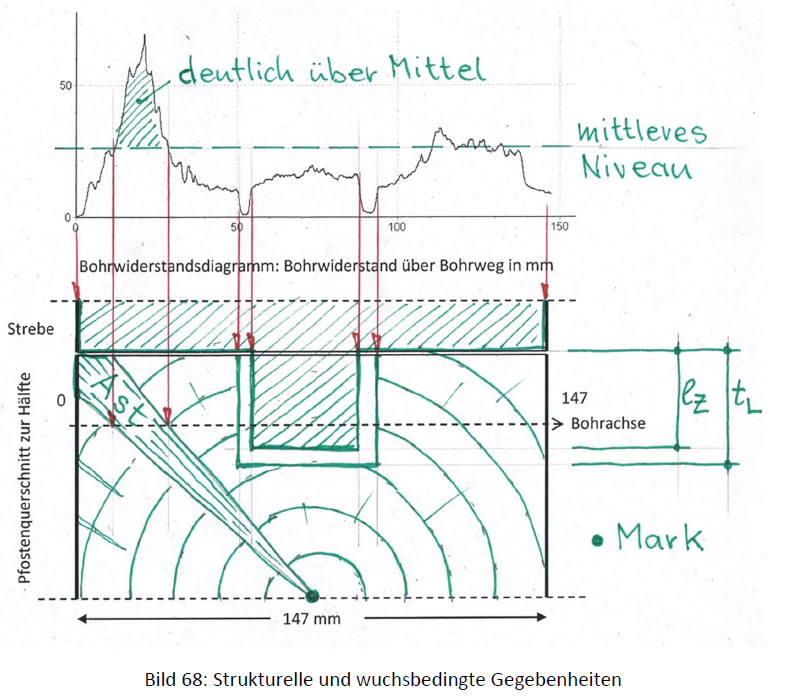
\includegraphics[width=1\textwidth]{Grafiken/Beurteilen alter Holzkonstruktionen/Bohrwiderstandsmessung.png}
        \end{minipage}


    \subsection{Visuelle Holzsortierung nach DIN4074-1:}
        \begin{itemize}
            \item Beispiele: Skript S.45
            \item Sortierklasse bestimmen:
                \begin{itemize}
                    \item Astdurchmesser
                    \item Faserneigung
                    \item Risstiefe
                \end{itemize}
            \item Durch visuelle Sortierung erreichbare Klassen:\\
                \begin{tabular}{|l|c|c|}
                \hline Holzart & Sortierklasse & Festigkeitsklasse \\
                \hline Fichte, Tanne, & S 7, S 7K & C 16 \\
                        Kiefer, Lärche, & S 10, S 10K & C 24 \\
                        Douglasie & S 13, S 13K & C 30 \\
                \hline Eiche & LS 10, LS 10K & D 30 \\
                \hline Buche & LS 10, LS 10K & D 35 \\
                         & LS 13, LS 13K & D 40 \\
                \hline
                \end{tabular}
            \item Holzfeuchte $\overset{!}{=} 20 \%$
            

            \item Risse
                \begin{itemize}
                    \item Risstiefe wird an 3 Punkten ($t_1,t_2,t_3$) gemessen (siehe Bild links)
                    \item $R=\frac{r_1}{b} \quad$ bzw. $\quad R=\frac{r_1+r_2}{b}$
                \end{itemize}
        \end{itemize}
                
                \resizebox{0.8\textwidth}{!}{\begin{tabular}{llll}
                \hline Sortierklasse & S 7, S 7K & S 10, S 10K & $S 13, S 13 K$ \\
                \hline $\cdot$ Blitzrisse, Ringschäle & nicht zulässig & nicht zulässig & nicht zulässig \\
                \hline $\cdot$ Schwindrisse & $R \leq 3 / 5$ & $R \leq 2,5 / 5 $ & $R \leq 2 / 5$ \\
                \hline
                \end{tabular}}
                
                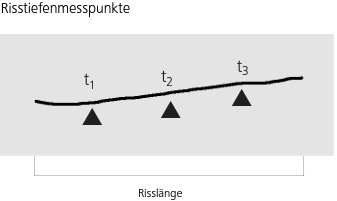
\includegraphics[width=0.3\textwidth]{Grafiken/Beurteilen alter Holzkonstruktionen/Visuelle Holzsortierung nach DIN4074-1/Risstiefenmesspunkte.png}
                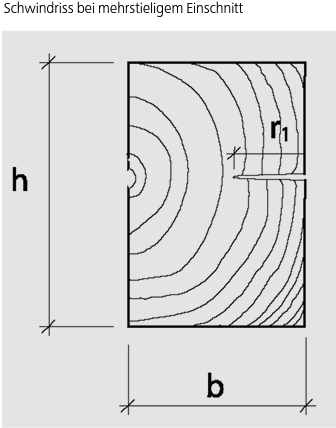
\includegraphics[width=0.3\textwidth]{Grafiken/Beurteilen alter Holzkonstruktionen/Visuelle Holzsortierung nach DIN4074-1/Schwindrisse bei mehrstieligem Einschnitt.png}
                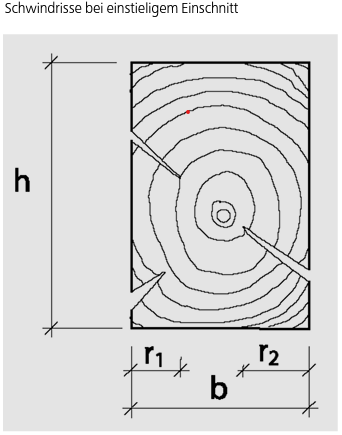
\includegraphics[width=0.3\textwidth]{Grafiken/Beurteilen alter Holzkonstruktionen/Visuelle Holzsortierung nach DIN4074-1/Schwindrisse bei einstieligem Einschnitt.png}
        \begin{itemize}
            \item Biegenachweis Bauteil Bestand nicht eingehalten?\\
                $\rightarrow$ Visuelle Begutachtung um Sortierklassen zu erhöhen, tatsächliche Festigkeit/Holzklasse möglicherweise höher als in Statik vorgeschrieben
        \end{itemize}   

    
    
    \subsection{Gefährdung durch holzzerstörende Pilze}
        \subsubsection{Allgemeines zur Gefährdung durch holzzerstörende Pilze} 
        Pilzwachstum erst wenn freies Wasser in Zellhohlräumen; Holzfeuchte $u$ oberhalb Fasersättigungsbereiches $\hateq$ in etwa $u\leq 30 \%$ (grober Mittelwert für die einheimischen Nadelhölzer)\\ 
        Fasersättigung bei vorhandenen Temperatur erreicht wenn Holz langfristig relativen Feuchte $\varphi=100 \%$ ausgesetzt\\  Freies Wasser wenn zusätzliches Wasserangebot vorliegt, z.B. durch Beregnung oder durch Tauwasserbildung im Querschnitt.\\
        Aus Sicherheitsgründen (Streuung d. Eigenschaften) messen Holzfeuchte an jeder Stelle mit Einzelmessung (z.B. mit Einschlagelektrode und möglichst an ungünstig erscheinender Stelle, hier mit $u_1$ bezeichnet) einen Wert $u_1 \leq 20 \%$ \\
        messen $\rightarrow$ Pilzwachstum vermieden, wenn Zustand dauerhaft gegeben.\\
    
        Ausgabe 1990 von DIN 68 800-3 zugrunde gelegten 'Insekten-Philosophie':\\ 
        Befall durch Insekten toleriert, wenn  Schaden durch kontrollierbarkeit Holzes verhindert\\
        Analog Pilzbefall: zulässig, wenn zu keinem Schaden führt.\\
        $\rightarrow$ Solange Holzfeuchte an keiner Stelle den Wert $u=30 \%$ bzw. der Einzelwert $u_1=20 \%$ nicht länger als 6 Monate überschreitet, kann zwar eine Pilzspore zur Hyphe (feiner Zellfaden) auskeimen, aber noch keinen Schaden am Holz verursachen. Bei anschließender Unterschreitung dieser Feuchten wird der Pilz sein Wachstum wieder einstellen. (Anm.: Nach Abschn. $2.3 .2$ in DIN 68 800-3 besteht eine Gefahr durch Pilzbefall, wenn $\mathrm{u}_1=20 \%$ langfristi überschritten wird.)\\
        
        Echter Hausschwamm: Im fortgeschrittenen Stadium in der Lage, auch trockenes Holz zu befallen.\\
        Wie schnell trocknet zu feucht eingebautes oder nachträglich zu feucht gewordenes Holz auf die hinsichtlich des Pilzwachstums ungefährliche Feuchte $\mathrm{u}<30 \%$ oder $\mathrm{u}_1<20 \%$ herunter?:\\ 
        \subsubsection{Zusammenfassung der Untersuchungsergebnisse}
        Die Feuchteabgabe aus zu feuchtem Holz innerhalb eines Bauteils verläuft um so schneller, je diffusionsoffener die Bauteiloberfläche bezgl. Wasserdampf ausgebildet ist.

    
    \subsection{Begriffe:}
        \begin{itemize}
            \item Fäulnis, Fäule:\\
                - Zersetzung, Gärung, Verwesung organischer Stoffe
            \item Myzel, Myzelium:\\
                - Gesamtheit der Pilzfäden eines höheren Pilzes
            \item Fruchtkörper:\\
                - sowohl unterirdisch als auch oberirdisch wachsender Teil des Pilzes
        \end{itemize}
    
    \subsection{Holzpilze - Fakten:}
        \begin{itemize}
            \item Holzpilze häufigsten vorkommenden Bauholzschädlinge.
            \item Pilzsporen sind praktisch allgegenwärtig und wachsen unter günstigen Bedingungen zu einem Myzel heran.
            \item Was sind die Bedingungen für die Entwicklung?\\
            - Feuchte/Nährboden/Sauerstoff/Temperatur
            \item Pilze scheiden wasserlösliche Enzyme aus und zerlegen damit die organischen Moleküle des Holzes.
            \item Neue Sporen werden im Fruchtkörper erzeugt.
        \end{itemize}
        
    \subsection{Pilzwachstum:}
        \begin{itemize}
            \item Wichtigstes Kriterium für Pilzwachstum ist die Feuchte des Nährbodens
            \item Pilzbefall, wenn die Holzfeuchte über Fasersättigung liegt (freies Wasser)
            \item Auf trockenem Holz ist kein Pilzwachstum möglich.
            \item Auf wassergesättigtem Holz ist kein Pilzwachstum möglich
        \end{itemize}
        
    \subsection{Grenzzustände der Holzfeuchte:}
        \begin{itemize}
            \item Darrtrocken $\leftrightarrow$ Fasersättigung $\leftrightarrow$ Wassersättigung
        \item Holzfeuchte $u=0 \%$\\
            $\rightarrow$ Es ist kein Wasser im Holz enthalten.
        \item $u \pm 28 \%$
            \begin{itemize}
                \item Das gesamte Hohlraumsystem in den Zellwänden ist mit Wasser gefüllt.
                \item Der prozentuale Wert der Fasersättigung hängt im Einzelnen von der Holzart ab.
            \end{itemize}
        \end{itemize}
                
        
    \subsection{Pflanzliche und tierische Holzschädlinge}

        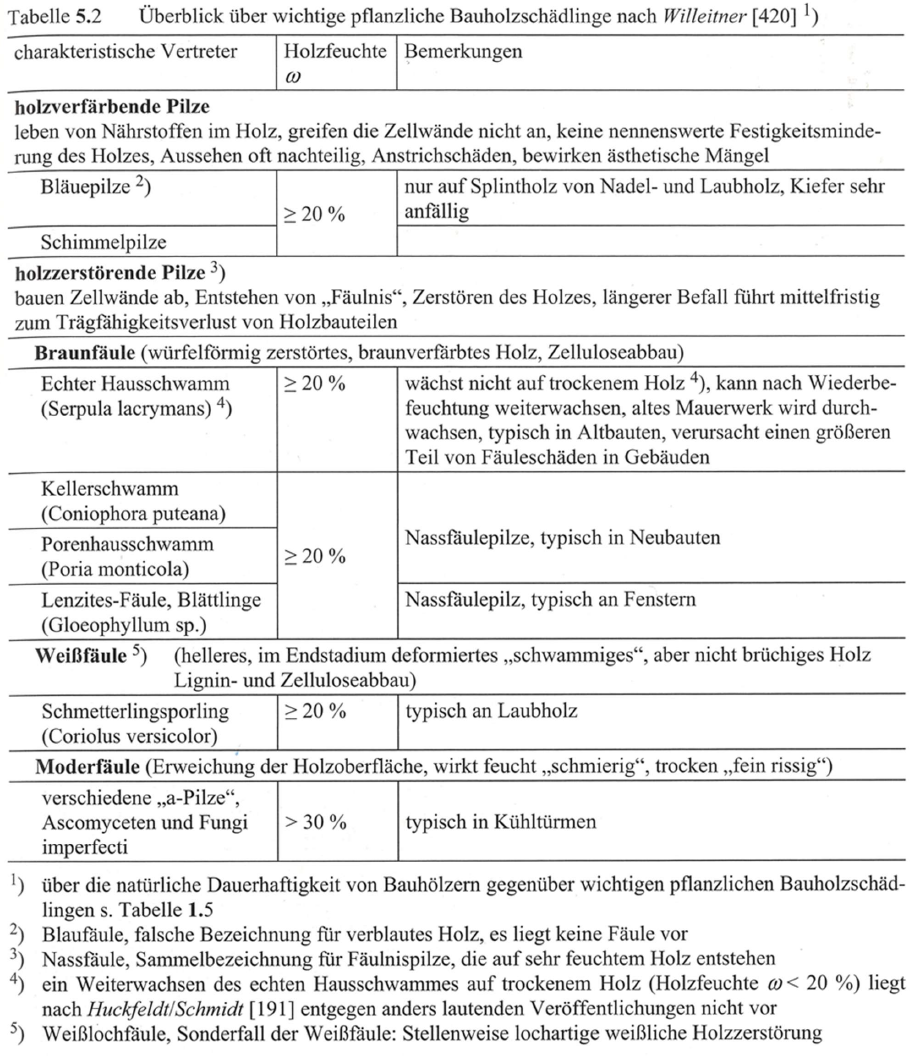
\includegraphics[width=0.5\textwidth]{Grafiken/Beurteilen alter Holzkonstruktionen/Holzschädlinge/Pflanzliche Holzschaedlinge.png}
        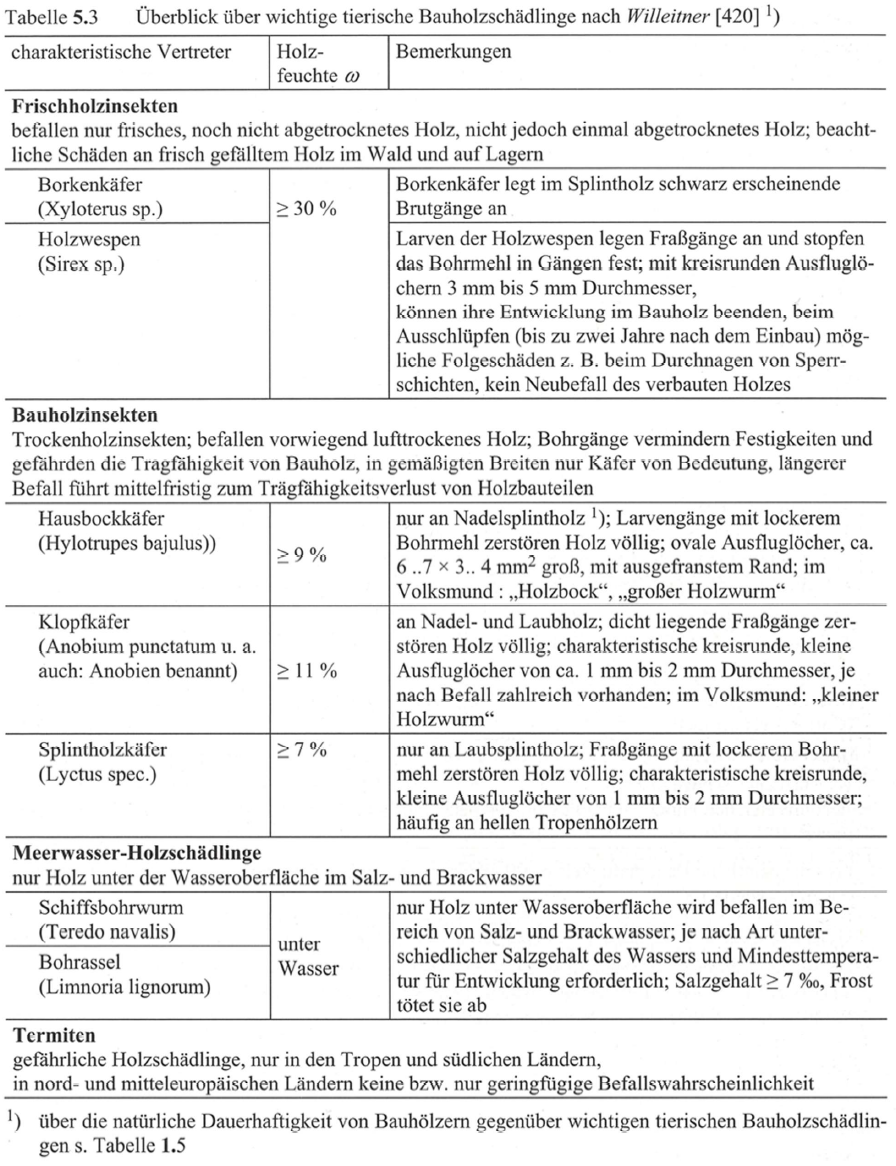
\includegraphics[width=0.5\textwidth]{Grafiken/Beurteilen alter Holzkonstruktionen/Holzschädlinge/Tierische Holzschaedlinge.png}
        
    \subsection{Holzinsekten}
        \begin{itemize}
            \item Frischholzinsekten
                \begin{itemize}
                    \item Sie benötigen hohe Holzfeuchten und befallen daher lebende Bäume und frisch geschlagenes Holz.
                    \item  Forstschädlinge gefährden die Gesundheit des Baumes/Waldes.
                    \item  Technische Schädlinge entwerten das Holz stehender oder gefällter Bäume.
                    \item  Scheibenböcke, Borkenkäfer, Fichtensplintböcke, Holzwespen, Kernholzkäfer
                \end{itemize}
            \item Trockenholzinsekten
                \begin{itemize}
                    \item Sie entwickeln sich auch bei geringer Holzfeuchte und befallen verbautes Holz.
                    \item Sie sind die eigentlichen Bauholzschädlinge.
                \end{itemize}
        \end{itemize}
        
    \subsection{Einige Fakten}
        \begin{itemize}
            \item In unserem Klimagebiet sind Käfer die wichtigsten Trockenholzinsekten.
            \item Käferlarven zerkleinern und fressen (teilweise) das Holz. $\rightarrow$ Sie hinterlassen Fraßgänge.
            \item Ausfluglöcher, durch die der Käfer das Holz verlässt, sind ein Hinweis für einen Befall.
            \item Trockenholzinsekten nutzen dasselbe Holz zur Eiablage.
            \item Holzfeuchte und Temperatur sind für Befall bzw. Entwicklung der Larven entscheidend.
        \end{itemize}
        
    \subsection{Hausbock: Wissenswertes}
    \begin{minipage}{0.75\textwidth}
        \begin{itemize}
            \item Verursacht in Europa die größten Schäden an verbautem Nadelholz.
            \item Befall nur im Splintholz
                \begin{itemize}
                    \item Splintholz ernährt die Larven.
                    \item Kein Befall im Laubholz (für Larven toxisch)
                \end{itemize}
            \item Entwickelt sich optimal bei höheren Temperaturen (28-30 °C)
            \item Holzfeuchten zwischen 25 bis 55 \% für Entwicklung förderlich
            \item Pausiert bei starkem Frost
        \end{itemize}
    \end{minipage}
    \begin{minipage}{0.25\textwidth}
        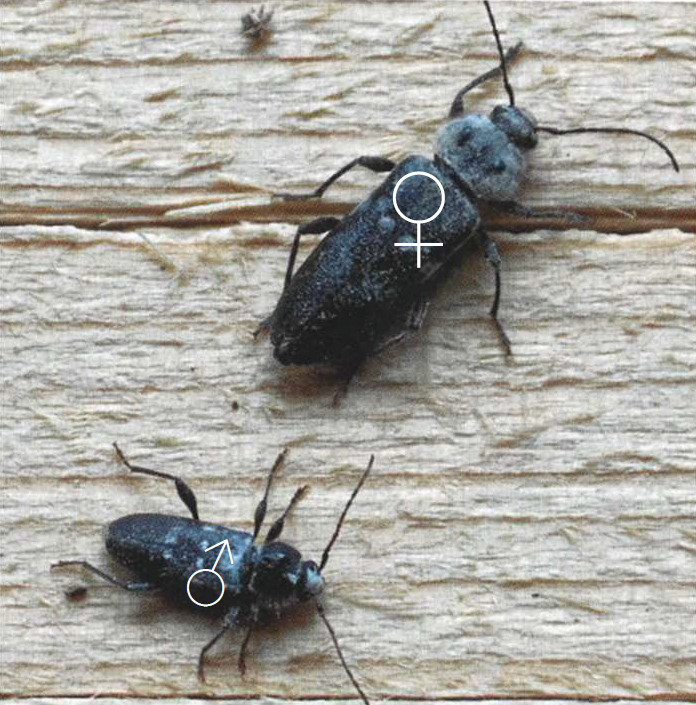
\includegraphics[width=0.9\textwidth]{Grafiken/Beurteilen alter Holzkonstruktionen/Holzschädlinge/Hausbock.png}
    \end{minipage}
        
    \subsection{Gewöhnlicher Nagekäfer: Wissenswertes}
    \begin{minipage}{0.75\textwidth}
        \begin{itemize}
            \item Volksmund: Holzwurm
            \item Verursacht Schäden an Ausstattungsgegenständen
            \item Bauholz ist nicht so sehr betroffen
            \item Er befällt Laub- und Nadelholz und bevorzugt kühlere und feuchte Orte.
                \begin{itemize}
                    \item In Dachstühlen daher seltener anzutreffen
                \end{itemize}
            \item Gelegentliche Befeuchtung befördert die Entwicklung; \\ Trockenheitsperioden verhindern eine solche.
        \end{itemize}
    \end{minipage}
    \begin{minipage}{0.25\textwidth}
        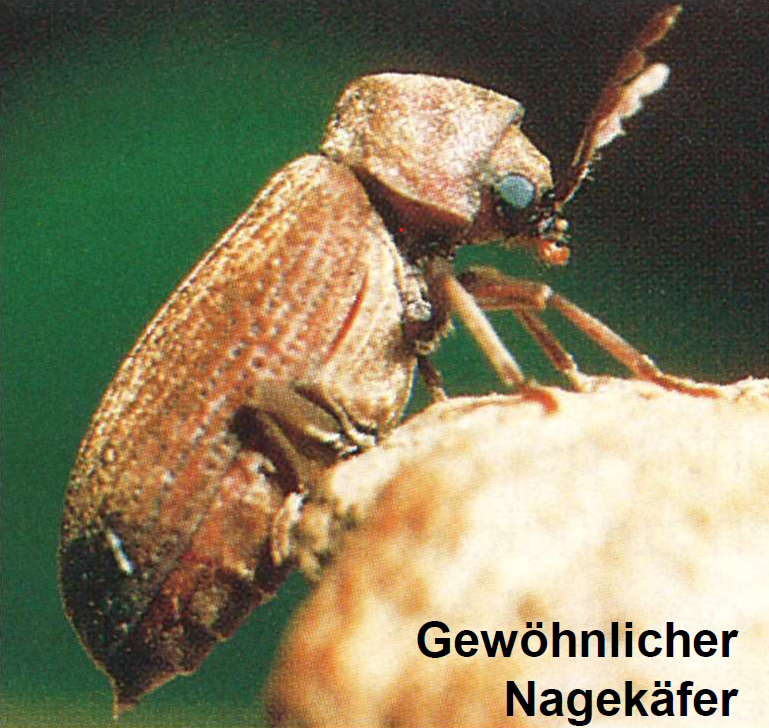
\includegraphics[width=0.9\textwidth]{Grafiken/Beurteilen alter Holzkonstruktionen/Holzschädlinge/Gewoehnlicher Nagekaefer.png}
    \end{minipage}
        
        
    \subsection{Lebensbedingungen – kurz gefasst}
        \begin{itemize}
            \item Bauholzinsektenbefall ab einer Mindestfeuchte von 10\%
                \begin{itemize}
                    \item In regelmäßig beheizten Räumen ist ein Befall unwahrscheinlich (u < 10\%).
                \end{itemize}
            \item Hausbock wärme- und nadelsplintholzliebend
                \begin{itemize}
                    \item Dachgeschoss bzw. -konstruktion
                    \item Befall in altem Holz (>100 a) unwahrscheinlich
                \end{itemize}
            \item Der Gewöhnliche Nagekäfer liebt es kühl und feucht bzw. Nadel- und Laubholz.
                \begin{itemize}
                    \item Kellergeschoss bzw. feuchten Erdgeschoss
                    \item hölzerne Ausstattungsgegenstände
                \end{itemize}
        \end{itemize}
        
    \subsection{Abschließende Hinweise}
        \begin{itemize}
            \item Das künstliche Entziehen der Lebensbedingungen für holzschädigende Organismen kann zur natürlichen Bekämpfung eingesetzt werden.
                \begin{itemize}
                    \item Heißluftanwendung bei Hausbockbefall
                \end{itemize}
            \item Sehr altes Holz wird aufgrund von fehlenden Nährstoffen in der Regel nicht vom Hausbock befallen.
            \item Indizien für einen Befall: sägemehlartige Häufchen, Geräusche
            \item Das damalige Verbauen von frischem Holz begünstigt einen Befall innerhalb der ersten Jahre.
                \begin{itemize}
                    \item Die fortschreitende Trocknung führt dann zu einem Stillstand des Befalls.
                \end{itemize}
        \end{itemize}
        
    

\newpage
\section{Zimmermannsmäßige Holzverbindungen}
    \subsection{Überblick:}
    \begin{minipage}{0.45\textwidth}
        \begin{itemize}
            \item Verbindungsart:
                \begin{itemize}
                    \item Stoß
                    \item Zapfen
                    \item Blatt
                    \item Kamm
                    \item Hals
                    \item Versatz
                    \item Klaue
                    \item Verbindungen des Blockbaus
                    \item Reparaturverbindungen
                \end{itemize}
            \end{itemize}
    \end{minipage}
    \begin{minipage}{0.45\textwidth}
        \begin{itemize}
                \item Verbindungsform:
                \begin{itemize}
                    \item Längsverbindung
                    \item Eckverbindung
                    \item Querverbindung
                    \item Kreuzverbindung
                \end{itemize}
        \end{itemize}
    \end{minipage}
        
    
    
    \subsection{Verbindungsarten:}
    \begin{minipage}{0.45\textwidth}
        \begin{itemize}
                    \item Stumpfer Stoß\\
                        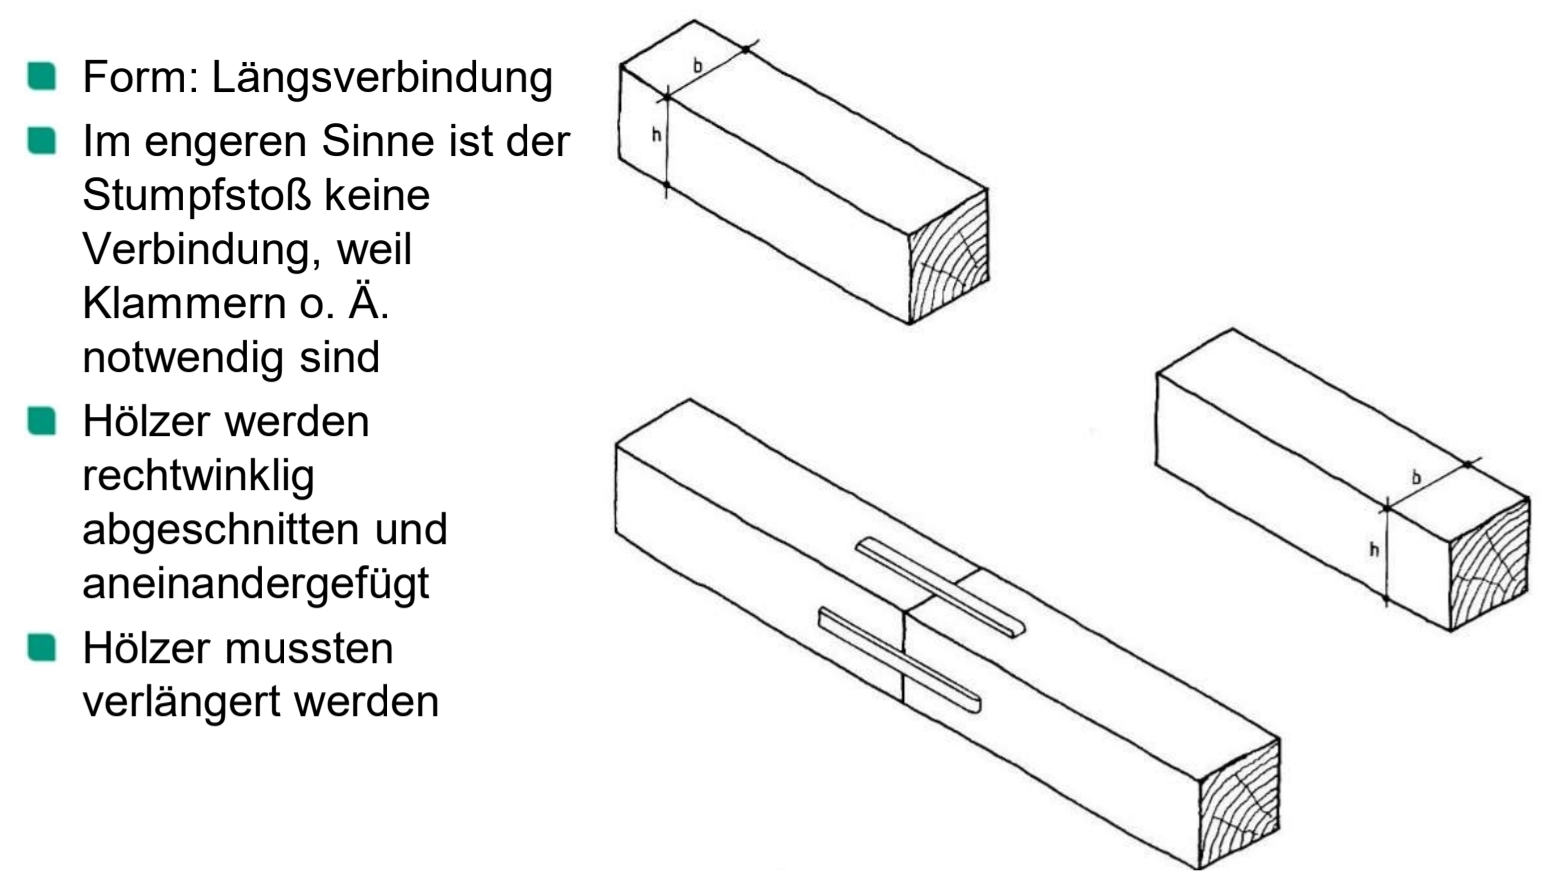
\includegraphics[width=0.9\textwidth]{Grafiken/Zimmermansmaessige Verbindungen/Verbindungsarten/Stumpfer Stoss.jpg}\\
                    \item Gerader Zapfen\\
                        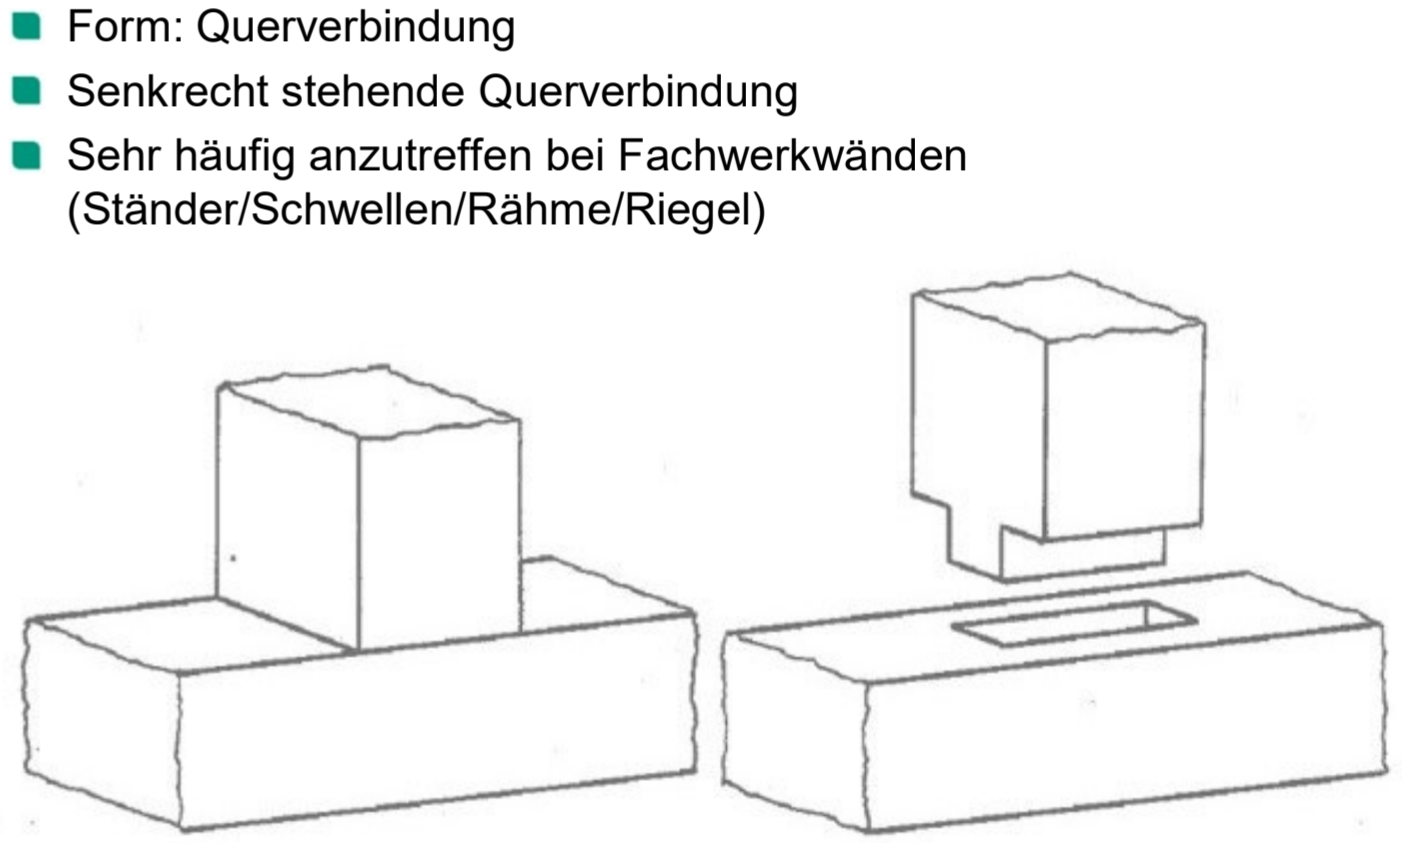
\includegraphics[width=0.9\textwidth]{Grafiken/Zimmermansmaessige Verbindungen/Verbindungsarten/Gerader Zapfen.jpg}\\
                    \item Gerades Blatt\\
                        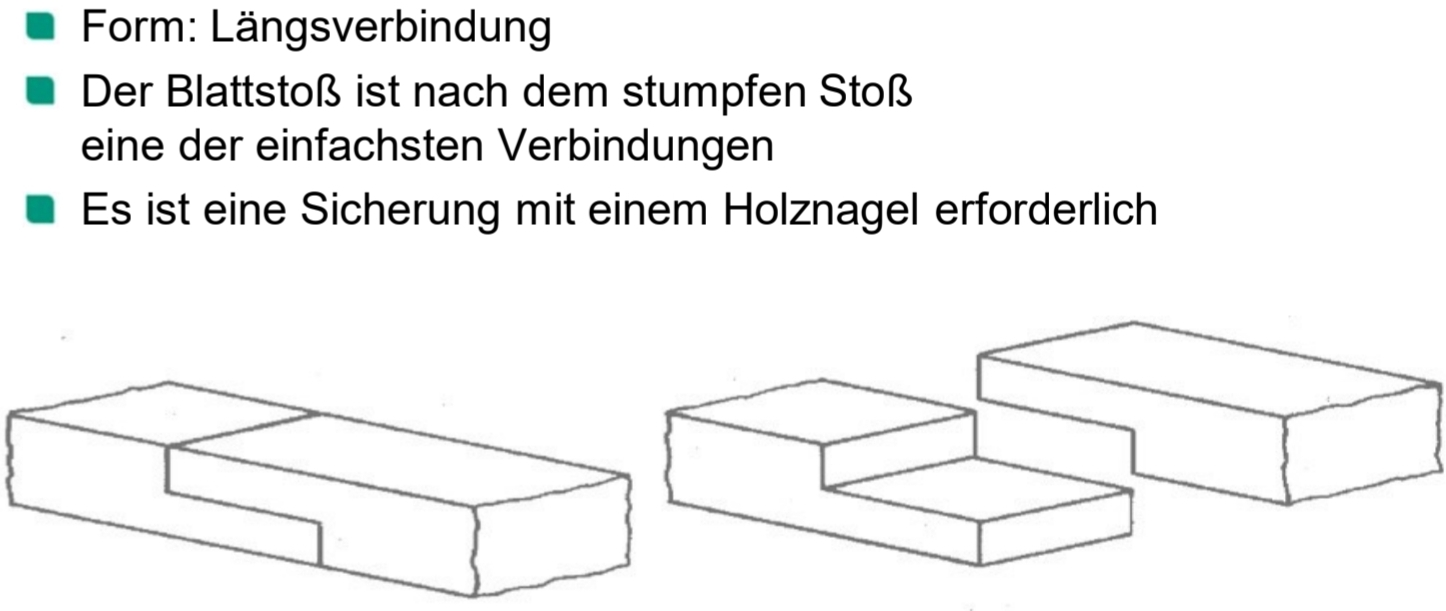
\includegraphics[width=0.9\textwidth]{Grafiken/Zimmermansmaessige Verbindungen/Verbindungsarten/Gerades Blatt.jpg}\\
                    \item Schräges Blatt\\
                        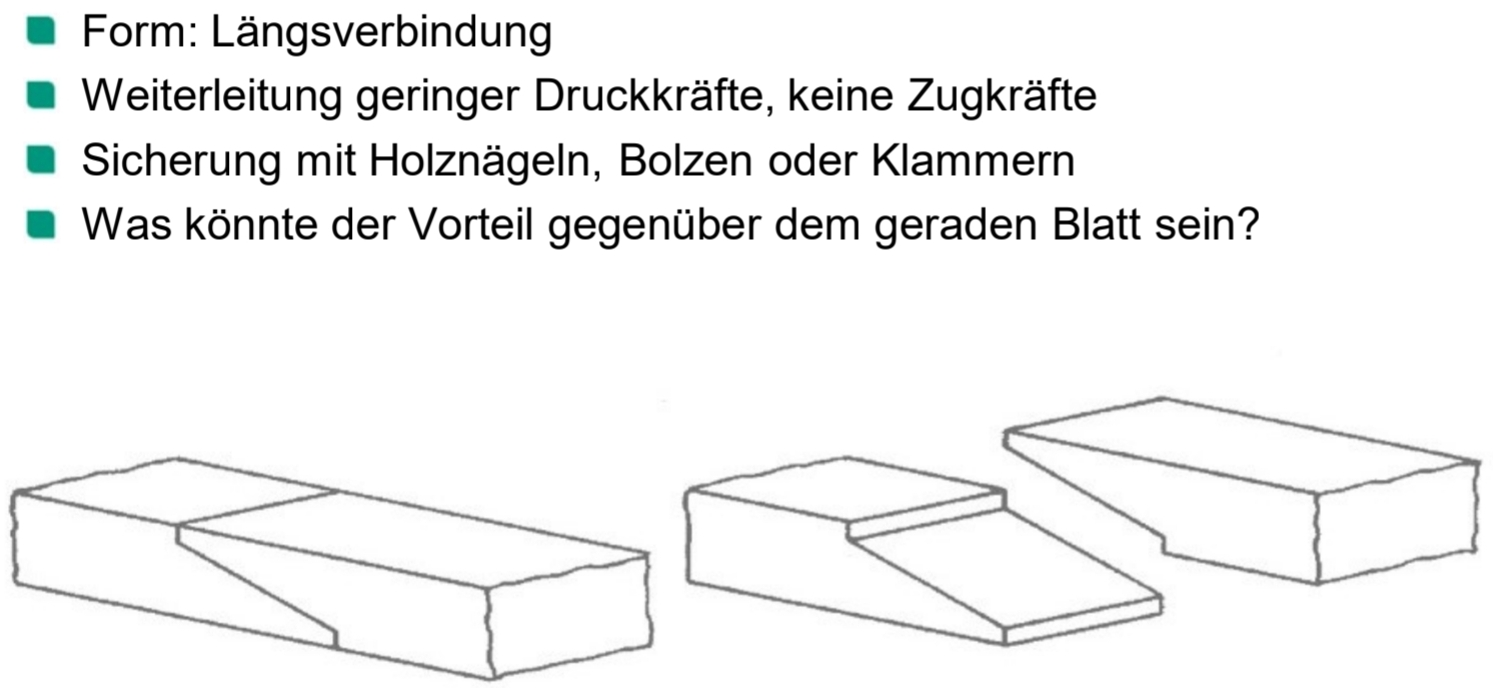
\includegraphics[width=0.9\textwidth]{Grafiken/Zimmermansmaessige Verbindungen/Verbindungsarten/Schraeges Blatt.jpg}\\
        \end{itemize}
    \end{minipage}
    \begin{minipage}{0.45\textwidth}
        \begin{itemize}
                    \item Schräges Blatt mit verdeckten Haken\\
                        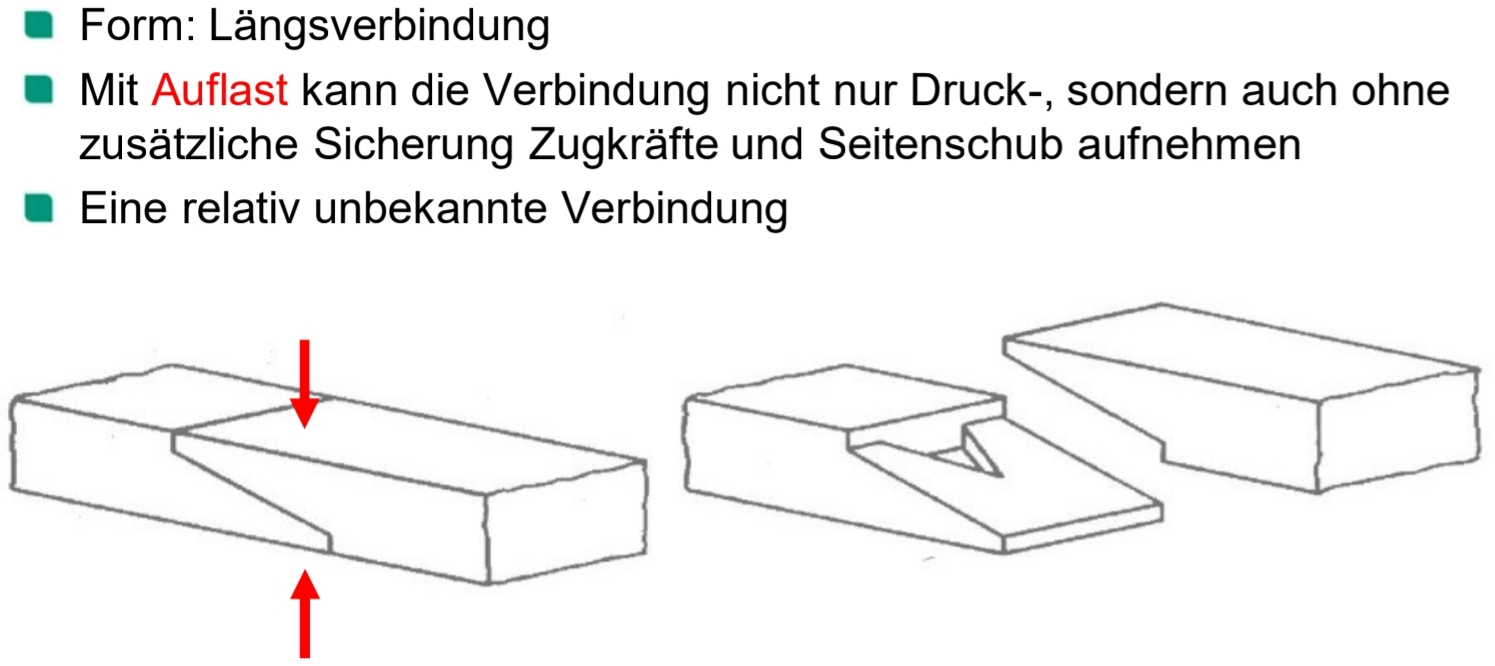
\includegraphics[width=0.9\textwidth]{Grafiken/Zimmermansmaessige Verbindungen/Verbindungsarten/Schraeges Blatt mit verdeckten Haken.jpg}\\
                    \item Gerades Hakenblatt\\
                        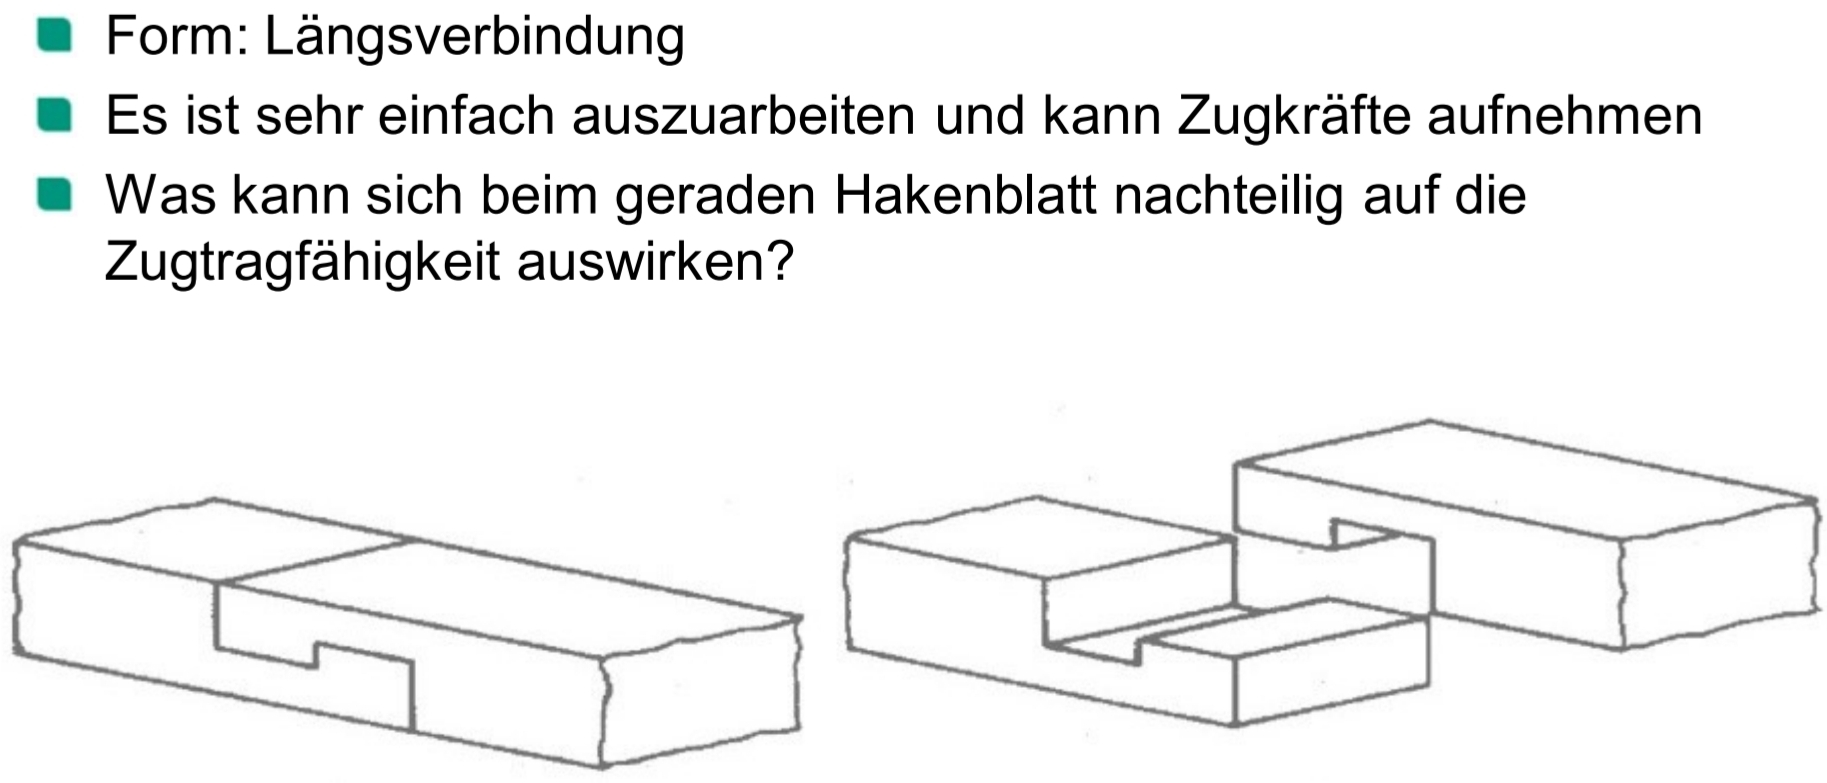
\includegraphics[width=0.9\textwidth]{Grafiken/Zimmermansmaessige Verbindungen/Verbindungsarten/Gerades Hakenblatt.jpg}\\
                    \item Gerades Querblatt\\
                        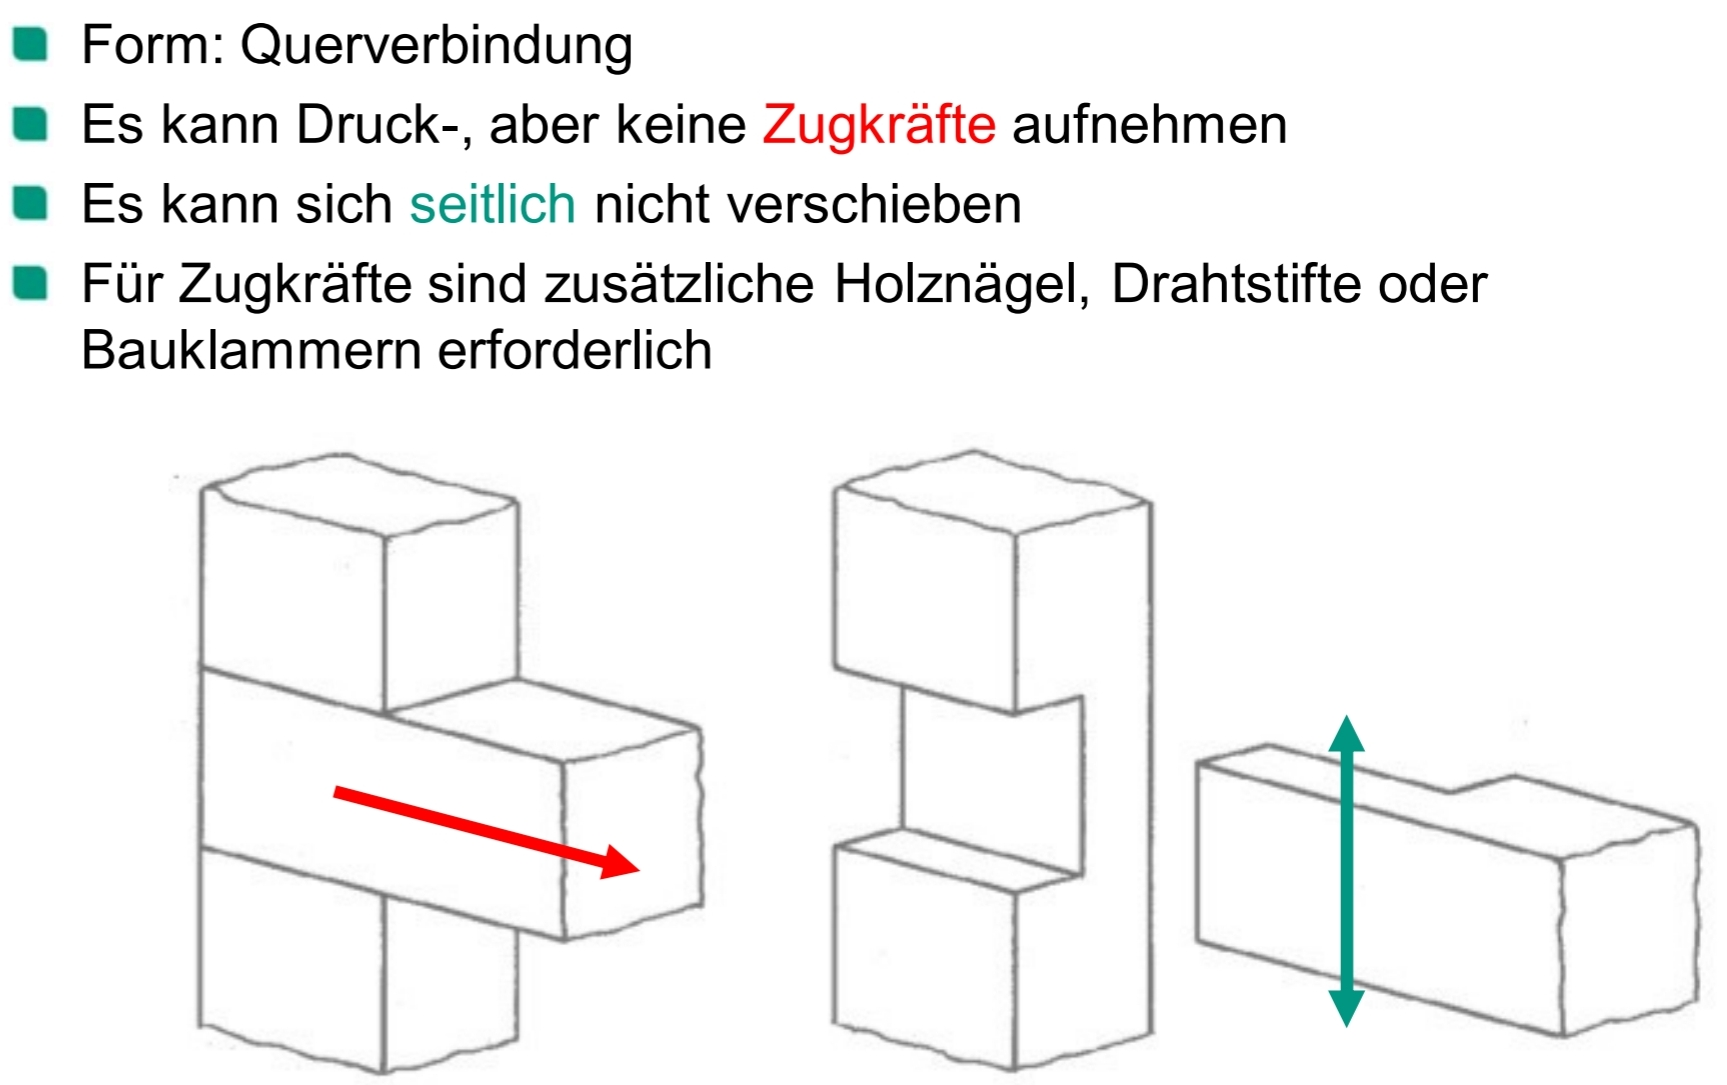
\includegraphics[width=0.9\textwidth]{Grafiken/Zimmermansmaessige Verbindungen/Verbindungsarten/Gerades Querblatt.jpg}\\
                    \item Kreuzblatt\\
                        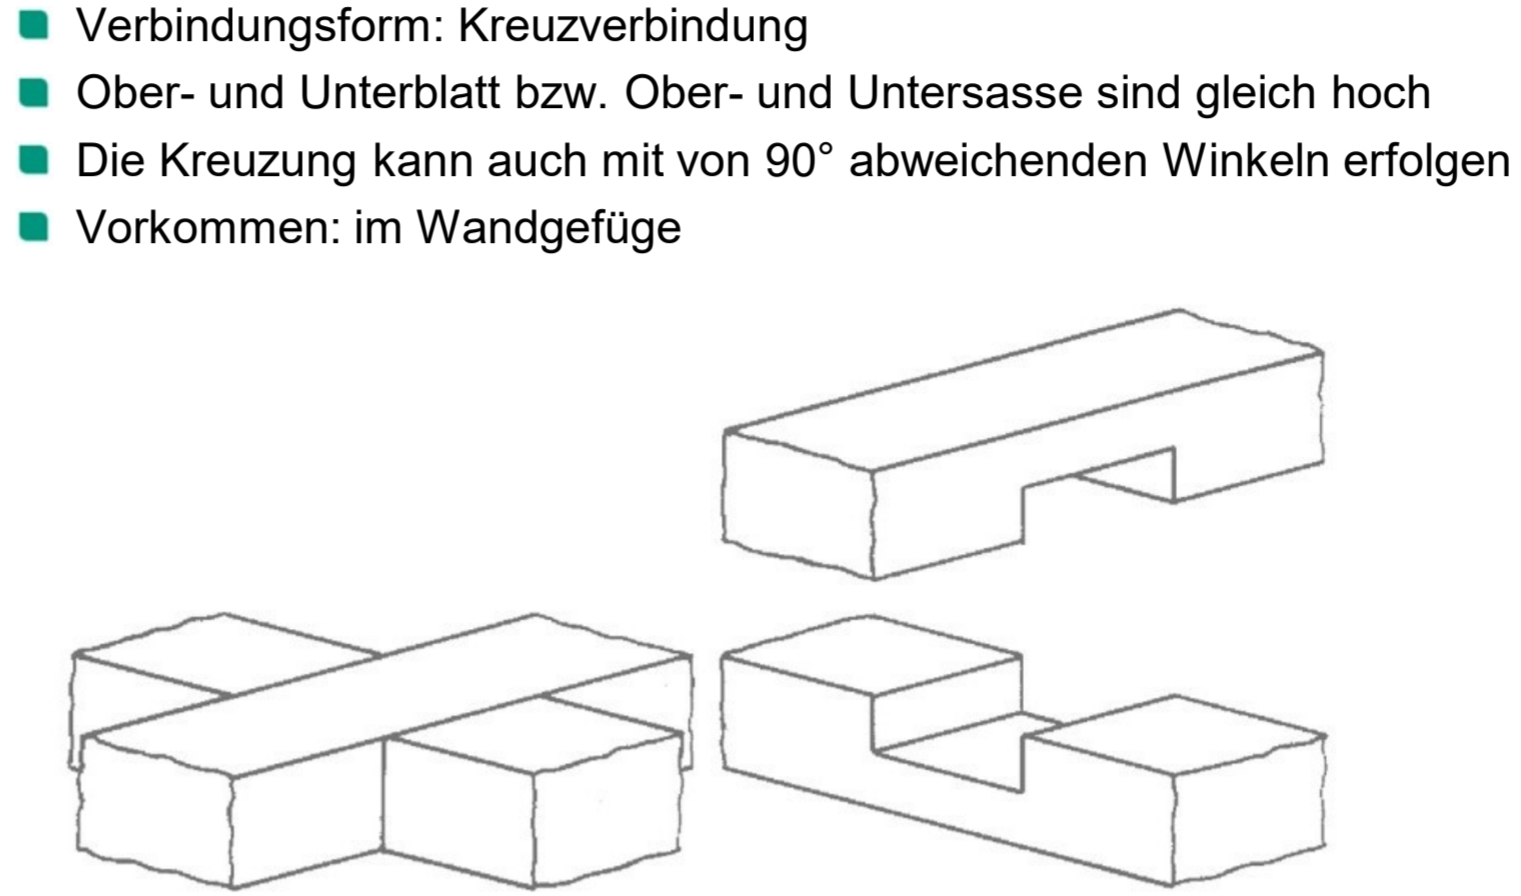
\includegraphics[width=0.9\textwidth]{Grafiken/Zimmermansmaessige Verbindungen/Verbindungsarten/Kreuzblatt.jpg}\\
            \end{itemize}
     \end{minipage}
    
    \begin{minipage}{0.45\textwidth}
        \begin{itemize}
                    \item Einseitiges Schwalbenschwanzblatt\\
                        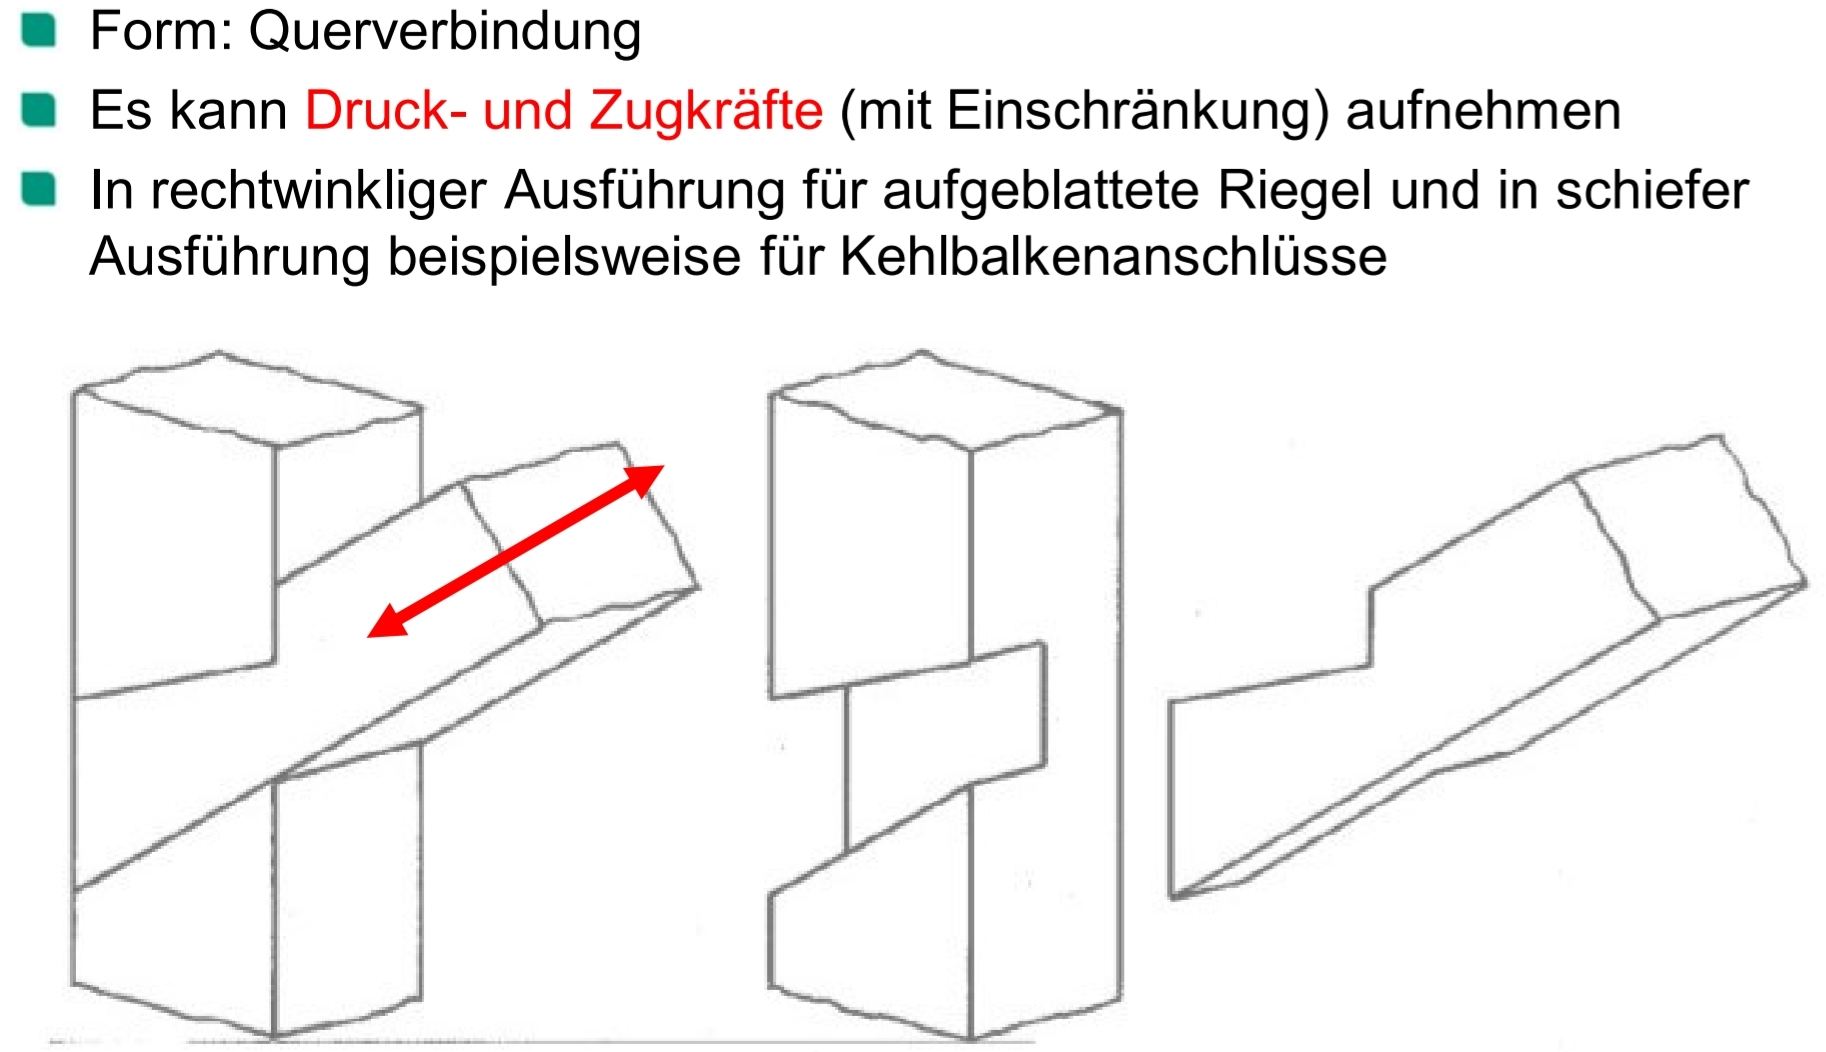
\includegraphics[width=0.9\textwidth]{Grafiken/Zimmermansmaessige Verbindungen/Verbindungsarten/Einseitiges Schwalbenschwanzblatt.jpg}\\
                    \item Zweiseitig abgesetztes Kreuzblatt\\
                        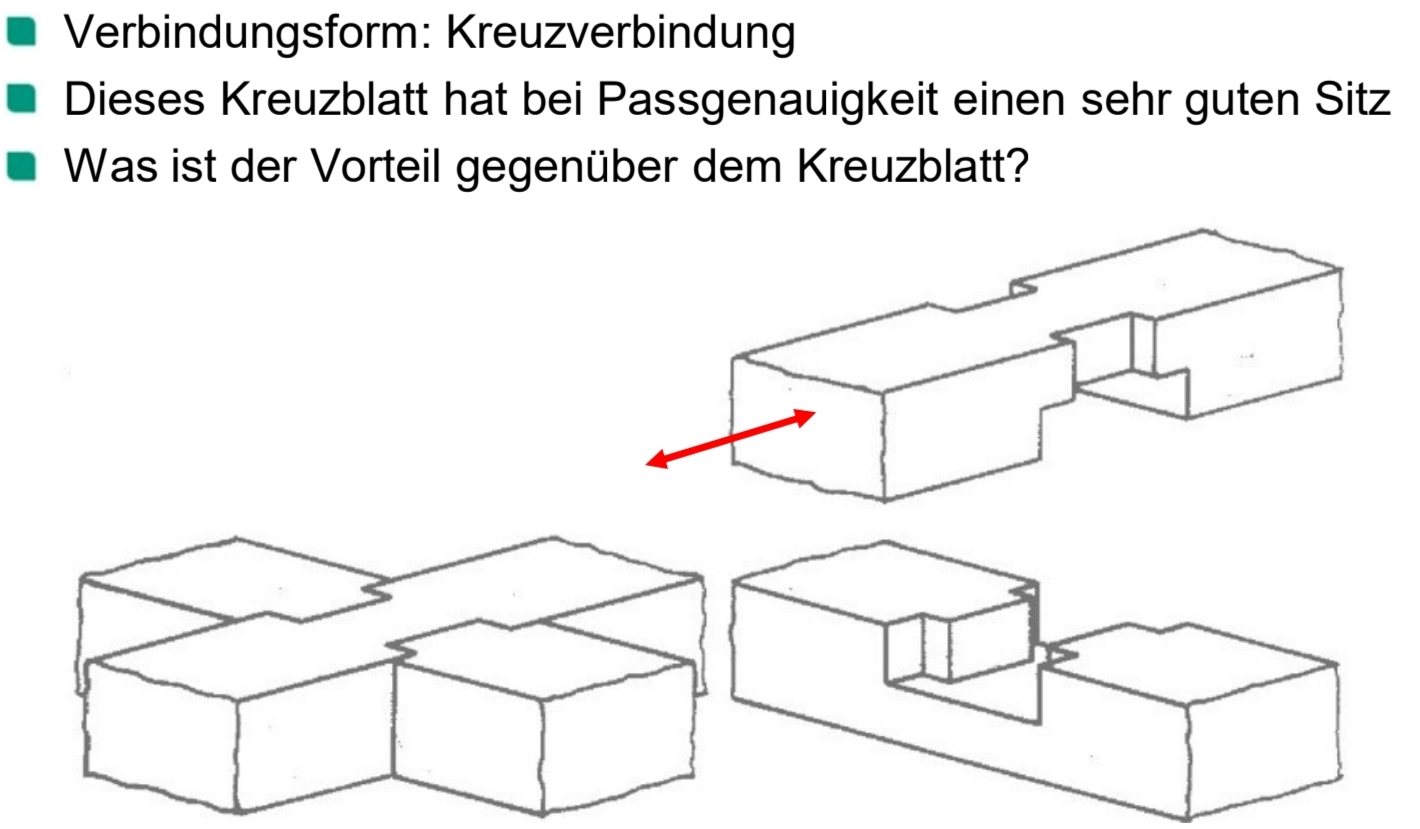
\includegraphics[width=0.9\textwidth]{Grafiken/Zimmermansmaessige Verbindungen/Verbindungsarten/Zweiseitig abgesetztes Kreuzblatt.jpg}\\
                    \item Einfacher bündiger Blattzapfen\\
                        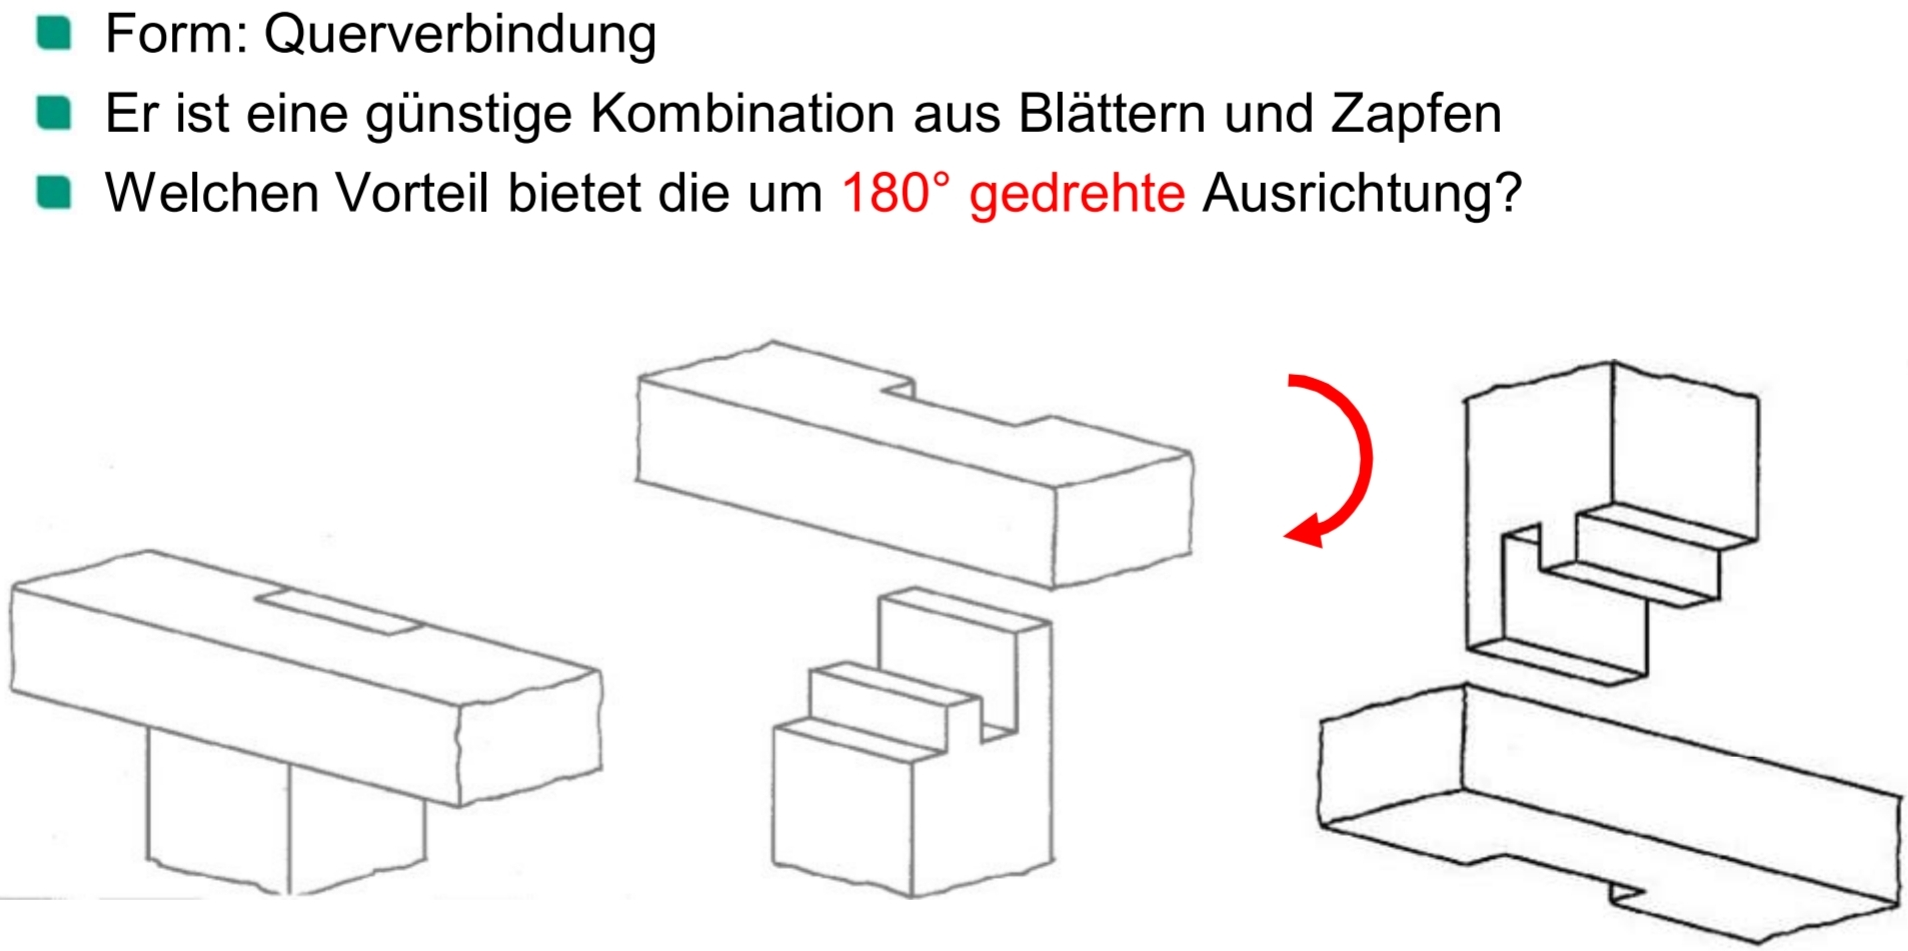
\includegraphics[width=0.9\textwidth]{Grafiken/Zimmermansmaessige Verbindungen/Verbindungsarten/Einfacher buendiger Blattzapfen.jpg}\\
                    \item Doppelkamm\\
                        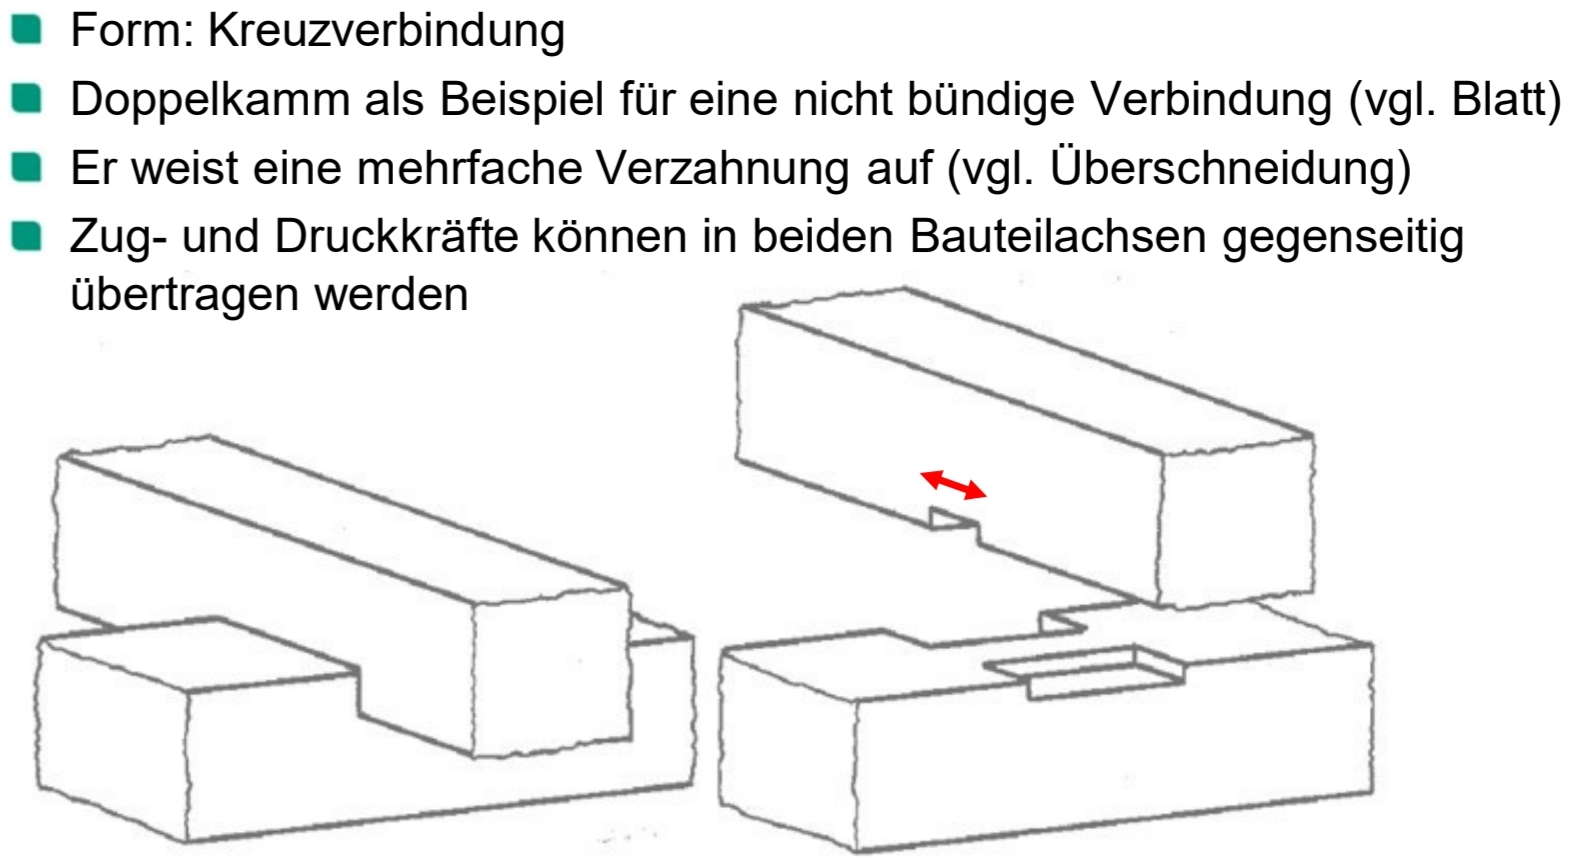
\includegraphics[width=0.9\textwidth]{Grafiken/Zimmermansmaessige Verbindungen/Verbindungsarten/Doppelkamm.jpg}\\
                    \item Stirnversatz\\
                        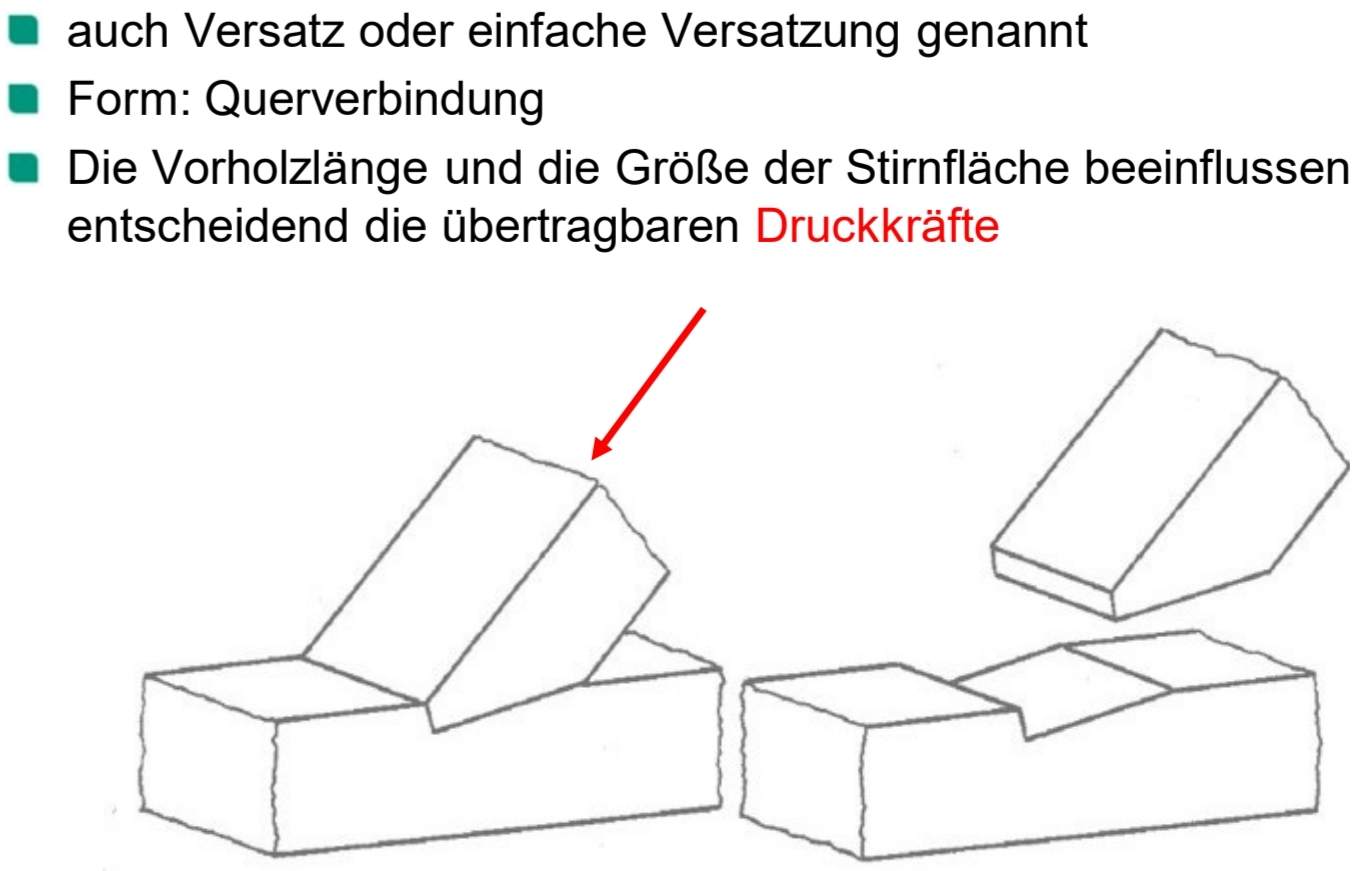
\includegraphics[width=0.9\textwidth]{Grafiken/Zimmermansmaessige Verbindungen/Verbindungsarten/Stirnversatz.jpg}\\
        \end{itemize}
    \end{minipage}
    \begin{minipage}{0.45\textwidth}
        \begin{itemize}
                    \item Aufklauung durch Hirnschnitt Sparren\\
                        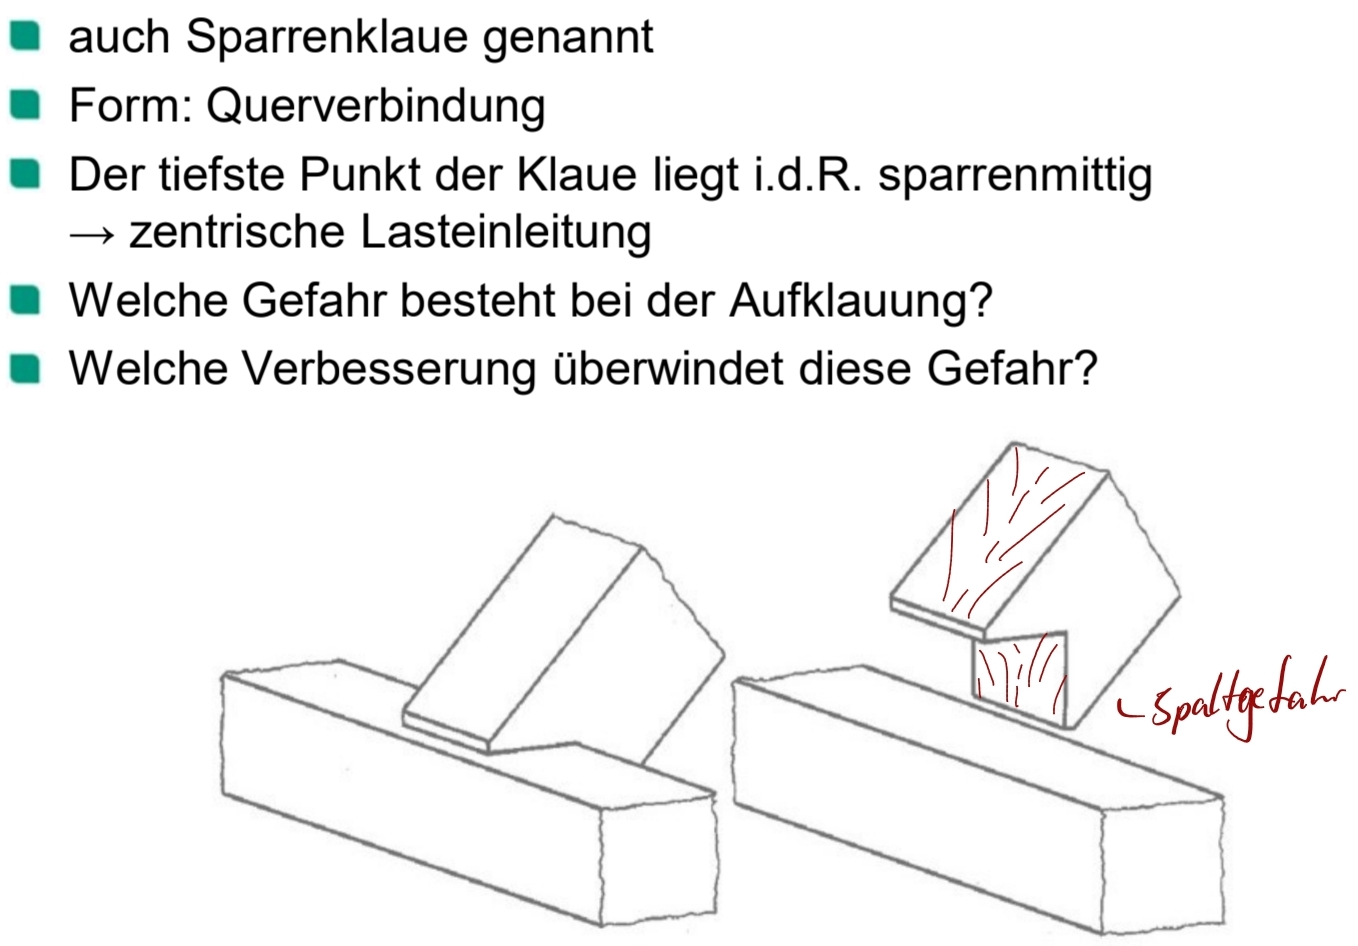
\includegraphics[width=0.9\textwidth]{Grafiken/Zimmermansmaessige Verbindungen/Verbindungsarten/Aufklauung durch Hirnschnitt Sparren.jpg}\\
                    \item Aufklauung mit Anschnitt Pfette\\
                        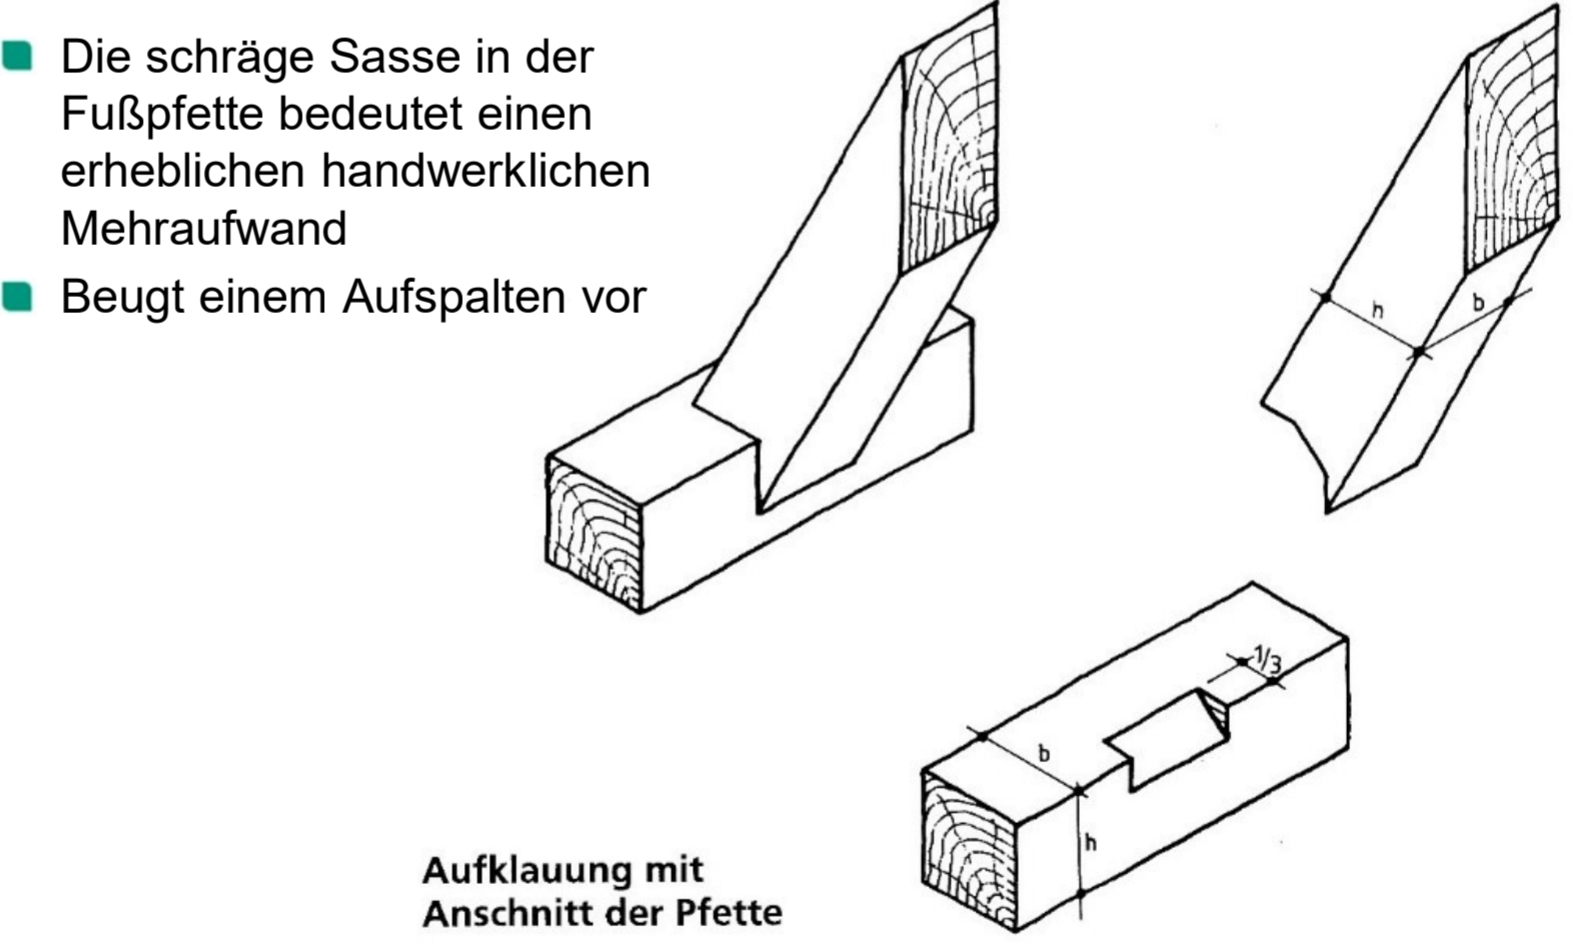
\includegraphics[width=0.9\textwidth]{Grafiken/Zimmermansmaessige Verbindungen/Verbindungsarten/Aufklauung mit Anschnitt Pfette.jpg}\\
                    \item Zimmermansmääige Holzverbindungen\\
                        \includegraphics[width=0.9\textwidth]{Grafiken/Zimmermansmaessige Verbindungen/Verbindungsarten/Zimmermansmaessige Holzverbindungen.jpg}\\
                    \item Historische Metallverbindungen Holzbau\\
                        \includegraphics[width=0.9\textwidth]{Grafiken/Zimmermansmaessige Verbindungen/Verbindungsarten/Historische Metallverbindungen Holzbau.jpg}\\
        \end{itemize}
     \end{minipage}

\subsection{Exkurs zu Stirnversätzen:}
    Formeln Scherspannung:
    \begin{itemize}
        \item Scherrspannung $\tau_{m,d}$ im Vorholz: $\tau_{m,d} = \frac{F_d \cdot \cos \alpha}{b_{eff}\cdot l_v}$
        \item $l_{v,max,ansetzbar} = 8 \cdot t_v$
        \item $\tau_{m,d} < f_{v,d}$
    \end{itemize}

    Geometrien und Kräfte:
    \vspace*{3mm}\\
    \includegraphics[width=0.4\textwidth]{Grafiken/Zimmermansmaessige Verbindungen/Stirnversatz/Stirnversatz Ueberblick.png}
    \includegraphics[width=0.4\textwidth]{Grafiken/Zimmermansmaessige Verbindungen/Stirnversatz/Stirnversatz Einfluss Vorholzlaenge.png}
    \includegraphics[width=0.2\textwidth]{Grafiken/Zimmermansmaessige Verbindungen/Stirnversatz/Stirnversatz Kraefte.png}

     Auswertung:
     \begin{itemize}
         \item Scherspannungen:
            \begin{itemize}
                \item Falls in der Scherebene nach eingehender Untersuchung keine Schwindrisse vorhanden sind, darf die Scherspannung mit $k_{\mathrm{cr}}=1$ berechnet werden.
                \item Das heißt: Die charakteristische Schubfestigkeit $f_{\mathrm{v}, \mathrm{k}}=4,0 \mathrm{~N} / \mathrm{mm}^2$ wird in der gesamten Scherebene als wirksam angenommen.
            \end{itemize}
        \item Druckspannungen:
            \begin{itemize}
                \item Falls im maßgebenden Stirnbereich nur kleine Äste (S13) vorhanden sind, kann in diesem Bereich die Druckfestigkeit für $\mathrm{C} 30$ verwendet werden.
                \item Falls zugleich eine Rohdichte von über $450 \mathrm{~kg} / \mathrm{m} 3$ vorhanden* ist, kann die Druckfestigkeit für $\mathrm{C} 40$ verwendet werden.
                \item *Hierzu sind Ihnen Untersuchungsmethoden bekannt.
            \end{itemize}
     \end{itemize}

\newpage
\section{Denkmalpflegerische Arbeit:}
    \begin{itemize}
        \item Beschäftigt sich mit Reparaturen und Konstruktionen für historische Tragstrukturen
        \item Einleitungstext:\\
            Nachdem ein Bauwerk als Baudenkmal identifiziert wurde, ist es durch das individuelle Zusammenspiel von
                \begin{itemize}
                    \item Funktion und Gebrauchswert,
                    \item Form und Erscheinungsbild,
                    \item Material oder Baustoff sowie
                    \item Bautechnik und Baugefüge
                \end{itemize}
            gekennzeichnet und ab diesem Zeitpunkt einem Wandel unterworfen. An dieser Stelle setzen die denkmalpflegerischen Konzepte an, die unterschiedliche Sichtweisen auf und unterschiedliche Formen der Auseinandersetzung mit diesem Wandel reflektieren. Wir kennen heute sechs unterschiedliche denkmalpflegerische Konzepte.
        \item Auftrag und Aufgaben des Bauingenieurs:\\
            \begin{tabular}{c|c|c|c|}
            \cline{2-4}
             &
              Sockelkriterien &
              1. Zusatzkriterium &
              2. Zusatzkriterium \\ \hline
            \multicolumn{1}{|c|}{Instandsetzung von Baudenkmälern} &
              \multirow{3}{*}{\begin{tabular}[c]{@{}c@{}}Gestalt\\ Funktion\\ Konstruktion\\ Kosten\end{tabular}} &
              \multirow{2}{*}{\begin{tabular}[c]{@{}c@{}}Technische\\ Wirksamkeit\end{tabular}} &
              \begin{tabular}[c]{@{}c@{}}historische\\ Bedeutung\end{tabular} \\ \cline{1-1} \cline{4-4} 
            \multicolumn{1}{|c|}{\begin{tabular}[c]{@{}c@{}}Allgemeine\\ Instandsetzung\\ und Erneuerung\\ von Altbauten\end{tabular}} &
               &
               &
              - \\ \cline{1-1} \cline{3-4} 
            \multicolumn{1}{|c|}{Neubau} &
               &
              - &
              - \\ \hline
            \end{tabular}
       \end{itemize}
\subsection{Unterscheidung additiv und reine Reparaturen}
       \begin{itemize}
        \item Unterscheidung zwischen reinen Reparaturen und solchen mit additiven Teilen bei lokalen Eingriffen
        \item Unterscheidung zwischen additiven und substituierenden Konstruktionen bei technischen Sicherungsmaßnahmen
            \begin{itemize}
                \item Reine Reparatur: 
                    \begin{itemize}
                        \item Keine Veränderung des statischen Prinzips und der formalen Ausbildung
                        \item Erneuerung oder Teilerneuerung von schadhaften Teilen in gleicher Anordnung, Dimensionierung und Form
                        \item Orientierung an historischen Gegebenheiten
                        \item Anpassung neuer Teile an die historische Substanz
                    \end{itemize}
                \item Reparatur mit additiven Teilen: 
                    \begin{itemize}
                        \item Hinzufügen von Bauteilen, die im historischen Gefüge nicht existierten
                        \item keine oder geringe Verluste an der Substanz
                        \item Befunde bleiben erhalten, Möglichkeit zur Entfernung ohne große Spuren
                        \item Wirkung auf das historische Gesamtbild muss bedacht werden
                    \end{itemize}
                \item Substituierende Konstruktion: 
                    \begin{itemize}
                        \item Entlastung der gesamten Altkonstruktion
                        \item vollständige Entlastung oder wesentliche statische Tragwirkungen der alten Struktur
                        \item substituierenden Konstruktion von Entlastung bis hin zur Stützung der alten Struktur
                    \end{itemize}
            \end{itemize}
        \item Beispiel additive Maßnahmen:\\
            \includegraphics[width=0.45\textwidth]{Grafiken/Denkmalpflegerische Arbeit/Additive Massnahmen/Aufhaengung Decke und Ersatz Lager Vorholz 1.png}
            \includegraphics[width=0.45\textwidth]{Grafiken/Denkmalpflegerische Arbeit/Additive Massnahmen/Additive Massnahmen - Zugkraefte Stuhlsaeule aufnehmen.png}\\
            \includegraphics[width=0.45\textwidth]{Grafiken/Denkmalpflegerische Arbeit/Additive Massnahmen/Aufhaengung Decke und Ersatz Lager Vorholz 2.png}
            \includegraphics[width=0.45\textwidth]{Grafiken/Denkmalpflegerische Arbeit/Additive Massnahmen/Verbund durch Laschen.png} 
    \end{itemize}

    \subsection{Denkmalsch(m)utz - Pflegekonzepte}
    \begin{itemize}
        \item Altern-Lassen
            \begin{itemize}
                \item ursprüngliche Funktion eines Bauwerks und diejenige seiner Teile gehen allmählich verloren
                \item Gebrauchswert zunächst eingeschränkt, um schließlich vollständig verloren zu gehen
                \item Form verfällt
                \item Erscheinungsbild verschlechtert sich
                \item Material oder Baustoffe zersetzen sich, (im Falle von Holz) verfaulen oder zerfallen
                \item bautechnische Zusammenhalt zerbricht
            \end{itemize}
        \item Pflegen
            \begin{itemize}
                \item Altern akzeptiert
                \item Maßnahmen um Prozess des Alterns zu verlangsamen
                \item Funktion der fortwährend nachlassenden Leistungsfähigkeit des Bauwerks angepasst oder von zusätzlichen Hilfskonstruktionen ganz oder teilweise übernommen
                \item Gebrauchswert nimmt ab
                \item Alters- und Gebrauchsspuren sichtbar
                \item permanente Hilfskonstruktionen
                \item Ist-Zustand des Materials oder Baustoffs wird nicht manipuliert
                \item durch Verschleißschichten geschützt
                \item Schwachstellen akzeptiert oder durch Hilfskonstruktionen ganz oder teilweise entlastet
            \end{itemize}
        \item Konservieren
            \begin{itemize}
                \item Altern und den Verfallsprozess – zumindest theoretisch – zum Stillstand zu bringen
                \item Bauwerk den weiteren bzw. zukünftigen Einwirkungen entzogen oder dagegen abgeschirmt wird
                \item verändert Funktion, die Bauwerk nun nicht mehr aktiv erfüllt
                \item Gebrauchswert kann sich völlig verändern
                \item Schutzschichten oder Konservierungsmittel verändern Erscheinungsbild des gesamten Umfelds durch das Konservieren
                \item konserviertes Material kann nicht mehr als das ursprüngliche Material anerkannt werden
            \end{itemize}
        \item Reparieren
            \begin{itemize}
                \item historische Werdegang eines Bauwerks respektiert
                \item Funktionsverluste werden identifiziert und in der Regel behutsam ausgeglichen
                \item Gebrauchswert bleibt auf höheren und ursprünglicheren Niveau erhalten
                \item verändern in der Regel die Form in lokal begrenzen Bereichen
                \item Erscheinungsbild nicht mehr als erforderlich beeinträchtigt (Denkmalschutz)
                \item geschädigter Substanz durch in Frage kommende alternative Materialien oder Baustoffe ersetzt
            \end{itemize}
        \item Erneuern
            \begin{itemize}
                \item neue Anforderung an das Bauwerk
                \item bisherige Gebrauchswert und neuer Anforderungen zumindest in Teilen nicht mehr deckungsgleich
                \item Erscheinungsbild durch neu hinzugekommene Elemente geprägt
                \item Materialschäden werden nicht akzeptiert
                \item umfangreicheren Überarbeitung oder mit einem Austausch von Bauteilen
            \end{itemize}
        \item Rekonstruieren
            \begin{itemize}
                \item früherer bereits nicht mehr existenter Zustand wiederhergestellt
                \item rein technisch betrachtet ein Neubau
                \item bisherige Funktion findet ein Ende und es wird diejenige reaktiviert, die der Rekonstruktion entspricht
                \item Material sollte nicht im Widerspruch stehen zum Material der tatsächlichen historischen Vorbilder
                \item Auf vergangene Bautechnik und das vergangene Baugefüge wird zurückgegriffen
            \end{itemize}
    \end{itemize}
    \subsection{Überblick über Sanierungskonzepte:}
    \resizebox{\textwidth}{!}{\begin{tabular}{l|l|l|l|}
            \cline{2-4}
             &
              \begin{tabular}[c]{@{}l@{}}1. Konzept\\ Altern-Lassen\end{tabular} &
              \begin{tabular}[c]{@{}l@{}}2. Konzept\\ Pflegen\end{tabular} &
              \begin{tabular}[c]{@{}l@{}}3. Konzept\\ Konservieren\end{tabular} \\ \hline
            \multicolumn{1}{|l|}{\begin{tabular}[c]{@{}l@{}}Funktion\\ bzw.\\ Gebrauchswert\end{tabular}} &
              \begin{tabular}[c]{@{}l@{}}Funktion und Gebrauchswert\\ gehen verloren\end{tabular} &
              \begin{tabular}[c]{@{}l@{}}Funktion wird angepasst;\\ Gebrauchswert sinkt\end{tabular} &
              \begin{tabular}[c]{@{}l@{}}Funktion geht verloren;\\ Gebrauchswert verändert\\ sich\end{tabular} \\ \hline
            \multicolumn{1}{|l|}{\begin{tabular}[c]{@{}l@{}}Form\\ bzw.\\ Erscheinungsbild\end{tabular}} &
              \begin{tabular}[c]{@{}l@{}}Form und Erscheinungsbild\\ verschwinden\end{tabular} &
              \begin{tabular}[c]{@{}l@{}}Form und Erscheinungsbild\\ verändern sich\end{tabular} &
              \begin{tabular}[c]{@{}l@{}}Funktion und Erscheinungsbild\\ bleiben erhalten, nicht\\ aber hinsichtlich des Umfelds\end{tabular} \\ \hline
            \multicolumn{1}{|l|}{\begin{tabular}[c]{@{}l@{}}Material\\ oder\\ Baustoff\end{tabular}} &
              \begin{tabular}[c]{@{}l@{}}Material oder Baustoff\\ zerfallen\\ (z.B. Holz verfault)\end{tabular} &
              \begin{tabular}[c]{@{}l@{}}Material oder Baustoff\\ werden erhalten\end{tabular} &
              \begin{tabular}[c]{@{}l@{}}Material u. Baustoff bleiben\\ erhalten oder werden\\ durch Konservierung\\ verändert\end{tabular} \\ \hline
            \multicolumn{1}{|l|}{\begin{tabular}[c]{@{}l@{}}Bautechnik\\ bzw.\\ Baugefüge\end{tabular}} &
              \begin{tabular}[c]{@{}l@{}}Bautechnik geht verloren;\\ Baugefüge zerfällt\end{tabular} &
              \begin{tabular}[c]{@{}l@{}}Bautechnik und Baugefüge\\ bleiben erhalten\end{tabular} &
              \begin{tabular}[c]{@{}l@{}}Bautechnik und Baugefüge\\ verlieren oft ihre Bestimmung\end{tabular} \\ \hline
    \end{tabular}}
    \vspace*{3mm}
    \resizebox{\textwidth}{!}{\begin{tabular}{l|l|l|l|}
            \cline{2-4}
             &
              \begin{tabular}[c]{@{}l@{}}4. Konzept\\ Reparieren\end{tabular} &
              \begin{tabular}[c]{@{}l@{}}5. Konzept\\ Erneuern\end{tabular} &
              \begin{tabular}[c]{@{}l@{}}6. Konzept\\ Rekonstruieren\end{tabular} \\ \hline
            \multicolumn{1}{|l|}{\begin{tabular}[c]{@{}l@{}}Funktion\\ bzw.\\ Gebrauchswert\end{tabular}} &
              \begin{tabular}[c]{@{}l@{}}Funktion wird wiederhergestellt;\\ Gebrauchswert bleibt\\ erhalten\end{tabular} &
              \begin{tabular}[c]{@{}l@{}}Funktion wird erweitert;\\ Gebrauchswert verändert\\ sich (steigt ggf.)\end{tabular} &
              \begin{tabular}[c]{@{}l@{}}Die bisherige Funktion\\ weicht einer früheren\end{tabular} \\ \hline
            \multicolumn{1}{|l|}{\begin{tabular}[c]{@{}l@{}}Form\\ bzw.\\ Erscheinungsbild\end{tabular}} &
              \begin{tabular}[c]{@{}l@{}}Form und Erscheinungsbild\\ werden lokal der Maßnahme\\ entsprechend verändert\end{tabular} &
              \begin{tabular}[c]{@{}l@{}}Form und Erscheinungsbild\\ werden verändert\\ bzw. erneuert\end{tabular} &
              \begin{tabular}[c]{@{}l@{}}Rückkehr zu einer früheren\\ Form bzw. zu einem früheren\\ Erscheinungsbild\end{tabular} \\ \hline
            \multicolumn{1}{|l|}{\begin{tabular}[c]{@{}l@{}}Material\\ oder\\ Baustoff\end{tabular}} &
              \begin{tabular}[c]{@{}l@{}}Material oder Baustoff\\ werden lokal ersetzt\end{tabular} &
              \begin{tabular}[c]{@{}l@{}}Material oder Baustoff\\ werden im Bauteilmaßstab\\ ersetzt\end{tabular} &
              \begin{tabular}[c]{@{}l@{}}Material oder Baustoff\\ sind neu, aber getreu historischem\\ Vorbild\end{tabular} \\ \hline
            \multicolumn{1}{|l|}{\begin{tabular}[c]{@{}l@{}}Bautechnik\\ bzw.\\ Baugefüge\end{tabular}} &
              \begin{tabular}[c]{@{}l@{}}Bautechnik und Baugefüge\\ bleiben weitgehend\\ erhalten\end{tabular} &
              \begin{tabular}[c]{@{}l@{}}Neue Bautechnik kommt\\ hinzu; ggf. weiteres neues\\ Baugefüge\end{tabular} &
              \begin{tabular}[c]{@{}l@{}}Bautechnik und Baugefüge\\ getreu historischem\\ Vorbild\end{tabular} \\ \hline
    \end{tabular}}

\subsection{Materialeigenschaften:}
    \resizebox{\textwidth}{!}{\begin{tabular}{l|l|l|}
            \cline{2-3}
             &
              \begin{tabular}[c]{@{}l@{}}Vorteile\end{tabular} &
              \begin{tabular}[c]{@{}l@{}}Nachteile\end{tabular} \\ \hline
            \multicolumn{1}{|l|}{\begin{tabular}[c]{@{}l@{}}Holz\end{tabular}} &
              \begin{tabular}[c]{@{}l@{}}i.d.R. lokal/regional verfügbar\\
                                        große Vielfalt unterschiedlicher Holzarten\\
                                        relativ hohe Druckfestigkeit in Faserrichtung\\
                                        relativ hoher $\mathrm{E}-\mathrm{Modul}$ in Faserrichtung\\
                                        leichte handwerkliche/industrielle Bearbeitung\\
                                        Holz ist eine Art Urbaustoff, der den Menschen\\
                                        seit jeher umgibt und begleitet\end{tabular} &
              \begin{tabular}[c]{@{}l@{}}zunächst \enquote{unsortierter} Naturbaustoff\\
                                        sehr niedrige Querzugfestigkeit\\
                                        niedriger E-Modul quer zur Faserrichtung\\
                                        je nach Holzart eingeschränkte Dauerhaftigkeit\\
                                        brennbar (beachte kohlebefeuerte Lokomotiven)\\
                                        limitierte Bauteillängen bei Schnittholz\\
                                        hygroskopisch\\
                                        (Einfluss auf E-Modul, Festigkeit und Formtreue)\\
                                        eingeschränkte Leistungsfähigkeit bei\\
                                        zugbeanspruchten (Längs-)Verbindungen\end{tabular} \\ \hline
            \multicolumn{1}{|l|}{\begin{tabular}[c]{@{}l@{}}Gusseisen\end{tabular}} &
              \begin{tabular}[c]{@{}l@{}}homogen und isotrop\\
                                        sehr geeignet für Formvielfalt\\
                                        hohe Druckfestigkeit\\
                                        hoher E-Modul\end{tabular} &
              \begin{tabular}[c]{@{}l@{}}wirtschaftlich erst bei großen Stückzahlen\\ je nach Legierung spröde\end{tabular} \\ \hline
            \multicolumn{1}{|l|}{\begin{tabular}[c]{@{}l@{}}Schmiedeeisen\end{tabular}} &
              \begin{tabular}[c]{@{}l@{}}weitgehend homogen bzw. isotrop\\
                                        höhere Zugfestigkeit im Vergleich mit Holz\\
                                        höherer E-Modul im Vergleich mit Holz\\
                                        guter Baustoff für große Spannweiten\\
                                        gutes Material für Verbindungsmittel o.Ä.\\
                                        des Holzbaus\\
                                        gutes Material in Kombination mit Holz\end{tabular} &
              \begin{tabular}[c]{@{}l@{}}zentrale Herstellung in Eisenhütten\\
                                        stabilitätsgefährdet (Knicken, Beulen)\\
                                        aufwändige Bearbeitung\\
                                        Korrosion\\
                                        starke Festigkeitseinbußen bei Brand\\
                                        Ermüdungsgefahr bei Kerbfällen und \\
                                        nicht vorwiegend ruhender Belastung\\ 
                                        (beachte Brückenbau)\\
                                        Temperaturdehnung\end{tabular}\\ \hline
            \multicolumn{1}{|l|}{\begin{tabular}[c]{@{}l@{}}Stahl\end{tabular}} &
              \begin{tabular}[c]{@{}l@{}}siehe ebenfalls Punkte unter Schmiedeeisen\\ 
                                        gezielte Festigkeits- und Materialeigenschaften\end{tabular} &
              \begin{tabular}[c]{@{}l@{}}siehe ebenfalls Punkte unter Schmiedeeisen\end{tabular} \\ \hline

    \end{tabular}}

    
    \newpage 

    \subsection{Denkmalschutzgerechte Reparaturen:}
            
    \subsubsection{Reparatur von Balkenkopf:}
    Allgemeines und statisches Grundproblem:\\

        \begin{minipage}{0.55\textwidth}
            \begin{itemize}
                \item Dieser Abschnitt enthält drei Beispiele bzw. -aufgaben. Sie betreffen eine häufig anzutreffende Situation bei Balkenauflagern (z. B. in Mauernischen oder auf Mauerkronen im Dachgeschoss), deren Enden z. B. aufgrund von langanhaltender Feuchteeinwirkung auf einer begrenzten, jeweils unterschiedlichen Länge durch Fäule soweit geschädigt sind, so dass eine lokale Reparatur erforderlich wird.
                \item Im Bild 45 sind oben das statische System eines ursprünglichen geschädigten Balkens und in der Mitte dasjenige, dass die veränderten mechanischen Verhältnisse nach einer zweckmäßigen Reparatur wiedergibt, dargestellt. Die untere Darstellung verdeutlicht, wie die zunächst unbekannten Koppelkräfte im reparierten System wirken. Im Bild 47 sind die Voraussetzungen für deren Berechnung zeichnerisch dargestellt. Die Darstellungen im Bild 45 und Bild 46 sowie die Berechnung der Koppelkräfte gelten für die drei Übungsbeispiele bzw. -aufgaben sinngemäß.
            \end{itemize}
        \end{minipage}    
        \begin{minipage}{0.45\textwidth}
            \includegraphics[width=0.95\textwidth]{Grafiken/Denkmalpflegerische Arbeit/Balkenkopfreparatur 1.png}
        \end{minipage}

        \vspace*{5mm}

        \textbf{Holzlaschen und Dübel besonderer Bauart vom Typ C10 (s. Bild 47)}\\
        \begin{minipage}{0.55\textwidth}
        \begin{itemize}
            \item Zusatzfragen:
                \begin{itemize}
                    \item Welcher weitere Tragmechanismus lässt sich jetzt noch additiv in Ansatz bringen bzw. welche weitere Tragreserve lässt sich noch mobilisieren? Bedenken Sie dabei, dass der Bolzen bei einer größeren Relativverformung zwischen den seitlichen Laschen und den gekürzten Balken selbst eine Verformung \enquote{erleidet}.\\
                    $\rightarrow$ Es ließe sich noch der Seileffekt in Ansatz bringen
                    \item Welche konstruktive Konsequenz ergibt sich daraus, wenn diese Tragreserve tatsächlich für das statische Gleichgewicht erforderlich ist und auch dafür herangezogen wird?\\
                    $\rightarrow$ Damit der Bolzen tatsächlich auch Zugkräfte übertragen kann und auf diese Weise Haftkräfte in der Fuge aktiviert, sind entsprechend große Unterlegscheiben unter Kopf und Mutter vorzusehen.
                    \item Warum dürfen die zwei berechneten Tragfähigkeiten und die dritte Tragreserve miteinander addiert werden?\\
                    $\rightarrow$ Jede der drei in Ansatz gebrachten Teil-Tragfähigkeiten beruht auf einem ausreichend duktilen Tragverhalten, so dass alle drei der Anschauung nach simultan wirken und daher addiert werden können.
                \end{itemize}
        \end{itemize}
        \end{minipage}    
        \begin{minipage}{0.45\textwidth}
            \includegraphics[width=0.95\textwidth]{Grafiken/Denkmalpflegerische Arbeit/Balkenkopfreparatur 2.png}\\
            \includegraphics[width=0.95\textwidth]{Grafiken/Denkmalpflegerische Arbeit/Balkenkopfreparatur 3.png}
        \end{minipage}
        
        \vspace*{3mm}
        
        Werden Biegemomente durch Kräftepaare übertragen, die einen kleinen inneren Hebel einschließen, so kommt es zu Schubbeanspruchungen in diesen Bereichen, die sich über die Länge des Hebels erstrecken. Insofern ist in diesen Bereichen im Vergleich zur gesamtstatischen Betrachtung eine erhöhte Schubspannung zu erwarten und auch nachzuweisen. \\
            

        \textbf{Stehendes Blatt und Dübel besonderer Bauart vom Typ C1:}\\
        \begin{minipage}{0.55\textwidth}
        
        \begin{itemize}
            \item Weisen Sie die Balkenkopfreparatur nach, die mit einem stehenden Blatt und mit Dübeln besonderer
                Bauart vom Typ C1 ausführt wird. Konstruktionsdetails der Reparatur sind im Bild 48 dargestellt. Es liege eine Schädigung auf einer Länge von 0,5 m vor.\\
                Vor- und Nachteile:
            \begin{itemize}
                \item Vorteile:
                    \begin{itemize}
                        \item Aufnahmefähigkeit Schubkraft aus Moment in Feldmitte
                    \end{itemize}
                \item Nachteile:
                    \begin{itemize}
                        \item Limitiert durch zwingende Aufnahmefähigkeit des Gesamtmoments durch das einzelne Blatt, Spaltgefahr des Trägers auf Höhe Bolzen
                    \end{itemize}
            \end{itemize}
        \end{itemize}

        \end{minipage}    
        \begin{minipage}{0.45\textwidth}
            \includegraphics[width=0.95\textwidth]{Grafiken/Denkmalpflegerische Arbeit/Balkenkopfreparatur 4.png}
        \end{minipage}

        \vspace{5mm}

        \textbf{Liegendes Blatt und Vollgewindeschrauben:}\\
        Weisen Sie die Balkenkopfreparatur mit einem liegenden Blatt und Vollgewindeschrauben nach. Konstruktionsdetails der Reparatur sind im Bild 49 dargestellt. Es gelten ebenfalls die Angaben zum System und zu den Lasten wie im Beispiel 4.10.2. Es liege jedoch eine Schädigung auf einer Länge von nur 0,2 m vor.
        \begin{minipage}{0.55\textwidth}
            \begin{itemize}
                \item  Warum ist das liegende Blatt bei kurzen geschädigten Längen zweckmäßig?\\
                    $\rightarrow$ Bei mittiger Anwendung hohes Moment und damit auch von den Schrauben hohe zu übertragende Schubkraft. Am Rand geringeres Moment und höhere Querkraft, Spaltgefahr des Trägers
                \item  Was spricht für die Lage der Schraubenköpfe an der Unterseite der Reparaturstelle?\\
                    $\rightarrow$ Gesundes Holz auf Auszug belastet und nicht altes Bauteil
                \item  Welchen weiteren Biegespannungsnachweis müssen Sie unbedingt führen?\\
                    $\rightarrow$ Nachweis Aufnahmefähigkeit Gesamtmoment der einzelnen Blätter 
                \item Warum sollte das Blatt am gesundgeschnittenen Balken unten und nicht oben angeordnet sein?\\
                    $\rightarrow$ Das letzte Stück des gesundgeschnittenen Balkens (das direkt an den Schaden grenzte), wird auf Druck belastet und nicht auf Auszug der Schraube
            \end{itemize}
        \end{minipage}    
        \begin{minipage}{0.45\textwidth}
        \includegraphics[width=0.95\textwidth]{Grafiken/Denkmalpflegerische Arbeit/Balkenkopfreparatur 5.png}
        \end{minipage}
 

     \subsubsection{Reparatur von Sparrenfußpunkt:}
        \begin{minipage}{0.55\textwidth}
        Aus verschiedenen Gründen können teilweies die Druckkräfte N im Sparren nicht
            mehr am Ende eines Dachbalkens eingeleitet werden, so dass die Auflagerkraft unterhalb
            des Dachbalkens und die Zugkraft im Dachbalken nicht mehr im Gleichgewicht stehen. Beispiele Vorlesung: Tragfähigkeitsverlust am Sparrenfußpunkt auf Versagen von Zapfenlöchern, abgescherte Vorhölzer oder Fäule zurückzuführen. Bild 50: verstärkter Sparrenfußpunkt, Verstärkungsmaßnahme können Versagen des Zapfenloches oder eine Fäule am Ende des Balkenkopfs statisch ausgleichen. Zur Verstärkung wird eine Knagge in eine im Sparren ausgearbeitete Ausklinkung und in einen im Dachbalken vorgesehenen Versatz angepasst und seitlich eingeschoben. Sparren und Knagge von Oberseite verschraubt.
            Die Idee dieser Verstärkung ist, dass das durch e2 gegebene Versatzmoment $N \cdot e_2$ durch das im Abstand $e_1$ eingebrachte Schraubenpaar aufgenommen wird.\\
      
        \end{minipage}
        \begin{minipage}{0.45\textwidth}
        \includegraphics[width=0.95\textwidth]{Grafiken/Denkmalpflegerische Arbeit/Sparrenfusspunkreparatur.png}
        \end{minipage}
        \textbf{Hinweis:}\\
        Das Aufschrauben mit Vollgewindeschrauben sollte vor dem Hintergrund der Reversibilität von Reparaturen nach reiflicher Überlegung erfolgen. Auf einfache Weise lösbare Verbindungsmittel wie Bolzen sollten grundsätzlich bevorzugt werden.
        

    \subsubsection{Reparatur von (Decken-)Balken:}
        
    \begin{minipage}{0.55\textwidth}
    Allgemeine Ausbildung:
        \begin{itemize}
            \item Ein alter Deckenbalken (Nr. 2) wird durch zwei seitlich angeordnete neue Balken (jeweils Nr. 1) verstärkt, s. Bild 51. 
            \item Um eine Aufteilung der Gesamtbelastung im Verhältnis der Biegesteifigkeiten El vorzunehmen, muss der alte Balken vor dem seitlichen Anordnen des neuen Balkenpaars vollständig entlastet werden. Erst dann können der alte und das neue Balkenpaar sich zugleich am Lastabtrag beteiligen.
            \item Mögliche Lasterhöhung von 12-14\%
            \item Auch möglich ist eine Anordnung vortikal, oberhalb oder unterhalb des vorhandenen Balkens s. Bild 52
        \end{itemize}

        \end{minipage}
        \begin{minipage}{0.45\textwidth}
        \includegraphics[width=0.95\textwidth]{Grafiken/Denkmalpflegerische Arbeit/Reparatur von Deckenbalken.png}\\
        \includegraphics[width=0.95\textwidth]{Grafiken/Denkmalpflegerische Arbeit/Reparatur von Deckenbalken vertikal.png}
        \end{minipage}
        
        \begin{minipage}{0.55\textwidth}
        Statisches System:
            \begin{itemize}
                \item Berechnet wird mit dem im Bild 53 dargestellten statischen System nachfolgend nur die Alternative a) aus Bild 52. Damit möge vermittelt werden, wie mit der statisch nicht tragenden Zwischenschicht umgegangen werden kann, die von den Schrauben durchdrungen wird.
                \item Die Schubkraft F steht im statischen Gleichgewicht mit den axialen Zug- und Druckkräften der Schrauben, die in den jeweiligen Balkenteilen geweckt werden. Deren Berechnung erfolgt über ein Kräftedreieck.
            \end{itemize}
            \includegraphics[width=0.95\textwidth]{Grafiken/Denkmalpflegerische Arbeit/Reparatur von Deckenbalken Statik 2.png}
        \end{minipage}
        \begin{minipage}{0.45\textwidth}
            \includegraphics[width=0.95\textwidth]{Grafiken/Denkmalpflegerische Arbeit/Reparatur von Deckenbalken Statik 1.png}\\
            \includegraphics[width=0.95\textwidth]{Grafiken/Denkmalpflegerische Arbeit/Reparatur von Deckenbalken Statik 3.png}
        \end{minipage}

        Weitere Möglichkeiten:\\
        \includegraphics[width=0.33\textwidth]{Grafiken/Denkmalpflegerische Arbeit/Weiter Möglichkeiten/Aufgeklebte Bauteile (Merk-Lamellen-Verfahren).png}
        \includegraphics[width=0.33\textwidth]{Grafiken/Denkmalpflegerische Arbeit/Weiter Möglichkeiten/Blattstoss (reine Reparatur).png}
        \includegraphics[width=0.33\textwidth]{Grafiken/Denkmalpflegerische Arbeit/Weiter Möglichkeiten/Zwickauer Balkenschuh.png}\\
        (1) Aufgeklebte Bauteile (Merk-Lamellen-Verfahren) (2) Blattstoß (3) Zwickauer Balkenschuh\\
        \includegraphics[width=0.45\textwidth]{Grafiken/Denkmalpflegerische Arbeit/Weiter Möglichkeiten/Verbindungen mit Laschen.png}\\

        \subsubsection{Prothesen}
             \begin{minipage}{0.5\textwidth}
                \begin{itemize}
                    \item Vier verschiedene Anwendungssysteme und -methoden im Bereich der Zimmererarbeiten:
                        \begin{itemize}
                            \item Statisch-konstruktive Sanierung mit volltragfähigen Kunststoffprothesen mit Glasfaser-Armierungsstäben und Reaktionsharzmörtel
                            \item Stabilisieren und Verstärken von Balken zur Erhöhung der Verkehrslasten
                            \item Festigen oder Ergänzen von zerstörten oder klaffenden Holzverbindungen
                            \item Ersatz mit natürlichen Holz, Verbindung mit Restholzteil verklebt ausgeführt, Zugkräfte über Glasfiberstäbe übertragen\\
                            $\rightarrow$ Bauaufsichtliche und baurechtliche Zulassung liegt vor. 
                        \end{itemize}
                    \item Zwei verschiedene Anwendungssysteme und -methoden im Bereich der Malerarbeiten:
                        \begin{itemize}
                            \item Ergänzen von fehlenden Holzteilen, Wiederherstellung von angegriffenen Profilen usw.
                            \item Festigen von verwitterten oder durch Schädlingsbefall angegriffenen Holzteilen\\ 
                            $\rightarrow$ Schal- und Spachtelarbeiten, bei der mit Holzersatzmasse fehlende Stellen aufgefüllt.\\
                            Folgende Eigenschaften weißt diese Masse auf:
                            \item gute Penetration der Holzfaser und damit gute Anschlußhaftung
                            \item ausreichende Eigenfestigkeit für Armierungshaftung
                            \item UV- und Witterungsbeständigkeit sowie Farbechtheit
                            \item standfest und geschmeidig
                            \item modellierbar und strukturfähig\\
                            $\rightarrow$ Morsches oder stark angewittertes Holz ist vor Auftrag der Masse zu entfernen
                        \end{itemize}
                \end{itemize}
        
            \end{minipage}
            \begin{minipage}{0.5\textwidth}
                \includegraphics[width=0.95\textwidth]{Grafiken/Denkmalpflegerische Arbeit/Prothesen/Prothesen 1.png}\\
                \includegraphics[width=0.95\textwidth]{Grafiken/Denkmalpflegerische Arbeit/Prothesen/Prothesen 2.png}\\
                \includegraphics[width=0.35\textwidth]{Grafiken/Denkmalpflegerische Arbeit/Prothesen/Prothesen 3.png}
                \includegraphics[width=0.65\textwidth]{Grafiken/Denkmalpflegerische Arbeit/Prothesen/Prothesen 4.png}\\
            \end{minipage}
                \includegraphics[width=0.33\textwidth]{Grafiken/Denkmalpflegerische Arbeit/Prothesen/Prothesen 5.png}
                \includegraphics[width=0.33\textwidth]{Grafiken/Denkmalpflegerische Arbeit/Prothesen/Prothesen 5 - 2.png}
                \includegraphics[width=0.33\textwidth]{Grafiken/Denkmalpflegerische Arbeit/Prothesen/Prothesen 6.png}\\
            \vspace{5mm}
            
           Die Verfestigung des Holzes erfolgt mittels eines niedrigviskosen Zweikomponenten-Copolymerisats. Das Tränkharz vird aufgestrichen oder injiziert. Beim Streichen mit einer lösemittelhaltigen Einstellung des Harzes ist darauf zu achten, dass das Harz einerseits tief genug eindringt, um alle morschen und verwitterten Holzteile auch bis etwa $2 \mathrm{~cm}$ Tiefe zu festigen, andererseits aber keine filmbildenden Reste des Materials an der Oberfläche zurückbleiben. Injektionen werden mit dünnen, aber lösemittelfreien Harzen ausgeführt. Die Injektionen erfolgen mit Handdruckpistolen oder Airless-Hochdruckgeräten über eingepreßte oder eingedrehte Preßnippel (Packer). Die zu behandelnden Hölzer und der Holzzustand müssen genau geprüft werden, um die geeignete Methode auszuwählen. Nach der Aushärtung bleibt das Tränkharz zähelastisch mit etwa der Festigkeit von Eichenholz. Während sich die konstruktiven Sanierungen ohne bauphysikalische Probleme mit Wasserdampf oder Kondensat gut bewährt haben, führten bei Außenwänden außen auf die Hölzer aufgetragene Harzmassen (praktisch als Spachtelmassen) in verschiedenen Fällen zu schweren Schäden. Mit dem Harz wurde bei Schadensfällen das Holz außen abgesperrt, der natürliche Dampfdruck in der Wand führte Wasserdampf bis an die Innenseite der Harzprothesen, der Dampf kondensierte, und das Wasser fiel aus und führte zu Fäulnisschäden.

 \subsection{Verstärkungen}
    \begin{itemize}
        \item Lokale Verstärkungen
            \begin{itemize}
                \item Vorholzlängen
                \item Durchkoppelung
                \item Querdruckverstärkung
            \end{itemize}
        \item Verstärkung einzelner Bauteile
            \begin{itemize}
                \item ohne Verbund
                \item mit Verbund
            \end{itemize}
        \item Verstärkungsprinzip\\
            \includegraphics[width=0.55\textwidth]{Grafiken/Denkmalpflegerische Arbeit/Verstaerkungsprinzip/Verstaerkungsprinzip.png}
            \includegraphics[width=0.35\textwidth]{Grafiken/Denkmalpflegerische Arbeit/Verstaerkungsprinzip/Verstaerkung Laengsunterzuege.jpg}
    \end{itemize}

 
 
 \subsection{Ertüchtigung}
    \begin{itemize}
        \item Definition laut Frese: \\
        Eine Änderung an dem Bauteil, dass ihm Fähigkeiten oder Aufgaben überträgt, für die es in seiner ursprünglichen Gegebenheit nicht konzipiert und entworfen wurde.
        \item Kritisch zu beachten, wird die Intention des ursprünglichen Bauwerks respektiert und auch alle Folgen, die mit so einer strukturellen Änderung einher gehen, beachtet.
        \item Beispiele:\\
            \includegraphics[width=0.4\textwidth]{Grafiken/Denkmalpflegerische Arbeit/Ertuechtigung 1.png}
            \includegraphics[width=0.6\textwidth]{Grafiken/Denkmalpflegerische Arbeit/Ertuechtigung 2.png}
    \end{itemize}
 
 
 \newpage
\section{Random Zwichnungen etc. vom Frese} 
 \begin{itemize}
    \item \includegraphics[width=0.65\textwidth]{Grafiken/Denkmalpflegerische Arbeit/Querpressung Holz.jpg}
 
 \end{itemize}
 
 
 
 
\end{document}